\documentclass[11pt, a4paper, twocolumn, norsk]{article} % change ``USenglish'' to ``norsk'' if applicable.

\usepackage{kyblab} % Contains all included packages. See kyblab.sty.
\addbibresource{bibliography.bib} % Makes the bibliography file available to biblatex.
\sisetup{output-decimal-marker={,}}
\newlength{\figH}
\newlength{\figW}
\setlength{\figW}{0.48\textwidth}
\setlength{\figH}{0.35\textwidth}

\begin{document}

% Titlepage
\title{Analog Motorlab}
\author{Gruppe T41\\
        Anders Holtan, Theodor Kvalsvik Lauritzen}
\date{\today}

%\begin{titlepage}
%    \maketitle
%    \begin{figure}[b]
%    \centering
%    
\includegraphics[width=0.5\textwidth]{figurer/itk_ntnu}\\
%    Institutt for teknisk kybernetikk
%    \end{figure}
%    \thispagestyle{empty}
%\end{titlepage}

% Main content
\maketitle
\todo[inline]{Husk å fikse figurtekst}
\todo[inline]{Skrive sammendrag og konklusjon}
\todo[inline]{like måte å skrive hentet fra på figurer}
\begin{abstract} 
Sammendraget oppsummerer arbeidet dere har gjort, og resultatene dere fikk så kort og konsist som mulig,
uten unødvendige detaljer,

Her skal vi skrive sammendrag
\end{abstract}

\section{Introduksjon}\label{sec:intro}

Analog motorlab hadde som mål å konstruere et sett med kretser for å måle og kontrollere en servomotor. Disse kretsene var delt inn i 4 forskjellige delsystemer, hastighetsmåler, hastighetsregulator, posisjonsmåler og posisjonsregulator, som vist i \autoref{fig:blokkdiagram}. Denne rapporten vil gå gjennom teori, metode, resultater og diskusjon for hver av delsystemene.

Utlevert til labratoriearbeidet var et motorkort og et studentkort, Motoren med tachometeret og potensiometeret var koblet på et ferdig montert motorkort som ga tilgang til informasjon om motorens hastighet $\omega$ og posisjon $\theta$. Studenkortet besto av 13 operasjonsforsterkerer av typen LM741\cite{LM741} og et sett med pin headere for å koble til motorkortet med. Operasjonsforsterkerene ble alle forsynt med $\pm15\,V$. Motorens hastighet kunne justeres ved å endre spenningen $V_m$ på en en av pin headerene. Det ble først laget et system for å måle og regulere hastighet før det ble laget et tilsvarende system for å måle og regulere posisjonenen til motoren.




\begin{figure}[b]
    \centering
    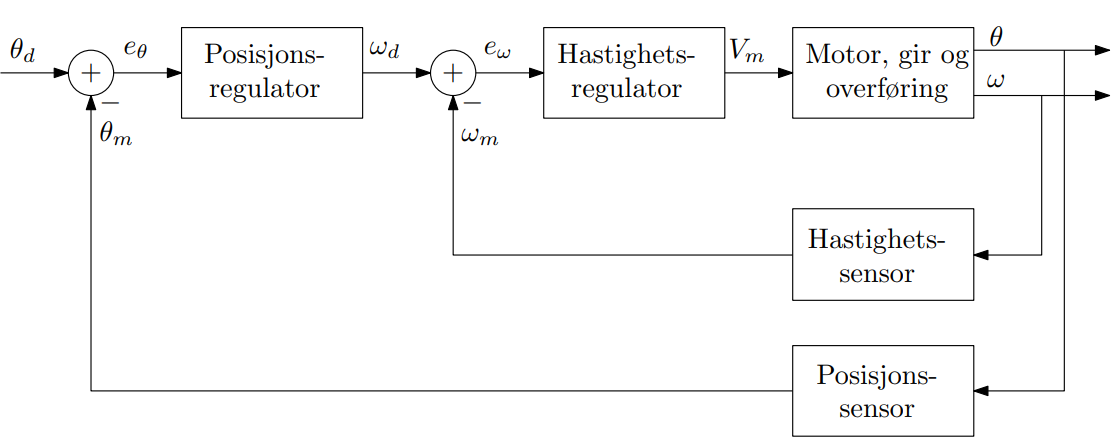
\includegraphics[width = 0.5\textwidth]{figurer/Blokkdiagram.png}
    \caption{Blokkdiagram........Må fikse størrelse}
    \label{fig:blokkdiagram}
\end{figure}





% Introduksjonen skal inneholde en oversikt over arbeidet dere har gjort, samt noen setninger som gir en videre kontekst for arbeidet (hva er nytten av å gjøre det dere har gjort i den store sammenhengen?). Dere kan også gjerne gi en kort beskrivelse av hvordan rapporten er organisert.

% Dere bør selvsagt legge mest fokus på å gjøre godt arbeid på labben, og å
% presentere det dere har gjort. Når det er sagt, er både innhold og
% presentasjon viktig. Husk at rapporten er deres eneste mulighet til å vise
% frem innsatsen dere har gjort, og hvordan dere legger det frem er derfor
% viktig. Hvis arbeidet dere har gjort på labben er fantastisk, men dere ikke
% klarer å formidle det i rapporten, så er det lite sannsynlig at dere får 
% uttelling for det. En figur som viser hvor bra regulatoren deres fungerer
% har liten verdi dersom den mangler en skikkelig beskrivelse av hva som blir
% vist. Husk også at gode diskusjoner av resultatene er viktig for å vise frem
% at dere forstår hva dere har gjort, og hvordan systemet fungerer.

% Layout er mindre viktig enn innhold, men det er fortsatt viktig. Dere kan
% tenke på rapportskriving som å skulle selge en leilighet; når du har 
% visning har du selvsagt vasket og ryddet for at den skal se så fin ut som
% mulig. Hvor ren leiligheten er avgjør selvsagt ikke verdien til leiligheten,
% men den påvirker hvilken subjektiv verdi kjøperne setter på leiligheten.
% På samme måte vil en rapport som ser pen og ryddig ut være enklere å lese, 
% og det er større sannsynlighet for at leseren får med seg det dere prøver å
% formidle.

% \subsection{Programvare}
% Dere står fritt til å velge programvare for rapportskriving.
% Dere kan for eksempel bruke Word eller andre tilsvarende programmer. 
% Ulempen med slike programmer er at det ofte er vanskelig (og av og til umulig)
% å få en god layout. Støtte for vektorgrafikk (forklares mer senere) er dårlig,
% og teksten ser sjelden like bra ut. På toppen av dette er det både vanskeligere
% å inkludere matematiske uttrykk, og resultater blir sjelden bra. Generelt vil 
% en rapport skrevet i Word ligne mer på et utkast enn en endelig rapport.

% Å bruke \LaTeX er sterkt anbefalt. Da er du nesten garantert at rapporten ser 
% bra ut, med mindre du gjør store endringer på konfigurasjonen. Det kan ta litt tid
% å komme i gang, men dere vil få utbytte av denne innsatsen både mot slutten av 
% rapportskrivingen, samt i senere fag og på masteroppgaven. \LaTeX har også 
% utmerket støtte for både matematiske uttrykk og vektorgrafikk.

%\section{Teori}

Tror denne delen kan være smud for å skrive ned et par ting her. Men det er viktig at vi koordinerer hva som står her :)

\begin{itemize}
    \item P-regulator
    \item PI-regulator
\end{itemize}
\input{hastighetsmåler}
\section{Hastighetsregulator}\label{sec:hastighetsreg}


\subsection{Teori}

Regulatorer brukes for å styre tilstander i en prosess. En regulator får inn et avvik mellom referansen og den målte tilstanden. Regulatorer bruker avviket til å beregne et pådrag til prosessen. P-regulator er en type regulator som lager et pådrag, $u$,  som er proporsjonalt med avviket, $e = \omega_d - \omega_m$. $K_p$ er proporsjonalitetsleddet i regulatoren, uttrykket for denne regulatoren er slik

\begin{equation}
    \label{eq:P_regulator}
    u(t) = K_p e(t).
\end{equation}

En slik regulator er effektiv så lenge det ikke er en kraft som forhindrer systemet å oppnå en spesifikk tilstand. Da vil ikke regulatoren regulere tilstanden helt til referanseverdien og det oppstår et stasjonæravvik. Friksjon og luftmotstand er krefter som vil motvirke at et system oppnår en hastighet større enn $0$. Et integratorledd vil motvirke slike krefter, ved å gi et pådrag tilsvarende disse kreftene. Da vil tilstanden nå referansetilstanden og det stasjonære avviket forsvinner. Uttrykk \eqref{eq:PI_regulator} beskriver en PI-regulator,

\begin{equation}
    \label{eq:PI_regulator}
    u(t) = K_p e(t) + \frac{K_p}{T_i} \int_{0}^{t} e(\tau) d\tau,
\end{equation}

der $u$ er pådraget, $K_p$ er proporsjonalitetskontanten, $e$ er avviket mellom referansen og tilstanden og $T_i$ er integratorkonstanten som representerer tidskonstanten til regulatoren.







\subsection{Metode}

\begin{figure}[b]
    \centering
    \begin{circuitikz} [scale=0.5, transform shape]
    \ctikzset{resistor = european}

    % --- OP1 ---
    \node[op amp](OP1) {$OP1$};
    
    \draw (OP1.-)
    to[R, l_=$R_1$] ++(-2, 0)
    to[short, o-, l=$\omega_m$] ++(0, 0);

    \draw (OP1.+)
    to[R=$R_1$] ++(-2, 0)
    to[short, o-, l=$\omega_d$] ++(0, 0);

    \draw (OP1.+)
    to[R=$R_2$, *-] ++(0, -2)
    node[ground] {};

    \draw (OP1.-)
    to[short, *-] ++(0, 1)
    coordinate(t1)
    to[R=$R_2$] (t1 -| OP1.out)
    -- (OP1.out);

    % --- OP2 ---

    \draw (OP1.out)
    to[short, *-, l=$e$] ++(0.5, 0)
    to[R=$R_3$] ++(2, 0)
    node[op amp, anchor=-](OP2) {$OP2$};

    \draw (OP2.-)
    to[short, *-] ++(0, 1)
    coordinate(t2)
    to[R=$R_4$] (t2 -| OP2.out)
    -- (OP2.out);

    \draw (OP2.+)
    node[ground] {};

    \draw (OP2.out)
    to[short, *-] ++(0, 0)
    to[R=$R_7$] ++(0, -2)
    coordinate(t7);

    % --- OP3 ---

    \draw (OP1.out)
    -- ++(0, -2)
    to[potentiometer, n=R5, l=$R_5$] ++(0, -2)
    coordinate(t3);

    \draw (R5.wiper)
    -- (R5.wiper |- t3)
    -- (t3);

    \draw (t3)
    to[short, *-] ++(0, -1)
    to[R=$R_6$] ++(2, 0)
    node[op amp, anchor=-](OP3) {$OP3$};

    \draw (OP3.+)
    node[ground] {};
    
    \draw (OP3.-)
    to[short, *-] ++(0, 1)
    coordinate(t4)
    to[C=$C_1$] (t4 -| OP3.out)
    coordinate(t5)
    -- (OP3.out);

    \draw (t4)
    to[short, *-] ++(0, 1.3)
    coordinate(t6)
    to[open jumper, l=$JP1$] (t6 -| t5)
    to[short, -*] (t5);

    \draw (OP3.out)
    to[short, *-] (OP3.out -| OP2.out)
    to[R, l_=$R_7$] ++(0, 2)
    coordinate (t8)
    to[short, *-*] (t7);

    % --- OP4 ---

    \draw (t8)
    -- ++(1.5, 0)
    node[op amp, anchor=-](OP4) {$OP4$};

    \draw (OP4.+)
    node[ground] {};

    \draw (t7)
    to[R=$R_8$] ++(2, 0)
    coordinate(t9)
    to[potentiometer, n=R9, l=$R_9$] (t9 -| OP4.out)
    coordinate(t10)
    -- (OP4.out);

    \draw (R9.wiper)
    -- (R9.wiper -| t10)
    to[short, -*] (t10);

    \draw (OP4.out)
    to[short, *-o, l=$V_m$] ++(1, 0);
    
\end{circuitikz}
    \caption{PI-regulator krets for hastighetsregulatoren. Figuren er hentet fra \cite{AnalogMotorlabbOppgaver}.}
    \label{fig:krets_hastighets_regulator}
\end{figure}

Hastighetsregulatoren ble implementert som en analog PI-regulator som vist i \autoref{fig:krets_hastighets_regulator}. $OP1$ er en differensialforsterker som finner avviket $e$, transferfunksjonen er gitt ved \eqref{eq:differensialforsterker}.
$OP2$ er en inverterende forsterker som inverterer avviket, uten forsterkning eller demping.
$OP3$ er en integrerende forsterker som integrerer $e$ og forsterker den med $\frac{1}{T_i}$. $JP1$ brukes for å nullstille integratoren og skru av I-leddet i integratoren. Da vil regulatoren oppføre seg som en P-regulator. Transferfunksjonen til $OP3$ er $-\frac{1}{(R_5 + R_6) C_1} \int e dt$. Dersom $JP1$ er kortsluttet er spenningen ut fra $OP3$ alltid {\SI{0}{\volt}}.
$OP4$ summerer spenningen fra $OP2$ og $OP3$ og forsterker resultatet med $K_p$. Transferfunksjonen for $OP4$ er $-\frac{R_8 + R_9}{R_7}(v_2 + v_3)$, der $v_2$ er spenningen ut av $OP2$ og $v_3$ er spenningen ut av $OP3$. Ut fra dette kommer et uttrykk for $K_p$ og $T_i$ som vist i \eqref{eq:K_p_og_T_i}.

\begin{equation}
    \label{eq:K_p_og_T_i}
    K_p = \frac{R_2}{R_1} \frac{R_8 + R_9}{R_7}, 
    T_i = (R_5 + R_6) C_1.
\end{equation}

Størrelsen på motstandene og kondensatoren er vist i likning \eqref{tab:Komponenter_i_hastighetsregulatoren}.

\begin{table}[h]
    \centering
    \caption{Motstander og kondensatorer i hastighetsregulatoren. Verdiene er hentet fra \cite{AnalogMotorlabbOppgaver}.}
    \begin{tabular}{lll}
        \toprule
        Størrelse & Verdi & Type \\
		\midrule
        $R_1$, $R_2$ & \SI{100}{\kilo\ohm} & Resistor\\
        $R_3$, $R_4$, $R_7$, $R_8$ & \SI{10}{\kilo\ohm} & Resistor \\
        $R_5$, $R_9$ & \SI{1}{\mega\ohm} & Potmeter \\
        $R_6$ & \SI{1}{\kilo\ohm} & Resistor \\
        $C_1$ & \SI{1}{\micro\farad} & Kondensator \\
        \bottomrule
    \end{tabular}
    \label{tab:Komponenter_i_hastighetsregulatoren}
\end{table}






\subsection{Resultater}

\label{obs:hastighet_regulator_breming_med_finger}
Det ble observert at stasjonæravviket og pådraget økte, dersom motoren ble bremset med en finger, da motoren ble regulert ved bruk av P-regulatoren. Ved bruk av PI-regulator økte pådraget til tilstanden nådde referanseverdien, selv med en finger som bremset motoren.

\begin{figure}[h]
    \centering
    % This file was created with tikzplotlib v0.10.1.
% Dette er eksempel data
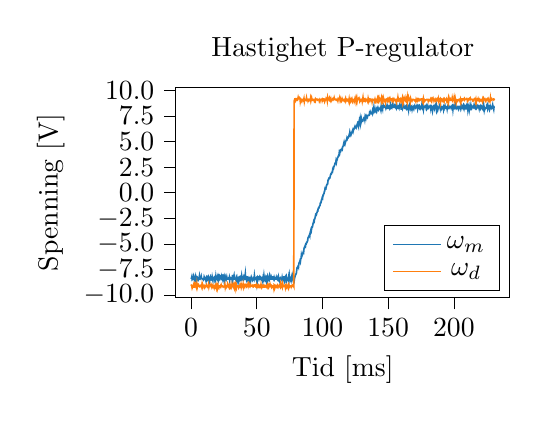
\begin{tikzpicture}

\definecolor{darkgray176}{RGB}{176,176,176}
\definecolor{darkorange25512714}{RGB}{255,127,14}
\definecolor{steelblue31119180}{RGB}{31,119,180}

\begin{axis}[
tick align=outside,
tick pos=left,
title={Hastighet P-regulator},
legend pos=south east,
height=\figH,
width=\figW,
x grid style={darkgray176},
xlabel={Tid [ms]},
xmin=-11.54538, xmax=242.45298,
xtick style={color=black},
xtick={-50,0,50,100,150,200,250},
xticklabels={
  \(\displaystyle {\ensuremath{-}50}\),
  \(\displaystyle {0}\),
  \(\displaystyle {50}\),
  \(\displaystyle {100}\),
  \(\displaystyle {150}\),
  \(\displaystyle {200}\),
  \(\displaystyle {250}\)
},
y grid style={darkgray176},
ylabel={Spenning [V]},
ymin=-10.231936, ymax=10.231936,
ytick style={color=black},
ytick={-12.5,-10,-7.5,-5,-2.5,0,2.5,5,7.5,10,12.5},
yticklabels={
  \(\displaystyle {\ensuremath{-}12.5}\),
  \(\displaystyle {\ensuremath{-}10.0}\),
  \(\displaystyle {\ensuremath{-}7.5}\),
  \(\displaystyle {\ensuremath{-}5.0}\),
  \(\displaystyle {\ensuremath{-}2.5}\),
  \(\displaystyle {0.0}\),
  \(\displaystyle {2.5}\),
  \(\displaystyle {5.0}\),
  \(\displaystyle {7.5}\),
  \(\displaystyle {10.0}\),
  \(\displaystyle {12.5}\)
}
]
\legend{$\omega_m$, $\omega_d$}
\addplot [semithick, steelblue31119180]
table {%
0 -8.42285
0.2772000000002 -8.37402
0.554400000000399 -8.22754
0.83159999999971 -8.47168
1.10879999999991 -8.42285
1.38600000000011 -8.42285
1.66320000000031 -8.37402
1.94039999999962 -8.12988
2.21759999999982 -8.22754
2.49480000000002 -8.47168
2.77200000000022 -8.37402
3.04919999999953 -8.47168
3.32639999999973 -8.22754
3.60359999999993 -8.42285
3.88080000000013 -8.3252
4.15800000000033 -8.61816
4.43519999999964 -8.3252
4.71239999999984 -8.27637
4.98960000000004 -8.37402
5.26680000000024 -8.47168
5.54399999999955 -8.52051
5.82119999999975 -8.42285
6.09839999999995 -8.3252
6.37560000000015 -8.12988
6.65280000000035 -8.37402
6.92999999999966 -8.42285
7.20719999999986 -8.37402
7.48440000000006 -8.3252
7.76160000000026 -8.17871
8.03879999999957 -8.37402
8.31599999999977 -8.37402
8.59319999999997 -8.42285
8.87040000000017 -8.42285
9.14760000000037 -8.42285
9.42479999999968 -8.52051
9.70199999999988 -8.47168
9.97920000000008 -8.22754
10.2564000000003 -8.3252
10.5335999999996 -8.37402
10.8107999999998 -8.42285
11.088 -8.47168
11.3652000000002 -8.61816
11.6424000000004 -8.22754
11.9195999999997 -8.17871
12.1967999999999 -8.27637
12.4740000000001 -8.42285
12.7512000000003 -8.3252
13.0283999999996 -8.42285
13.3055999999998 -8.27637
13.5828 -8.42285
13.8600000000002 -8.37402
14.1371999999995 -8.61816
14.4143999999997 -8.3252
14.6915999999999 -8.22754
14.9688000000001 -8.42285
15.2460000000003 -8.47168
15.5231999999996 -8.42285
15.8003999999998 -8.47168
16.0776 -8.22754
16.3548000000002 -8.42285
16.6319999999995 -8.56934
16.9091999999997 -8.3252
17.1863999999999 -8.37402
17.4636000000001 -8.3252
17.7408000000003 -8.27637
18.0179999999996 -8.47168
18.2951999999998 -8.3252
18.5724 -8.47168
18.8496000000002 -8.17871
19.1267999999996 -8.42285
19.4039999999998 -8.37402
19.6812 -8.42285
19.9584000000002 -8.22754
20.2356000000004 -8.12988
20.5127999999997 -8.42285
20.7899999999999 -8.61816
21.0672000000001 -8.52051
21.3444000000003 -8.47168
21.6215999999996 -8.08105
21.8987999999998 -8.12988
22.176 -8.3252
22.4532000000002 -8.22754
22.7304000000004 -8.3252
23.0075999999997 -8.37402
23.2847999999999 -8.17871
23.5620000000001 -8.3252
23.8392000000003 -8.22754
24.1163999999996 -8.42285
24.3935999999998 -8.27637
24.6708 -8.17871
24.9480000000002 -8.3252
25.2252000000004 -8.61816
25.5023999999997 -8.27637
25.7795999999999 -8.42285
26.0568000000001 -8.27637
26.3340000000003 -8.47168
26.6111999999996 -8.52051
26.8883999999998 -8.37402
27.1656 -8.22754
27.4428000000002 -8.42285
27.7199999999995 -8.42285
27.9971999999997 -8.42285
28.2743999999999 -8.37402
28.5516000000001 -8.42285
28.8288000000003 -8.42285
29.1059999999996 -8.27637
29.3831999999998 -8.52051
29.6604 -8.27637
29.9376000000002 -8.3252
30.2147999999995 -8.42285
30.4919999999997 -8.42285
30.7691999999999 -8.42285
31.0464000000001 -8.3252
31.3236000000003 -8.56934
31.6007999999997 -8.03223
31.8779999999999 -8.42285
32.1552000000001 -8.22754
32.4324000000002 -8.22754
32.7095999999996 -8.08105
32.9867999999998 -8.42285
33.264 -8.42285
33.5412000000002 -8.42285
33.8184000000004 -8.47168
34.0955999999997 -8.52051
34.3727999999999 -8.3252
34.6500000000001 -8.47168
34.9272000000003 -8.3252
35.2043999999996 -8.56934
35.4815999999998 -8.37402
35.7588 -8.37402
36.0360000000002 -8.3252
36.3132000000004 -8.61816
36.5903999999997 -8.3252
36.8675999999999 -8.27637
37.1448000000001 -8.22754
37.4220000000003 -8.42285
37.6991999999996 -8.56934
37.9763999999998 -8.56934
38.2536 -8.42285
38.5308000000002 -8.12988
38.8080000000004 -8.37402
39.0851999999997 -8.42285
39.3623999999999 -8.27637
39.6396000000001 -8.3252
39.9168000000003 -8.22754
40.1939999999996 -8.47168
40.4711999999998 -8.42285
40.7484 -8.42285
41.0256000000002 -8.22754
41.3027999999995 -7.93457
41.5799999999997 -8.37402
41.8571999999999 -8.42285
42.1344000000001 -8.52051
42.4116000000003 -8.22754
42.6887999999996 -8.22754
42.9659999999998 -8.42285
43.2432 -8.52051
43.5204000000002 -8.37402
43.7975999999995 -8.37402
44.0747999999997 -8.27637
44.3519999999999 -8.3252
44.6292000000001 -8.61816
44.9064000000003 -8.52051
45.1835999999997 -8.66699
45.4607999999999 -8.3252
45.7380000000001 -8.22754
46.0152000000003 -8.37402
46.2923999999996 -8.3252
46.5695999999998 -8.42285
46.8468 -8.56934
47.1240000000002 -8.52051
47.4012000000004 -8.42285
47.6783999999997 -8.3252
47.9555999999999 -8.42285
48.2328000000001 -8.08105
48.5100000000003 -8.3252
48.7871999999996 -8.37402
49.0643999999998 -8.42285
49.3416 -8.37402
49.6188000000002 -8.3252
49.8960000000004 -8.42285
50.1731999999997 -8.81348
50.4503999999999 -8.52051
50.7276000000001 -8.22754
51.0048000000003 -8.27637
51.2819999999996 -8.22754
51.5591999999998 -8.22754
51.8364 -8.42285
52.1136000000002 -8.3252
52.3907999999995 -8.17871
52.6679999999997 -8.22754
52.9451999999999 -8.42285
53.2224000000001 -8.47168
53.4996000000003 -8.27637
53.7767999999996 -8.27637
54.0539999999998 -8.27637
54.3312 -8.37402
54.6084000000002 -8.61816
54.8855999999995 -8.27637
55.1627999999997 -8.37402
55.4399999999999 -8.08105
55.7172000000001 -8.37402
55.9944000000003 -8.3252
56.2715999999996 -8.47168
56.5487999999998 -8.3252
56.826 -8.22754
57.1032000000002 -8.37402
57.3803999999996 -8.61816
57.6575999999998 -8.37402
57.9348 -8.47168
58.2120000000002 -8.27637
58.4892000000004 -8.52051
58.7663999999997 -8.37402
59.0435999999999 -8.42285
59.3208000000001 -8.27637
59.5980000000003 -8.12988
59.8751999999996 -8.42285
60.1523999999998 -8.3252
60.4296 -8.42285
60.7068000000002 -8.42285
60.9840000000004 -8.17871
61.2611999999997 -8.27637
61.5383999999999 -8.42285
61.8156000000001 -8.42285
62.0928000000003 -8.22754
62.3699999999996 -8.22754
62.6471999999998 -8.3252
62.9244 -8.42285
63.2016000000002 -8.27637
63.4788000000004 -8.42285
63.7559999999997 -8.3252
64.0331999999999 -8.37402
64.3104000000001 -8.42285
64.5876000000003 -8.42285
64.8647999999996 -8.27637
65.1419999999998 -8.42285
65.4192 -8.42285
65.6964000000002 -8.47168
65.9735999999995 -8.3252
66.2507999999997 -8.42285
66.5279999999999 -8.22754
66.8052000000001 -8.42285
67.0824000000003 -8.42285
67.3595999999996 -8.56934
67.6367999999998 -8.37402
67.914 -8.3252
68.1912000000002 -8.42285
68.4683999999995 -8.42285
68.7455999999997 -8.37402
69.0227999999999 -8.47168
69.3000000000001 -8.27637
69.5772000000003 -8.47168
69.8543999999997 -8.42285
70.1315999999998 -8.37402
70.4088 -8.47168
70.6860000000002 -8.22754
70.9631999999996 -8.22754
71.2403999999998 -8.52051
71.5176 -8.3252
71.7948000000002 -8.17871
72.0720000000004 -8.12988
72.3491999999997 -8.42285
72.6263999999999 -8.27637
72.9036000000001 -8.52051
73.1808000000003 -8.37402
73.4579999999996 -8.42285
73.7351999999998 -8.37402
74.0124 -8.47168
74.2896000000002 -8.22754
74.5668000000004 -8.47168
74.8439999999997 -8.12988
75.1211999999999 -8.42285
75.3984000000001 -8.42285
75.6756000000003 -8.52051
75.9527999999996 -8.37402
76.2299999999998 -8.37402
76.5072 -8.22754
76.7844000000002 -8.56934
77.0616000000004 -8.47168
77.3387999999997 -8.47168
77.6159999999999 -8.08105
77.8932000000001 -8.22754
78.1704000000003 -8.52051
78.4475999999996 -8.61816
78.7247999999998 -8.37402
79.002 -8.22754
79.2792000000002 -8.08105
79.5563999999995 -8.03223
79.8335999999997 -7.93457
80.1107999999999 -7.88574
80.3880000000001 -7.59277
80.6652000000003 -7.34863
80.9423999999996 -7.34863
81.2195999999998 -7.20215
81.4968 -7.15332
81.7740000000002 -7.25098
82.0511999999995 -6.90918
82.3283999999997 -6.81152
82.6056 -6.81152
82.8828000000001 -6.66504
83.1600000000003 -6.7627
83.4371999999996 -6.46973
83.7143999999999 -6.4209
83.9916000000001 -6.0791
84.2688000000003 -6.22559
84.5459999999996 -6.12793
84.8231999999998 -6.03027
85.1004 -5.88379
85.3776000000002 -5.78613
85.6548000000004 -5.83496
85.9319999999997 -5.49316
86.2091999999999 -5.34668
86.4864000000001 -5.29785
86.7636000000003 -5.2002
87.0407999999996 -5.24902
87.3179999999998 -5.00488
87.5952 -5.00488
87.8724000000002 -4.8584
88.1496000000004 -4.8584
88.4267999999997 -4.76074
88.7039999999999 -4.71191
88.9812000000001 -4.41895
89.2584000000003 -4.37012
89.5355999999996 -4.27246
89.8127999999998 -4.22363
90.09 -4.12598
90.3672000000002 -4.22363
90.6443999999995 -3.88184
90.9215999999997 -3.78418
91.1987999999999 -3.6377
91.4760000000001 -3.73535
91.7532000000003 -3.49121
92.0303999999996 -3.34473
92.3075999999998 -3.34473
92.5848 -3.19824
92.8620000000002 -3.00293
93.1391999999995 -2.90527
93.4163999999997 -2.75879
93.6935999999999 -2.80762
93.9708000000001 -2.56348
94.2480000000003 -2.51465
94.5251999999996 -2.36816
94.8023999999998 -2.17285
95.0796 -2.22168
95.3568000000002 -2.17285
95.6339999999996 -1.97754
95.9111999999998 -1.92871
96.1883999999999 -1.78223
96.4656000000002 -1.78223
96.7428000000004 -1.53809
97.0199999999997 -1.48926
97.2971999999999 -1.48926
97.5744000000001 -1.34277
97.8516000000003 -1.29395
98.1287999999996 -1.24512
98.4059999999998 -1.00098
98.6832 -0.952148
98.9604000000002 -0.952148
99.2376000000004 -0.708008
99.5147999999997 -0.65918
99.7919999999999 -0.512695
100.0692 -0.561523
100.3464 -0.268555
100.6236 -0.268555
100.9008 -0.12207
101.178 -0.0732422
101.4552 0.12207
101.7324 0.170898
102.0096 0.415039
102.2868 0.366211
102.564 0.366211
102.8412 0.561523
103.1184 0.708008
103.3956 0.805664
103.6728 0.805664
103.95 0.854492
104.2272 1.19629
104.5044 1.29395
104.7816 1.29395
105.0588 1.44043
105.336 1.44043
105.6132 1.44043
105.8904 1.58691
106.1676 1.7334
106.4448 1.83105
106.722 1.83105
106.9992 1.97754
107.2764 1.97754
107.5536 1.97754
107.8308 2.31934
108.108 2.41699
108.3852 2.36816
108.6624 2.51465
108.9396 2.6123
109.2168 2.66113
109.494 2.85645
109.7712 2.85645
110.0484 2.85645
110.3256 3.10059
110.6028 2.9541
110.88 3.14941
111.1572 3.19824
111.4344 3.39355
111.7116 3.44238
111.9888 3.54004
112.266 3.6377
112.5432 3.6377
112.8204 3.93066
113.0976 3.83301
113.3748 4.02832
113.652 4.12598
113.9292 4.07715
114.2064 4.1748
114.4836 4.22363
114.7608 4.27246
115.038 4.22363
115.3152 4.46777
115.5924 4.5166
115.8696 4.56543
116.1468 4.76074
116.424 4.90723
116.7012 4.71191
116.9784 4.66309
117.2556 4.80957
117.5328 4.95605
117.81 5.05371
118.0872 5.10254
118.3644 5.2002
118.6416 5.34668
118.9188 5.24902
119.196 5.34668
119.4732 5.34668
119.7504 5.44434
120.0276 5.49316
120.3048 5.63965
120.582 5.59082
120.8592 5.88379
121.1364 5.7373
121.4136 5.7373
121.6908 5.63965
121.968 5.7373
122.2452 5.88379
122.5224 5.93262
122.7996 6.03027
123.0768 6.12793
123.354 5.98145
123.6312 6.12793
123.9084 6.17676
124.1856 6.27441
124.4628 6.37207
124.74 6.46973
125.0172 6.37207
125.2944 6.37207
125.5716 6.32324
125.8488 6.46973
126.126 6.51855
126.4032 6.66504
126.6804 6.7627
126.9576 6.66504
127.2348 6.51855
127.512 6.81152
127.7892 6.7627
128.0664 7.00684
128.3436 6.86035
128.6208 7.10449
128.898 6.61621
129.1752 6.7627
129.4524 6.86035
129.7296 7.20215
130.0068 7.05566
130.284 6.95801
130.5612 6.95801
130.8384 7.10449
131.1156 7.10449
131.3928 7.15332
131.67 7.34863
131.9472 7.34863
132.2244 7.15332
132.5016 7.44629
132.7788 7.34863
133.056 7.25098
133.3332 7.44629
133.6104 7.34863
133.8876 7.39746
134.1648 7.34863
134.442 7.54395
134.7192 7.54395
134.9964 7.54395
135.2736 7.54395
135.5508 7.54395
135.828 7.78809
136.1052 7.73926
136.3824 7.88574
136.6596 7.78809
136.9368 7.78809
137.214 7.73926
137.4912 7.78809
137.7684 7.83691
138.0456 7.9834
138.3228 7.73926
138.6 7.83691
138.8772 8.03223
139.1544 8.3252
139.4316 8.08105
139.7088 7.9834
139.986 8.12988
140.2632 8.12988
140.5404 8.03223
140.8176 8.22754
141.0948 8.12988
141.372 7.9834
141.6492 8.12988
141.9264 8.22754
142.2036 8.3252
142.4808 8.22754
142.758 8.08105
143.0352 8.12988
143.3124 8.12988
143.5896 8.22754
143.8668 8.27637
144.144 8.22754
144.4212 8.08105
144.6984 8.42285
144.9756 8.22754
145.2528 8.37402
145.53 8.3252
145.8072 8.17871
146.0844 8.52051
146.3616 8.56934
146.6388 8.42285
146.916 8.42285
147.1932 8.3252
147.4704 8.3252
147.7476 8.42285
148.0248 8.37402
148.302 8.22754
148.5792 8.3252
148.8564 8.37402
149.1336 8.52051
149.4108 8.3252
149.688 8.22754
149.9652 8.22754
150.2424 8.42285
150.5196 8.37402
150.7968 8.42285
151.074 8.3252
151.3512 8.17871
151.6284 8.22754
151.9056 8.52051
152.1828 8.3252
152.46 8.3252
152.7372 8.27637
153.0144 8.42285
153.2916 8.56934
153.5688 8.37402
153.846 8.3252
154.1232 8.3252
154.4004 8.3252
154.6776 8.56934
154.9548 8.52051
155.232 8.37402
155.5092 8.3252
155.7864 8.27637
156.0636 8.52051
156.3408 8.3252
156.618 8.47168
156.8952 8.22754
157.1724 8.22754
157.4496 8.37402
157.7268 8.42285
158.004 8.37402
158.2812 8.27637
158.5584 8.52051
158.8356 8.61816
159.1128 8.42285
159.39 8.42285
159.6672 8.47168
159.9444 8.08105
160.2216 8.42285
160.4988 8.56934
160.776 8.47168
161.0532 8.22754
161.3304 8.3252
161.6076 8.37402
161.8848 8.52051
162.162 8.37402
162.4392 8.3252
162.7164 8.22754
162.9936 8.22754
163.2708 8.42285
163.548 8.47168
163.8252 8.17871
164.1024 8.12988
164.3796 8.17871
164.6568 8.42285
164.934 8.37402
165.2112 8.27637
165.4884 8.08105
165.7656 8.52051
166.0428 8.52051
166.32 8.61816
166.5972 8.37402
166.8744 8.22754
167.1516 8.37402
167.4288 8.27637
167.706 8.42285
167.9832 8.37402
168.2604 8.12988
168.5376 8.27637
168.8148 8.22754
169.092 8.42285
169.3692 8.37402
169.6464 8.22754
169.9236 8.37402
170.2008 8.47168
170.478 8.3252
170.7552 8.27637
171.0324 8.37402
171.3096 8.42285
171.5868 8.47168
171.864 8.52051
172.1412 8.37402
172.4184 8.17871
172.6956 8.37402
172.9728 8.47168
173.25 8.42285
173.5272 8.47168
173.8044 8.22754
174.0816 8.17871
174.3588 8.42285
174.636 8.37402
174.9132 8.27637
175.1904 8.3252
175.4676 8.27637
175.7448 8.61816
176.022 8.42285
176.2992 8.56934
176.5764 8.37402
176.8536 8.12988
177.1308 8.37402
177.408 8.3252
177.6852 8.37402
177.9624 8.42285
178.2396 8.52051
178.5168 8.52051
178.794 8.3252
179.0712 8.42285
179.3484 8.12988
179.6256 8.17871
179.9028 8.3252
180.18 8.47168
180.4572 8.37402
180.7344 8.27637
181.0116 8.3252
181.2888 8.42285
181.566 8.42285
181.8432 8.47168
182.1204 8.37402
182.3976 8.17871
182.6748 8.42285
182.952 8.47168
183.2292 8.42285
183.5064 8.27637
183.7836 8.03223
184.0608 8.27637
184.338 8.27637
184.6152 8.42285
184.8924 8.37402
185.1696 8.22754
185.4468 8.42285
185.724 8.56934
186.0012 8.61816
186.2784 8.47168
186.5556 8.22754
186.8328 8.47168
187.11 8.17871
187.3872 8.42285
187.6644 8.37402
187.9416 8.17871
188.2188 8.3252
188.496 8.3252
188.7732 8.3252
189.0504 8.47168
189.3276 8.37402
189.6048 8.22754
189.882 8.52051
190.1592 8.37402
190.4364 8.37402
190.7136 8.22754
190.9908 8.3252
191.268 8.3252
191.5452 8.37402
191.8224 8.3252
192.0996 8.12988
192.3768 8.37402
192.654 8.27637
192.9312 8.47168
193.2084 8.52051
193.4856 8.22754
193.7628 8.22754
194.04 8.27637
194.3172 8.37402
194.5944 8.37402
194.8716 8.17871
195.1488 8.42285
195.426 8.52051
195.7032 8.56934
195.9804 8.3252
196.2576 8.37402
196.5348 8.27637
196.812 8.3252
197.0892 8.42285
197.3664 8.42285
197.6436 8.37402
197.9208 8.27637
198.198 8.42285
198.4752 8.47168
198.7524 8.52051
199.0296 8.47168
199.3068 8.12988
199.584 8.42285
199.8612 8.3252
200.1384 8.42285
200.4156 8.27637
200.6928 8.22754
200.97 8.37402
201.2472 8.56934
201.5244 8.37402
201.8016 8.27637
202.0788 8.22754
202.356 8.37402
202.6332 8.42285
202.9104 8.42285
203.1876 8.37402
203.4648 8.22754
203.742 8.37402
204.0192 8.42285
204.2964 8.42285
204.5736 8.37402
204.8508 8.22754
205.128 8.42285
205.4052 8.42285
205.6824 8.56934
205.9596 8.52051
206.2368 8.27637
206.514 8.37402
206.7912 8.37402
207.0684 8.47168
207.3456 8.27637
207.6228 8.17871
207.9 8.47168
208.1772 8.37402
208.4544 8.37402
208.7316 8.42285
209.0088 8.17871
209.286 8.17871
209.5632 8.37402
209.8404 8.52051
210.1176 8.42285
210.3948 8.52051
210.672 8.12988
210.9492 8.37402
211.2264 8.27637
211.5036 8.42285
211.7808 8.12988
212.058 8.37402
212.3352 8.42285
212.6124 8.3252
212.8896 8.52051
213.1668 8.22754
213.444 8.17871
213.7212 8.27637
213.9984 8.42285
214.2756 8.37402
214.5528 8.37402
214.83 8.3252
215.1072 8.42285
215.3844 8.56934
215.6616 8.42285
215.9388 8.27637
216.216 8.22754
216.4932 8.37402
216.7704 8.56934
217.0476 8.37402
217.3248 8.22754
217.602 8.27637
217.8792 8.47168
218.1564 8.52051
218.4336 8.42285
218.7108 8.3252
218.988 8.3252
219.2652 8.17871
219.5424 8.37402
219.8196 8.3252
220.0968 8.42285
220.374 8.27637
220.6512 8.42285
220.9284 8.47168
221.2056 8.42285
221.4828 8.3252
221.76 8.17871
222.0372 8.12988
222.3144 8.42285
222.5916 8.66699
222.8688 8.37402
223.146 8.08105
223.4232 8.27637
223.7004 8.17871
223.9776 8.27637
224.2548 8.27637
224.532 8.22754
224.8092 8.22754
225.0864 8.56934
225.3636 8.61816
225.6408 8.66699
225.918 8.17871
226.1952 8.27637
226.4724 8.42285
226.7496 8.47168
227.0268 8.42285
227.304 8.12988
227.5812 8.22754
227.8584 8.42285
228.1356 8.3252
228.4128 8.27637
228.69 8.22754
228.9672 8.3252
229.2444 8.42285
229.5216 8.56934
229.7988 8.37402
230.076 8.27637
230.3532 8.12988
230.6304 8.42285
230.9076 8.42285
};
\addplot [semithick, darkorange25512714]
table {%
0 -8.95996
0.2772000000002 -9.05762
0.554400000000399 -9.10645
0.83159999999971 -9.30176
1.10879999999991 -9.2041
1.38600000000011 -9.15527
1.66320000000031 -9.05762
1.94039999999962 -8.95996
2.21759999999982 -9.2041
2.49480000000002 -9.2041
2.77200000000022 -8.95996
3.04919999999953 -9.05762
3.32639999999973 -8.95996
3.60359999999993 -9.15527
3.88080000000013 -9.2041
4.15800000000033 -9.30176
4.43519999999964 -8.95996
4.71239999999984 -9.25293
4.98960000000004 -9.10645
5.26680000000024 -9.10645
5.54399999999955 -9.00879
5.82119999999975 -9.10645
6.09839999999995 -9.10645
6.37560000000015 -9.15527
6.65280000000035 -9.10645
6.92999999999966 -9.05762
7.20719999999986 -9.10645
7.48440000000006 -9.15527
7.76160000000026 -9.10645
8.03879999999957 -9.2041
8.31599999999977 -8.95996
8.59319999999997 -9.15527
8.87040000000017 -8.95996
9.14760000000037 -9.05762
9.42479999999968 -9.10645
9.70199999999988 -9.15527
9.97920000000008 -9.25293
10.2564000000003 -9.15527
10.5335999999996 -9.25293
10.8107999999998 -9.2041
11.088 -9.10645
11.3652000000002 -9.10645
11.6424000000004 -9.00879
11.9195999999997 -9.10645
12.1967999999999 -9.10645
12.4740000000001 -9.2041
12.7512000000003 -9.15527
13.0283999999996 -9.10645
13.3055999999998 -8.95996
13.5828 -9.2041
13.8600000000002 -9.05762
14.1371999999995 -9.00879
14.4143999999997 -9.00879
14.6915999999999 -9.05762
14.9688000000001 -9.10645
15.2460000000003 -8.95996
15.5231999999996 -9.05762
15.8003999999998 -9.2041
16.0776 -9.10645
16.3548000000002 -9.15527
16.6319999999995 -9.05762
16.9091999999997 -9.2041
17.1863999999999 -9.10645
17.4636000000001 -9.10645
17.7408000000003 -9.10645
18.0179999999996 -9.25293
18.2951999999998 -9.10645
18.5724 -9.25293
18.8496000000002 -9.2041
19.1267999999996 -9.05762
19.4039999999998 -9.25293
19.6812 -9.00879
19.9584000000002 -8.95996
20.2356000000004 -9.25293
20.5127999999997 -9.05762
20.7899999999999 -9.25293
21.0672000000001 -9.30176
21.3444000000003 -9.10645
21.6215999999996 -9.10645
21.8987999999998 -9.15527
22.176 -9.2041
22.4532000000002 -9.10645
22.7304000000004 -9.15527
23.0075999999997 -9.00879
23.2847999999999 -9.10645
23.5620000000001 -9.10645
23.8392000000003 -9.10645
24.1163999999996 -9.15527
24.3935999999998 -9.2041
24.6708 -9.15527
24.9480000000002 -9.15527
25.2252000000004 -9.15527
25.5023999999997 -9.10645
25.7795999999999 -8.95996
26.0568000000001 -9.25293
26.3340000000003 -9.10645
26.6111999999996 -9.10645
26.8883999999998 -9.25293
27.1656 -9.2041
27.4428000000002 -9.15527
27.7199999999995 -8.95996
27.9971999999997 -9.10645
28.2743999999999 -9.15527
28.5516000000001 -9.10645
28.8288000000003 -9.2041
29.1059999999996 -9.00879
29.3831999999998 -9.10645
29.6604 -9.05762
29.9376000000002 -9.30176
30.2147999999995 -9.25293
30.4919999999997 -9.00879
30.7691999999999 -9.2041
31.0464000000001 -9.10645
31.3236000000003 -9.10645
31.6007999999997 -9.10645
31.8779999999999 -8.95996
32.1552000000001 -9.10645
32.4324000000002 -9.2041
32.7095999999996 -9.05762
32.9867999999998 -9.25293
33.264 -9.10645
33.5412000000002 -9.30176
33.8184000000004 -8.95996
34.0955999999997 -9.10645
34.3727999999999 -9.00879
34.6500000000001 -9.25293
34.9272000000003 -9.10645
35.2043999999996 -9.15527
35.4815999999998 -9.15527
35.7588 -9.10645
36.0360000000002 -9.10645
36.3132000000004 -9.25293
36.5903999999997 -9.15527
36.8675999999999 -9.15527
37.1448000000001 -9.05762
37.4220000000003 -9.15527
37.6991999999996 -9.10645
37.9763999999998 -8.95996
38.2536 -9.2041
38.5308000000002 -9.05762
38.8080000000004 -9.15527
39.0851999999997 -9.15527
39.3623999999999 -9.2041
39.6396000000001 -8.95996
39.9168000000003 -9.2041
40.1939999999996 -9.05762
40.4711999999998 -9.05762
40.7484 -9.00879
41.0256000000002 -9.15527
41.3027999999995 -9.05762
41.5799999999997 -9.05762
41.8571999999999 -8.95996
42.1344000000001 -8.95996
42.4116000000003 -9.15527
42.6887999999996 -9.10645
42.9659999999998 -9.10645
43.2432 -8.95996
43.5204000000002 -9.10645
43.7975999999995 -8.95996
44.0747999999997 -9.10645
44.3519999999999 -9.10645
44.6292000000001 -9.15527
44.9064000000003 -8.95996
45.1835999999997 -9.05762
45.4607999999999 -9.10645
45.7380000000001 -9.05762
46.0152000000003 -9.10645
46.2923999999996 -9.10645
46.5695999999998 -9.10645
46.8468 -9.05762
47.1240000000002 -9.15527
47.4012000000004 -9.10645
47.6783999999997 -9.15527
47.9555999999999 -9.10645
48.2328000000001 -9.00879
48.5100000000003 -9.00879
48.7871999999996 -9.10645
49.0643999999998 -9.15527
49.3416 -9.10645
49.6188000000002 -9.00879
49.8960000000004 -9.15527
50.1731999999997 -9.25293
50.4503999999999 -9.2041
50.7276000000001 -9.10645
51.0048000000003 -9.15527
51.2819999999996 -9.00879
51.5591999999998 -9.05762
51.8364 -9.2041
52.1136000000002 -9.25293
52.3907999999995 -9.25293
52.6679999999997 -9.10645
52.9451999999999 -9.15527
53.2224000000001 -8.95996
53.4996000000003 -9.15527
53.7767999999996 -9.25293
54.0539999999998 -9.15527
54.3312 -9.10645
54.6084000000002 -9.05762
54.8855999999995 -9.15527
55.1627999999997 -9.10645
55.4399999999999 -9.2041
55.7172000000001 -9.2041
55.9944000000003 -9.10645
56.2715999999996 -9.15527
56.5487999999998 -9.10645
56.826 -9.15527
57.1032000000002 -9.10645
57.3803999999996 -9.2041
57.6575999999998 -9.15527
57.9348 -9.2041
58.2120000000002 -9.05762
58.4892000000004 -9.2041
58.7663999999997 -9.10645
59.0435999999999 -9.2041
59.3208000000001 -9.05762
59.5980000000003 -9.15527
59.8751999999996 -9.10645
60.1523999999998 -8.95996
60.4296 -9.10645
60.7068000000002 -9.15527
60.9840000000004 -9.10645
61.2611999999997 -9.2041
61.5383999999999 -9.10645
61.8156000000001 -9.15527
62.0928000000003 -9.2041
62.3699999999996 -9.10645
62.6471999999998 -9.10645
62.9244 -9.30176
63.2016000000002 -9.00879
63.4788000000004 -9.05762
63.7559999999997 -9.30176
64.0331999999999 -9.2041
64.3104000000001 -9.10645
64.5876000000003 -9.15527
64.8647999999996 -9.15527
65.1419999999998 -9.2041
65.4192 -9.05762
65.6964000000002 -9.00879
65.9735999999995 -9.10645
66.2507999999997 -9.2041
66.5279999999999 -9.10645
66.8052000000001 -9.10645
67.0824000000003 -9.05762
67.3595999999996 -9.15527
67.6367999999998 -9.2041
67.914 -9.25293
68.1912000000002 -8.95996
68.4683999999995 -9.15527
68.7455999999997 -9.2041
69.0227999999999 -9.15527
69.3000000000001 -8.95996
69.5772000000003 -9.15527
69.8543999999997 -8.95996
70.1315999999998 -9.10645
70.4088 -9.15527
70.6860000000002 -9.15527
70.9631999999996 -9.10645
71.2403999999998 -9.10645
71.5176 -9.05762
71.7948000000002 -9.25293
72.0720000000004 -9.05762
72.3491999999997 -9.10645
72.6263999999999 -9.2041
72.9036000000001 -9.05762
73.1808000000003 -9.15527
73.4579999999996 -9.15527
73.7351999999998 -9.25293
74.0124 -9.10645
74.2896000000002 -9.25293
74.5668000000004 -9.05762
74.8439999999997 -9.2041
75.1211999999999 -9.15527
75.3984000000001 -9.10645
75.6756000000003 -9.10645
75.9527999999996 -9.10645
76.2299999999998 -9.2041
76.5072 -9.10645
76.7844000000002 -9.05762
77.0616000000004 -9.10645
77.3387999999997 -9.05762
77.6159999999999 -9.10645
77.8932000000001 -9.00879
78.1704000000003 -9.10645
78.4475999999996 8.91113
78.7247999999998 9.05762
79.002 9.15527
79.2792000000002 9.15527
79.5563999999995 9.00879
79.8335999999997 9.10645
80.1107999999999 9.05762
80.3880000000001 9.10645
80.6652000000003 9.00879
80.9423999999996 9.00879
81.2195999999998 9.15527
81.4968 9.30176
81.7740000000002 9.15527
82.0511999999995 9.15527
82.3283999999997 9.15527
82.6056 9.25293
82.8828000000001 9.2041
83.1600000000003 8.8623
83.4371999999996 9.00879
83.7143999999999 9.10645
83.9916000000001 9.05762
84.2688000000003 8.95996
84.5459999999996 9.10645
84.8231999999998 9.10645
85.1004 9.10645
85.3776000000002 9.00879
85.6548000000004 9.05762
85.9319999999997 9.2041
86.2091999999999 8.91113
86.4864000000001 9.10645
86.7636000000003 9.10645
87.0407999999996 9.00879
87.3179999999998 9.00879
87.5952 9.05762
87.8724000000002 9.25293
88.1496000000004 9.05762
88.4267999999997 9.10645
88.7039999999999 9.10645
88.9812000000001 8.95996
89.2584000000003 9.05762
89.5355999999996 9.00879
89.8127999999998 9.10645
90.09 9.10645
90.3672000000002 9.05762
90.6443999999995 9.00879
90.9215999999997 9.2041
91.1987999999999 8.95996
91.4760000000001 9.10645
91.7532000000003 9.25293
92.0303999999996 9.10645
92.3075999999998 9.05762
92.5848 9.10645
92.8620000000002 9.10645
93.1391999999995 9.05762
93.4163999999997 9.10645
93.6935999999999 9.10645
93.9708000000001 8.91113
94.2480000000003 8.95996
94.5251999999996 8.91113
94.8023999999998 9.15527
95.0796 9.10645
95.3568000000002 9.05762
95.6339999999996 9.05762
95.9111999999998 9.10645
96.1883999999999 9.05762
96.4656000000002 9.10645
96.7428000000004 9.10645
97.0199999999997 9.10645
97.2971999999999 9.10645
97.5744000000001 8.95996
97.8516000000003 9.05762
98.1287999999996 8.95996
98.4059999999998 9.10645
98.6832 9.10645
98.9604000000002 9.05762
99.2376000000004 9.05762
99.5147999999997 9.10645
99.7919999999999 8.95996
100.0692 9.05762
100.3464 8.95996
100.6236 8.95996
100.9008 9.15527
101.178 9.15527
101.4552 9.10645
101.7324 8.91113
102.0096 9.00879
102.2868 9.05762
102.564 9.05762
102.8412 9.2041
103.1184 9.15527
103.3956 9.15527
103.6728 8.95996
103.95 9.30176
104.2272 9.15527
104.5044 9.10645
104.7816 9.10645
105.0588 9.05762
105.336 9.2041
105.6132 9.05762
105.8904 9.10645
106.1676 9.00879
106.4448 9.15527
106.722 9.00879
106.9992 9.10645
107.2764 9.10645
107.5536 9.10645
107.8308 9.15527
108.108 9.05762
108.3852 9.10645
108.6624 9.10645
108.9396 9.25293
109.2168 9.10645
109.494 9.10645
109.7712 9.05762
110.0484 9.05762
110.3256 9.10645
110.6028 9.05762
110.88 9.10645
111.1572 9.10645
111.4344 9.05762
111.7116 8.95996
111.9888 9.15527
112.266 9.10645
112.5432 9.10645
112.8204 9.10645
113.0976 9.25293
113.3748 9.05762
113.652 9.2041
113.9292 9.10645
114.2064 9.10645
114.4836 8.91113
114.7608 8.95996
115.038 9.15527
115.3152 9.05762
115.5924 9.05762
115.8696 9.05762
116.1468 9.00879
116.424 9.10645
116.7012 9.10645
116.9784 9.00879
117.2556 9.10645
117.5328 9.2041
117.81 8.95996
118.0872 9.05762
118.3644 8.95996
118.6416 8.95996
118.9188 9.05762
119.196 9.00879
119.4732 9.10645
119.7504 9.10645
120.0276 8.95996
120.3048 9.15527
120.582 8.91113
120.8592 9.10645
121.1364 9.05762
121.4136 8.95996
121.6908 9.10645
121.968 9.00879
122.2452 8.95996
122.5224 9.10645
122.7996 8.95996
123.0768 9.10645
123.354 9.10645
123.6312 9.05762
123.9084 9.00879
124.1856 8.8623
124.4628 8.95996
124.74 9.15527
125.0172 9.05762
125.2944 9.2041
125.5716 8.91113
125.8488 9.10645
126.126 9.25293
126.4032 8.95996
126.6804 9.15527
126.9576 9.10645
127.2348 9.10645
127.512 9.2041
127.7892 9.25293
128.0664 9.15527
128.3436 8.95996
128.6208 9.05762
128.898 8.95996
129.1752 9.00879
129.4524 9.00879
129.7296 9.05762
130.0068 9.10645
130.284 8.91113
130.5612 9.10645
130.8384 9.30176
131.1156 9.00879
131.3928 8.95996
131.67 9.05762
131.9472 9.10645
132.2244 9.00879
132.5016 8.95996
132.7788 9.10645
133.056 9.05762
133.3332 8.95996
133.6104 8.95996
133.8876 9.05762
134.1648 9.00879
134.442 8.91113
134.7192 9.15527
134.9964 8.95996
135.2736 9.10645
135.5508 9.00879
135.828 9.05762
136.1052 8.95996
136.3824 9.05762
136.6596 9.10645
136.9368 9.05762
137.214 9.00879
137.4912 9.05762
137.7684 8.8623
138.0456 9.05762
138.3228 9.00879
138.6 9.05762
138.8772 9.05762
139.1544 9.10645
139.4316 9.10645
139.7088 8.95996
139.986 9.10645
140.2632 8.95996
140.5404 9.10645
140.8176 9.10645
141.0948 9.10645
141.372 8.95996
141.6492 9.05762
141.9264 9.2041
142.2036 9.00879
142.4808 9.15527
142.758 9.00879
143.0352 9.2041
143.3124 9.00879
143.5896 9.10645
143.8668 9.00879
144.144 9.00879
144.4212 9.10645
144.6984 8.95996
144.9756 9.25293
145.2528 9.10645
145.53 8.95996
145.8072 9.15527
146.0844 9.00879
146.3616 9.25293
146.6388 9.10645
146.916 9.10645
147.1932 9.00879
147.4704 9.10645
147.7476 9.10645
148.0248 8.8623
148.302 9.05762
148.5792 9.10645
148.8564 9.05762
149.1336 9.10645
149.4108 9.00879
149.688 9.10645
149.9652 8.95996
150.2424 9.00879
150.5196 9.10645
150.7968 8.95996
151.074 9.10645
151.3512 9.2041
151.6284 9.05762
151.9056 9.10645
152.1828 9.10645
152.46 9.15527
152.7372 9.15527
153.0144 8.95996
153.2916 9.00879
153.5688 9.10645
153.846 8.95996
154.1232 9.10645
154.4004 9.15527
154.6776 9.05762
154.9548 9.05762
155.232 9.00879
155.5092 9.10645
155.7864 9.10645
156.0636 9.05762
156.3408 8.8623
156.618 9.00879
156.8952 9.10645
157.1724 9.05762
157.4496 9.30176
157.7268 9.10645
158.004 9.00879
158.2812 9.05762
158.5584 9.10645
158.8356 9.00879
159.1128 9.10645
159.39 9.15527
159.6672 8.95996
159.9444 9.05762
160.2216 9.10645
160.4988 8.95996
160.776 9.15527
161.0532 8.8623
161.3304 9.10645
161.6076 8.91113
161.8848 9.10645
162.162 9.2041
162.4392 9.00879
162.7164 9.00879
162.9936 9.00879
163.2708 8.95996
163.548 9.2041
163.8252 9.05762
164.1024 9.10645
164.3796 8.91113
164.6568 9.25293
164.934 8.95996
165.2112 9.10645
165.4884 9.30176
165.7656 9.15527
166.0428 9.00879
166.32 9.00879
166.5972 9.10645
166.8744 8.91113
167.1516 9.15527
167.4288 9.00879
167.706 9.10645
167.9832 9.10645
168.2604 9.00879
168.5376 9.10645
168.8148 9.10645
169.092 9.10645
169.3692 9.10645
169.6464 9.05762
169.9236 9.00879
170.2008 9.05762
170.478 9.05762
170.7552 9.00879
171.0324 8.91113
171.3096 9.10645
171.5868 9.00879
171.864 9.00879
172.1412 8.95996
172.4184 9.10645
172.6956 9.05762
172.9728 9.10645
173.25 8.95996
173.5272 8.95996
173.8044 9.05762
174.0816 9.10645
174.3588 9.05762
174.636 9.10645
174.9132 9.10645
175.1904 9.15527
175.4676 9.15527
175.7448 9.10645
176.022 8.95996
176.2992 9.05762
176.5764 8.91113
176.8536 9.15527
177.1308 8.95996
177.408 9.10645
177.6852 9.05762
177.9624 8.95996
178.2396 9.00879
178.5168 9.05762
178.794 9.05762
179.0712 9.05762
179.3484 9.10645
179.6256 9.10645
179.9028 9.10645
180.18 9.10645
180.4572 8.95996
180.7344 9.10645
181.0116 9.10645
181.2888 9.05762
181.566 8.95996
181.8432 8.95996
182.1204 8.95996
182.3976 9.10645
182.6748 9.00879
182.952 9.10645
183.2292 8.95996
183.5064 9.10645
183.7836 9.2041
184.0608 9.25293
184.338 9.10645
184.6152 9.10645
184.8924 8.95996
185.1696 9.05762
185.4468 9.10645
185.724 9.15527
186.0012 9.05762
186.2784 8.95996
186.5556 9.10645
186.8328 9.10645
187.11 9.15527
187.3872 9.05762
187.6644 9.00879
187.9416 8.95996
188.2188 9.15527
188.496 8.95996
188.7732 9.15527
189.0504 9.10645
189.3276 9.10645
189.6048 9.15527
189.882 8.8623
190.1592 9.10645
190.4364 9.05762
190.7136 9.10645
190.9908 9.00879
191.268 8.95996
191.5452 9.05762
191.8224 9.10645
192.0996 9.00879
192.3768 9.10645
192.654 8.95996
192.9312 9.15527
193.2084 9.10645
193.4856 9.10645
193.7628 9.00879
194.04 9.00879
194.3172 9.10645
194.5944 8.95996
194.8716 9.05762
195.1488 9.10645
195.426 8.91113
195.7032 9.10645
195.9804 8.91113
196.2576 9.25293
196.5348 9.10645
196.812 9.00879
197.0892 9.00879
197.3664 9.10645
197.6436 9.00879
197.9208 9.00879
198.198 9.00879
198.4752 9.05762
198.7524 9.25293
199.0296 9.05762
199.3068 9.15527
199.584 9.10645
199.8612 9.05762
200.1384 9.25293
200.4156 8.95996
200.6928 9.10645
200.97 9.25293
201.2472 9.05762
201.5244 9.00879
201.8016 8.81348
202.0788 9.00879
202.356 8.95996
202.6332 9.00879
202.9104 8.95996
203.1876 9.05762
203.4648 9.05762
203.742 9.05762
204.0192 9.10645
204.2964 9.05762
204.5736 8.95996
204.8508 8.8623
205.128 9.05762
205.4052 8.8623
205.6824 9.10645
205.9596 9.15527
206.2368 9.15527
206.514 9.15527
206.7912 9.05762
207.0684 9.10645
207.3456 9.15527
207.6228 9.15527
207.9 9.2041
208.1772 9.05762
208.4544 9.10645
208.7316 9.10645
209.0088 9.10645
209.286 9.10645
209.5632 9.2041
209.8404 9.2041
210.1176 9.15527
210.3948 8.91113
210.672 8.95996
210.9492 9.00879
211.2264 9.10645
211.5036 9.05762
211.7808 9.05762
212.058 9.15527
212.3352 9.10645
212.6124 9.2041
212.8896 9.10645
213.1668 9.10645
213.444 9.10645
213.7212 9.10645
213.9984 9.10645
214.2756 9.00879
214.5528 9.05762
214.83 9.00879
215.1072 9.10645
215.3844 9.10645
215.6616 9.15527
215.9388 9.2041
216.216 9.2041
216.4932 8.95996
216.7704 9.10645
217.0476 8.8623
217.3248 9.05762
217.602 9.05762
217.8792 9.10645
218.1564 9.05762
218.4336 9.15527
218.7108 9.00879
218.988 9.00879
219.2652 8.95996
219.5424 9.05762
219.8196 8.95996
220.0968 9.00879
220.374 9.05762
220.6512 9.00879
220.9284 9.10645
221.2056 9.10645
221.4828 9.10645
221.76 8.95996
222.0372 9.15527
222.3144 9.05762
222.5916 9.2041
222.8688 9.10645
223.146 9.15527
223.4232 9.10645
223.7004 9.10645
223.9776 8.95996
224.2548 8.91113
224.532 9.10645
224.8092 9.05762
225.0864 9.10645
225.3636 9.10645
225.6408 9.15527
225.918 9.05762
226.1952 9.15527
226.4724 9.05762
226.7496 8.95996
227.0268 9.10645
227.304 9.10645
227.5812 9.00879
227.8584 9.25293
228.1356 9.00879
228.4128 9.00879
228.69 9.05762
228.9672 9.15527
229.2444 9.10645
229.5216 9.05762
229.7988 9.05762
230.076 9.10645
230.3532 9.05762
230.6304 9.10645
230.9076 9.05762
};
\end{axis}

\end{tikzpicture}

    \caption{Sprangresponsen til P-regulatoren for hastighet. Dataen er hentet fra \cite{EksempelData}.}
    \label{fig:hastighet_P_regulator}
\end{figure}

\begin{figure}[h]
    \centering
    % This file was created with tikzplotlib v0.10.1.
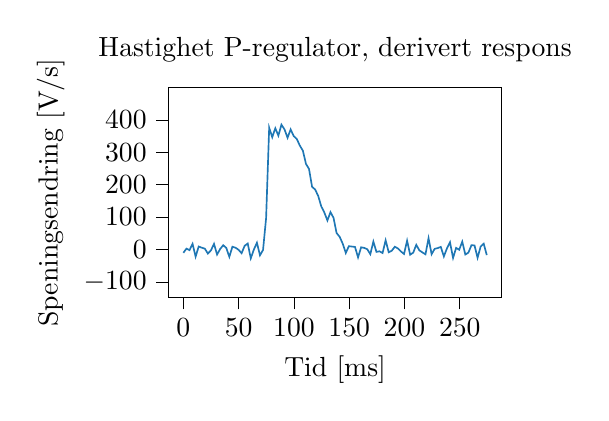
\begin{tikzpicture}

\definecolor{darkgray176}{RGB}{176,176,176}
\definecolor{darkorange25512714}{RGB}{255,127,14}
\definecolor{steelblue31119180}{RGB}{31,119,180}

\begin{axis}[
tick align=outside,
tick pos=left,
title={Hastighet P-regulator, derivert respons},
%legend style={at={(0.95, 0.85)}, anchor=north east},
height=\figH,
width=\figW,
x grid style={darkgray176},
xlabel={Tid [ms]},
xmin=-13.7214000000001, xmax=288.149400000001,
xtick style={color=black},
xtick={-50,0,50,100,150,200,250,300},
xticklabels={
  \(\displaystyle {\ensuremath{-}50}\),
  \(\displaystyle {0}\),
  \(\displaystyle {50}\),
  \(\displaystyle {100}\),
  \(\displaystyle {150}\),
  \(\displaystyle {200}\),
  \(\displaystyle {250}\),
  \(\displaystyle {300}\)
},
y grid style={darkgray176},
ylabel={Speningsendring [V/s]},
ymin=-148.536402583333, ymax=498.70728425,
ytick style={color=black},
ytick={-200,-100,0,100,200,300,400,500},
yticklabels={
  \(\displaystyle {\ensuremath{-}200}\),
  \(\displaystyle {\ensuremath{-}100}\),
  \(\displaystyle {0}\),
  \(\displaystyle {100}\),
  \(\displaystyle {200}\),
  \(\displaystyle {300}\),
  \(\displaystyle {400}\),
  \(\displaystyle {500}\)
}
]
%\legend{$\omega_m$}
\addplot [semithick, steelblue31119180]
table {%
0 -10.5692640692493
2.77200000000377 2.34884559884681
5.54400000000221 -2.34884559884542
8.31600000000154 17.0277777777817
11.0880000000009 -22.3119288119061
13.8600000000038 8.80699855700101
16.6320000000031 5.28487253487567
19.4040000000015 2.34836459836575
22.176 -12.9175084174906
24.9480000000037 -2.93530543530631
27.7200000000031 17.0272967773061
30.4920000000015 -15.8537758537848
33.264 1.17460317460171
36.0360000000037 12.9173881673913
38.8080000000031 4.6972101972117
41.5800000000024 -22.8991101491306
44.3519999999999 8.22029822028706
47.1240000000037 5.28439153439121
49.8960000000039 -1.17412217412354
52.6680000000024 -11.7430254930314
55.4400000000008 11.1558441558286
58.2120000000046 18.2018999519113
60.984000000003 -27.5965608465681
63.7560000000024 -0.587301587302625
66.5280000000008 20.550745550718
69.3000000000046 -18.2020202020306
72.072000000003 -1.76118326118314
74.8440000000024 96.8809523810068
77.6160000000008 375.781866281716
80.3880000000019 346.423280423142
83.160000000003 374.020562770653
85.9320000000023 351.120610870808
88.7040000000008 385.176286676256
91.476000000001 370.497354497088
94.248000000003 344.662205387289
97.0200000000023 370.497163299753
99.7920000000017 349.946848244433
102.564000000001 341.138973063618
105.336000000004 320.588985089063
108.108000000003 304.73508898526
110.880000000002 264.221380471529
113.652 248.368446368108
116.424000000004 193.174963925011
119.196000000003 184.955387205491
121.968000000002 164.991702741743
124.740000000001 132.697570947433
127.512000000004 113.908609908638
130.284000000003 89.2490379990877
133.056000000002 115.08285233288
135.828000000001 97.4677729676719
138.600000000004 50.4956709956995
141.372000000002 38.7527657527633
144.144000000003 17.614598364608
146.916000000001 -11.1558441558292
149.688000000005 9.98196248196828
152.460000000003 8.80711880712096
155.232000000002 7.63287638288093
158.004000000001 -24.660413660388
160.776000000004 6.45851370851479
163.548000000003 4.69733044733164
166.320000000002 0.587181337182037
169.092000000001 -14.6790524290474
171.864000000002 24.0734728234635
174.636000000003 -7.6327561327579
177.408000000002 -5.87193362193712
180.180000000001 -11.1558441558429
182.952000000001 28.1839826839615
185.724000000003 -8.8074795574808
188.496000000002 -4.11026936027038
191.268000000002 8.2200577200597
194.040000000001 2.93590668590386
196.812000000003 -6.4588744588732
199.584000000003 -14.0918710918795
202.356000000002 27.0094997595149
205.128 -16.4405964405735
207.900000000004 -9.98160173160396
210.672000000003 14.0918710918789
213.444000000002 -2.93566618566837
216.216 -9.39430014428712
218.988000000004 -15.2665945165985
221.760000000003 34.6422558922759
224.532000000002 -14.6784511784545
227.304000000001 1.76130351130147
230.076000000004 4.10978835979063
232.848000000002 7.63299663299599
235.620000000003 -21.7247474747598
238.392000000001 2.93554593554308
241.164000000004 22.3122895622952
243.936000000003 -26.4219576719645
246.708000000003 4.69708994709326
249.480000000001 -1.17424242424161
252.252000000004 24.0732323232384
255.024000000003 -15.8531746031794
257.796000000003 -9.98172198172711
260.568000000001 12.9176286676236
263.340000000002 12.3302068302055
266.112000000002 -25.8346560846538
268.884000000003 8.80723905724437
271.656000000001 17.6147186147167
274.428000000001 -17.6147186147117
};
\end{axis}

\end{tikzpicture}

    \caption{
        Akselerasjonen til motoren under en sprangrespons, når motoren er regulert med en P-regulator for hastighet.
        Dataen har blitt lavpassfiltrert og er hentet fra \cite{EksempelData}.
    }.
    \label{fig:hastighet_P_regulator_derivert}
    \todo[inline]{denne figuren er vanskelig å tolke}
\end{figure}

\begin{figure}[h]
    \centering
    % This file was created with tikzplotlib v0.10.1.
% Dette er eksempel data
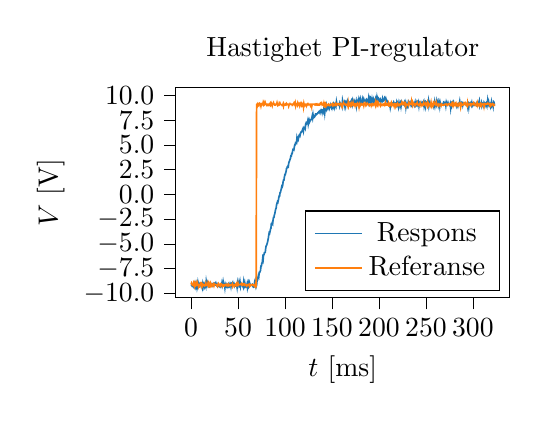
\begin{tikzpicture}

\definecolor{darkgray176}{RGB}{176,176,176}
\definecolor{darkorange25512714}{RGB}{255,127,14}
\definecolor{steelblue31119180}{RGB}{31,119,180}

\begin{axis}[
tick align=outside,
tick pos=left,
title={Hastighet PI-regulator},
legend pos=south east,
height=\figH,
width=\figW,
x grid style={darkgray176},
xlabel={\(\displaystyle t\) [ms]},
xmin=-16.1469, xmax=339.0849,
xtick style={color=black},
xtick={-50,0,50,100,150,200,250,300,350},
xticklabels={
  \(\displaystyle {\ensuremath{-}50}\),
  \(\displaystyle {0}\),
  \(\displaystyle {50}\),
  \(\displaystyle {100}\),
  \(\displaystyle {150}\),
  \(\displaystyle {200}\),
  \(\displaystyle {250}\),
  \(\displaystyle {300}\),
  \(\displaystyle {350}\)
},
y grid style={darkgray176},
ylabel={\(\displaystyle V\) [V]},
ymin=-10.410154, ymax=10.751954,
ytick style={color=black},
ytick={-12.5,-10,-7.5,-5,-2.5,0,2.5,5,7.5,10,12.5},
yticklabels={
  \(\displaystyle {\ensuremath{-}12.5}\),
  \(\displaystyle {\ensuremath{-}10.0}\),
  \(\displaystyle {\ensuremath{-}7.5}\),
  \(\displaystyle {\ensuremath{-}5.0}\),
  \(\displaystyle {\ensuremath{-}2.5}\),
  \(\displaystyle {0.0}\),
  \(\displaystyle {2.5}\),
  \(\displaystyle {5.0}\),
  \(\displaystyle {7.5}\),
  \(\displaystyle {10.0}\),
  \(\displaystyle {12.5}\)
}
]
\legend {Respons, Referanse}
\addplot [semithick, steelblue31119180]
table {%
0 -9.2041
0.46199999999974 -9.15527
0.923999999999925 -9.2041
1.38600000000011 -9.30176
1.84799999999985 -9.30176
2.31000000000003 -9.10645
2.77199999999977 -9.25293
3.23399999999996 -9.10645
3.69600000000014 -9.30176
4.15799999999988 -9.39941
4.62000000000007 -9.00879
5.08199999999981 -9.15527
5.54399999999999 -9.30176
6.00600000000018 -9.10645
6.46799999999992 -9.44824
6.9300000000001 -9.25293
7.39199999999984 -8.8623
7.85400000000003 -9.05762
8.31599999999977 -9.10645
8.77799999999995 -9.25293
9.24000000000014 -9.30176
9.70199999999988 -9.00879
10.1640000000001 -9.05762
10.6259999999998 -9.05762
11.088 -9.10645
11.5500000000002 -9.2041
12.0119999999999 -9.39941
12.4740000000001 -9.05762
12.9359999999998 -9.30176
13.398 -9.05762
13.8599999999998 -9.15527
14.3219999999999 -9.30176
14.7840000000001 -9.05762
15.2459999999999 -9.15527
15.7080000000001 -9.30176
16.1699999999998 -8.76465
16.632 -9.00879
17.0940000000002 -9.15527
17.5559999999999 -8.95996
18.0180000000001 -9.15527
18.4799999999998 -9.15527
18.942 -9.15527
19.4039999999998 -9.25293
19.8659999999999 -9.10645
20.3280000000001 -9.2041
20.7899999999999 -9.10645
21.252 -9.05762
21.7139999999998 -9.2041
22.176 -9.2041
22.6380000000002 -9.10645
23.0999999999999 -9.2041
23.5620000000001 -9.05762
24.0239999999998 -9.00879
24.486 -9.10645
24.9479999999997 -9.00879
25.4099999999999 -8.95996
25.8720000000001 -9.05762
26.3339999999999 -8.95996
26.796 -9.15527
27.2579999999998 -9.2041
27.72 -9.10645
28.1820000000002 -9.25293
28.6439999999999 -9.15527
29.1060000000001 -9.15527
29.5679999999998 -9.25293
30.03 -9.30176
30.4919999999997 -9.30176
30.9539999999999 -9.35059
31.4160000000001 -9.25293
31.8779999999999 -9.30176
32.34 -9.30176
32.8019999999998 -9.00879
33.264 -9.25293
33.7260000000001 -9.10645
34.1879999999999 -8.81348
34.6500000000001 -9.05762
35.1119999999998 -9.10645
35.574 -9.15527
36.0360000000002 -9.44824
36.4979999999999 -9.10645
36.9600000000001 -9.25293
37.4219999999998 -9.30176
37.884 -9.15527
38.3459999999998 -9.30176
38.808 -9.2041
39.2700000000001 -9.10645
39.7319999999999 -9.35059
40.1940000000001 -9.30176
40.6559999999998 -9.10645
41.118 -9.25293
41.5800000000002 -9.15527
42.0419999999999 -9.05762
42.5040000000001 -9.30176
42.9659999999998 -9.00879
43.428 -9.05762
43.8899999999998 -9.00879
44.3519999999999 -8.91113
44.8140000000001 -9.15527
45.2759999999999 -9.15527
45.7380000000001 -9.05762
46.1999999999998 -9.25293
46.662 -9.15527
47.1240000000002 -9.25293
47.5859999999999 -9.25293
48.0480000000001 -9.15527
48.5099999999998 -9.15527
48.972 -9.39941
49.4339999999998 -8.95996
49.8959999999999 -9.2041
50.3580000000001 -9.2041
50.8199999999999 -8.95996
51.2820000000001 -9.30176
51.7439999999998 -9.25293
52.206 -8.91113
52.6680000000002 -9.25293
53.1299999999999 -9.00879
53.5920000000001 -9.10645
54.0539999999998 -9.10645
54.516 -9.15527
54.9779999999998 -9.25293
55.4399999999999 -9.35059
55.9020000000001 -8.95996
56.3639999999999 -9.39941
56.826 -9.30176
57.2879999999998 -9.00879
57.75 -9.30176
58.2120000000002 -9.35059
58.6739999999999 -9.30176
59.1360000000001 -9.25293
59.5979999999998 -9.05762
60.06 -9.44824
60.5219999999997 -9.25293
60.9839999999999 -9.00879
61.4460000000001 -9.30176
61.9079999999999 -9.2041
62.37 -8.95996
62.8319999999998 -9.15527
63.294 -9.10645
63.7560000000001 -9.10645
64.2179999999999 -9.15527
64.6800000000001 -9.15527
65.1419999999998 -9.10645
65.604 -9.30176
66.0660000000002 -9.30176
66.5279999999999 -9.35059
66.9900000000001 -9.30176
67.4519999999998 -9.00879
67.914 -9.30176
68.3759999999998 -9.35059
68.838 -8.95996
69.3000000000001 -9.30176
69.7619999999999 -9.15527
70.2240000000001 -8.71582
70.6859999999998 -8.66699
71.148 -8.42285
71.6100000000002 -8.22754
72.0719999999999 -8.3252
72.5340000000001 -7.88574
72.9959999999998 -7.88574
73.458 -7.78809
73.9199999999998 -7.69043
74.3819999999999 -7.25098
74.8440000000001 -7.25098
75.3059999999999 -6.95801
75.7680000000001 -6.90918
76.2299999999998 -6.46973
76.692 -6.61621
77.1540000000002 -6.12793
77.6159999999999 -6.0791
78.0780000000001 -5.88379
78.5399999999998 -5.88379
79.002 -5.83496
79.4639999999998 -5.44434
79.9259999999999 -5.2002
80.3880000000001 -5.15137
80.8499999999999 -5.00488
81.3120000000001 -4.8584
81.7739999999998 -4.66309
82.236 -4.41895
82.6980000000002 -4.12598
83.1599999999999 -3.88184
83.6220000000001 -3.93066
84.0839999999998 -3.73535
84.546 -3.49121
85.0079999999998 -3.44238
85.4699999999999 -2.9541
85.9320000000001 -2.9541
86.3939999999999 -2.85645
86.8560000000001 -2.9541
87.3179999999998 -2.56348
87.78 -2.31934
88.2420000000002 -2.31934
88.7039999999999 -2.0752
89.1660000000001 -1.92871
89.6279999999998 -1.68457
90.09 -1.48926
90.5519999999997 -1.3916
91.0139999999999 -1.0498
91.4760000000001 -0.90332
91.9379999999998 -0.756836
92.4 -0.805664
92.8619999999998 -0.610352
93.324 -0.366211
93.7860000000001 -0.170898
94.2479999999999 -0.170898
94.7100000000001 0.170898
95.1719999999998 0.219727
95.634 0.415039
96.0960000000002 0.561523
96.5579999999999 0.805664
97.0200000000001 0.756836
97.4819999999998 0.90332
97.944 1.24512
98.4059999999998 1.44043
98.868 1.44043
99.3300000000001 1.7334
99.7919999999999 1.97754
100.254 1.97754
100.716 2.17285
101.178 2.31934
101.64 2.6123
102.102 2.66113
102.564 2.80762
103.026 2.85645
103.488 2.80762
103.95 3.14941
104.412 3.2959
104.874 3.39355
105.336 3.54004
105.798 3.6377
106.26 3.88184
106.722 3.88184
107.184 4.12598
107.646 4.12598
108.108 4.37012
108.57 4.56543
109.032 4.56543
109.494 4.5166
109.956 4.80957
110.418 5.00488
110.88 5.00488
111.342 5.24902
111.804 5.24902
112.266 5.2002
112.728 5.68848
113.19 5.49316
113.652 5.63965
114.114 5.54199
114.576 5.78613
115.038 5.98145
115.5 6.03027
115.962 5.93262
116.424 6.12793
116.886 6.27441
117.348 6.27441
117.81 6.32324
118.272 6.4209
118.734 6.56738
119.196 6.66504
119.658 6.4209
120.12 6.71387
120.582 6.71387
121.044 6.7627
121.506 6.66504
121.968 7.10449
122.43 7.20215
122.892 7.10449
123.354 7.15332
123.816 7.25098
124.278 7.44629
124.74 7.10449
125.202 7.34863
125.664 7.49512
126.126 7.2998
126.588 7.39746
127.05 7.49512
127.512 7.54395
127.974 7.54395
128.436 7.69043
128.898 7.88574
129.36 7.69043
129.822 8.03223
130.284 7.73926
130.746 7.78809
131.208 7.78809
131.67 7.93457
132.132 7.93457
132.594 8.12988
133.056 8.12988
133.518 8.08105
133.98 8.12988
134.442 8.12988
134.904 8.22754
135.366 8.22754
135.828 8.3252
136.29 8.37402
136.752 8.3252
137.214 8.22754
137.676 8.42285
138.138 8.37402
138.6 8.52051
139.062 8.47168
139.524 8.27637
139.986 8.52051
140.448 8.52051
140.91 8.37402
141.372 8.66699
141.834 8.61816
142.296 8.22754
142.758 8.61816
143.22 8.76465
143.682 8.66699
144.144 8.91113
144.606 8.56934
145.068 8.66699
145.53 8.8623
145.992 8.76465
146.454 8.71582
146.916 8.61816
147.378 8.81348
147.84 8.81348
148.302 9.00879
148.764 8.8623
149.226 8.76465
149.688 8.91113
150.15 8.71582
150.612 8.8623
151.074 8.91113
151.536 8.81348
151.998 9.2041
152.46 9.15527
152.922 8.8623
153.384 9.10645
153.846 9.10645
154.308 8.95996
154.77 9.35059
155.232 9.10645
155.694 9.10645
156.156 9.10645
156.618 9.05762
157.08 9.10645
157.542 9.15527
158.004 8.95996
158.466 9.25293
158.928 9.15527
159.39 9.05762
159.852 9.15527
160.314 9.15527
160.776 8.95996
161.238 9.49707
161.7 9.30176
162.162 9.25293
162.624 9.30176
163.086 9.00879
163.548 9.30176
164.01 9.2041
164.472 8.95996
164.934 9.35059
165.396 9.30176
165.858 9.2041
166.32 9.39941
166.782 9.2041
167.244 9.2041
167.706 9.30176
168.168 9.15527
168.63 9.30176
169.092 9.30176
169.554 9.10645
170.016 9.35059
170.478 9.44824
170.94 9.25293
171.402 9.39941
171.864 9.15527
172.326 9.49707
172.788 9.35059
173.25 9.35059
173.712 9.35059
174.174 9.44824
174.636 9.2041
175.098 9.35059
175.56 9.39941
176.022 9.00879
176.484 9.39941
176.946 9.2041
177.408 9.15527
177.87 9.35059
178.332 9.15527
178.794 9.59473
179.256 9.44824
179.718 9.35059
180.18 9.59473
180.642 9.35059
181.104 9.44824
181.566 9.44824
182.028 9.30176
182.49 9.64355
182.952 9.49707
183.414 9.39941
183.876 9.59473
184.338 9.44824
184.8 9.49707
185.262 9.49707
185.724 9.39941
186.186 9.49707
186.648 9.30176
187.11 9.35059
187.572 9.5459
188.034 9.49707
188.496 9.30176
188.958 9.64355
189.42 9.30176
189.882 9.39941
190.344 9.64355
190.806 9.44824
191.268 9.64355
191.73 9.49707
192.192 9.30176
192.654 9.59473
193.116 9.35059
193.578 9.35059
194.04 9.5459
194.502 9.30176
194.964 9.49707
195.426 9.39941
195.888 9.35059
196.35 9.59473
196.812 9.39941
197.274 9.49707
197.736 9.79004
198.198 9.49707
198.66 9.74121
199.122 9.64355
199.584 9.39941
200.046 9.59473
200.508 9.49707
200.97 9.44824
201.432 9.5459
201.894 9.30176
202.356 9.39941
202.818 9.49707
203.28 9.44824
203.742 9.64355
204.204 9.39941
204.666 9.44824
205.128 9.59473
205.59 9.59473
206.052 9.74121
206.514 9.64355
206.976 9.44824
207.438 9.64355
207.9 9.49707
208.362 9.49707
208.824 9.39941
209.286 9.2041
209.748 9.10645
210.21 9.15527
210.672 9.05762
211.134 8.95996
211.596 9.05762
212.058 8.76465
212.52 9.00879
212.982 9.10645
213.444 9.05762
213.906 9.2041
214.368 9.15527
214.83 9.10645
215.292 9.15527
215.754 9.30176
216.216 9.2041
216.678 9.10645
217.14 9.00879
217.602 9.15527
218.064 9.10645
218.526 9.00879
218.988 9.30176
219.45 9.15527
219.912 9.00879
220.374 9.2041
220.836 8.91113
221.298 9.25293
221.76 9.25293
222.222 9.05762
222.684 9.39941
223.146 9.35059
223.608 8.95996
224.07 9.25293
224.532 9.10645
224.994 9.15527
225.456 9.10645
225.918 9.15527
226.38 9.05762
226.842 9.00879
227.304 9.25293
227.766 9.10645
228.228 9.25293
228.69 8.81348
229.152 9.10645
229.614 8.95996
230.076 8.8623
230.538 9.05762
231 9.25293
231.462 9.05762
231.924 9.35059
232.386 9.30176
232.848 9.25293
233.31 9.25293
233.772 9.10645
234.234 9.35059
234.696 9.30176
235.158 8.95996
235.62 9.00879
236.082 9.15527
236.544 9.10645
237.006 9.15527
237.468 9.00879
237.93 9.15527
238.392 9.30176
238.854 8.91113
239.316 8.95996
239.778 9.15527
240.24 9.05762
240.702 9.39941
241.164 9.35059
241.626 9.15527
242.088 9.30176
242.55 8.95996
243.012 9.30176
243.474 9.25293
243.936 9.00879
244.398 9.00879
244.86 9.2041
245.322 9.05762
245.784 9.05762
246.246 9.2041
246.708 9.10645
247.17 9.30176
247.632 9.39941
248.094 8.95996
248.556 9.2041
249.018 9.05762
249.48 8.8623
249.942 9.35059
250.404 9.30176
250.866 9.30176
251.328 9.25293
251.79 9.25293
252.252 9.10645
252.714 9.39941
253.176 8.95996
253.638 9.2041
254.1 9.30176
254.562 9.10645
255.024 9.00879
255.486 9.10645
255.948 9.10645
256.41 9.10645
256.872 9.10645
257.334 9.05762
257.796 9.10645
258.258 8.91113
258.72 9.10645
259.182 9.35059
259.644 9.00879
260.106 9.30176
260.568 9.30176
261.03 9.10645
261.492 9.39941
261.954 9.15527
262.416 9.2041
262.878 9.35059
263.34 8.95996
263.802 9.10645
264.264 9.25293
264.726 8.91113
265.188 9.25293
265.65 9.05762
266.112 9.10645
266.574 9.05762
267.036 9.00879
267.498 9.00879
267.96 9.10645
268.422 9.2041
268.884 9.10645
269.346 9.25293
269.808 9.15527
270.27 9.2041
270.732 9.25293
271.194 8.95996
271.656 9.30176
272.118 9.15527
272.58 9.10645
273.042 9.10645
273.504 9.25293
273.966 9.10645
274.428 9.10645
274.89 9.10645
275.352 9.00879
275.814 9.15527
276.276 8.76465
276.738 9.2041
277.2 9.25293
277.662 9.00879
278.124 9.2041
278.586 9.30176
279.048 9.10645
279.51 9.25293
279.972 9.05762
280.434 9.10645
280.896 9.10645
281.358 9.05762
281.82 9.15527
282.282 9.15527
282.744 8.95996
283.206 9.15527
283.668 9.15527
284.13 8.95996
284.592 9.15527
285.054 9.2041
285.516 9.15527
285.978 9.39941
286.44 9.10645
286.902 9.10645
287.364 9.15527
287.826 9.2041
288.288 9.30176
288.75 9.25293
289.212 9.00879
289.674 9.2041
290.136 9.2041
290.598 9.15527
291.06 9.15527
291.522 9.10645
291.984 9.2041
292.446 9.15527
292.908 9.05762
293.37 9.05762
293.832 9.15527
294.294 8.91113
294.756 9.30176
295.218 9.30176
295.68 8.8623
296.142 9.2041
296.604 9.2041
297.066 9.2041
297.528 9.25293
297.99 9.05762
298.452 8.95996
298.914 9.2041
299.376 8.95996
299.838 9.05762
300.3 9.15527
300.762 9.05762
301.224 9.15527
301.686 9.2041
302.148 9.05762
302.61 9.10645
303.072 9.05762
303.534 9.00879
303.996 9.25293
304.458 9.30176
304.92 9.2041
305.382 9.10645
305.844 9.05762
306.306 9.30176
306.768 9.44824
307.23 8.95996
307.692 9.10645
308.154 9.00879
308.616 9.00879
309.078 9.2041
309.54 8.91113
310.002 9.05762
310.464 9.15527
310.926 9.10645
311.388 8.95996
311.85 9.25293
312.312 9.15527
312.774 9.2041
313.236 9.15527
313.698 9.00879
314.16 9.25293
314.622 9.30176
315.084 9.05762
315.546 9.39941
316.008 8.95996
316.47 8.95996
316.932 9.25293
317.394 9.00879
317.856 9.10645
318.318 9.15527
318.78 8.8623
319.242 9.00879
319.704 9.30176
320.166 9.00879
320.628 9.15527
321.09 9.15527
321.552 8.91113
322.014 9.35059
322.476 9.30176
322.938 8.95996
};
\addplot [semithick, darkorange25512714]
table {%
0 -9.05762
0.46199999999974 -8.95996
0.923999999999925 -9.10645
1.38600000000011 -9.15527
1.84799999999985 -9.10645
2.31000000000003 -9.15527
2.77199999999977 -8.95996
3.23399999999996 -9.10645
3.69600000000014 -9.25293
4.15799999999988 -8.95996
4.62000000000007 -9.05762
5.08199999999981 -9.15527
5.54399999999999 -8.95996
6.00600000000018 -9.15527
6.46799999999992 -9.15527
6.9300000000001 -8.95996
7.39199999999984 -9.10645
7.85400000000003 -9.30176
8.31599999999977 -9.15527
8.77799999999995 -9.15527
9.24000000000014 -9.25293
9.70199999999988 -9.15527
10.1640000000001 -8.95996
10.6259999999998 -9.00879
11.088 -8.95996
11.5500000000002 -9.25293
12.0119999999999 -9.10645
12.4740000000001 -9.2041
12.9359999999998 -9.10645
13.398 -9.15527
13.8599999999998 -9.15527
14.3219999999999 -9.2041
14.7840000000001 -9.10645
15.2459999999999 -9.10645
15.7080000000001 -8.95996
16.1699999999998 -9.15527
16.632 -9.10645
17.0940000000002 -9.10645
17.5559999999999 -9.15527
18.0180000000001 -8.95996
18.4799999999998 -9.15527
18.942 -9.00879
19.4039999999998 -9.2041
19.8659999999999 -9.10645
20.3280000000001 -9.2041
20.7899999999999 -8.95996
21.252 -9.05762
21.7139999999998 -9.2041
22.176 -9.10645
22.6380000000002 -9.15527
23.0999999999999 -9.2041
23.5620000000001 -9.05762
24.0239999999998 -9.00879
24.486 -9.2041
24.9479999999997 -9.05762
25.4099999999999 -9.05762
25.8720000000001 -9.10645
26.3339999999999 -9.10645
26.796 -9.10645
27.2579999999998 -9.15527
27.72 -9.25293
28.1820000000002 -9.30176
28.6439999999999 -9.10645
29.1060000000001 -9.00879
29.5679999999998 -9.10645
30.03 -9.10645
30.4919999999997 -9.2041
30.9539999999999 -9.25293
31.4160000000001 -9.05762
31.8779999999999 -9.10645
32.34 -9.05762
32.8019999999998 -9.15527
33.264 -9.25293
33.7260000000001 -9.10645
34.1879999999999 -9.10645
34.6500000000001 -9.25293
35.1119999999998 -9.25293
35.574 -9.10645
36.0360000000002 -9.10645
36.4979999999999 -9.15527
36.9600000000001 -9.10645
37.4219999999998 -9.15527
37.884 -9.10645
38.3459999999998 -9.2041
38.808 -9.10645
39.2700000000001 -9.10645
39.7319999999999 -9.05762
40.1940000000001 -9.2041
40.6559999999998 -9.15527
41.118 -9.15527
41.5800000000002 -9.2041
42.0419999999999 -9.10645
42.5040000000001 -9.10645
42.9659999999998 -9.10645
43.428 -9.15527
43.8899999999998 -9.05762
44.3519999999999 -9.25293
44.8140000000001 -9.10645
45.2759999999999 -9.10645
45.7380000000001 -9.15527
46.1999999999998 -9.25293
46.662 -9.15527
47.1240000000002 -9.10645
47.5859999999999 -9.05762
48.0480000000001 -9.15527
48.5099999999998 -9.00879
48.972 -9.10645
49.4339999999998 -9.15527
49.8959999999999 -8.95996
50.3580000000001 -9.15527
50.8199999999999 -9.10645
51.2820000000001 -9.10645
51.7439999999998 -9.10645
52.206 -9.10645
52.6680000000002 -9.10645
53.1299999999999 -9.05762
53.5920000000001 -9.10645
54.0539999999998 -9.00879
54.516 -9.10645
54.9779999999998 -9.15527
55.4399999999999 -9.10645
55.9020000000001 -9.00879
56.3639999999999 -9.00879
56.826 -9.15527
57.2879999999998 -9.10645
57.75 -9.10645
58.2120000000002 -9.10645
58.6739999999999 -9.2041
59.1360000000001 -9.25293
59.5979999999998 -9.10645
60.06 -9.10645
60.5219999999997 -9.15527
60.9839999999999 -9.10645
61.4460000000001 -9.15527
61.9079999999999 -9.10645
62.37 -9.30176
62.8319999999998 -9.25293
63.294 -9.15527
63.7560000000001 -9.10645
64.2179999999999 -9.10645
64.6800000000001 -9.10645
65.1419999999998 -9.15527
65.604 -9.10645
66.0660000000002 -9.15527
66.5279999999999 -9.15527
66.9900000000001 -9.2041
67.4519999999998 -9.25293
67.914 -9.15527
68.3759999999998 -9.25293
68.838 -9.00879
69.3000000000001 -9.10645
69.7619999999999 9.05762
70.2240000000001 9.10645
70.6859999999998 8.95996
71.148 9.10645
71.6100000000002 9.00879
72.0719999999999 8.95996
72.5340000000001 9.15527
72.9959999999998 9.2041
73.458 9.15527
73.9199999999998 9.10645
74.3819999999999 8.91113
74.8440000000001 9.10645
75.3059999999999 9.15527
75.7680000000001 9.10645
76.2299999999998 9.05762
76.692 9.25293
77.1540000000002 9.10645
77.6159999999999 9.25293
78.0780000000001 9.05762
78.5399999999998 9.10645
79.002 9.25293
79.4639999999998 9.10645
79.9259999999999 9.05762
80.3880000000001 9.00879
80.8499999999999 9.10645
81.3120000000001 9.10645
81.7739999999998 8.95996
82.236 8.95996
82.6980000000002 9.05762
83.1599999999999 9.10645
83.6220000000001 9.05762
84.0839999999998 9.15527
84.546 8.95996
85.0079999999998 9.00879
85.4699999999999 9.2041
85.9320000000001 9.10645
86.3939999999999 8.95996
86.8560000000001 9.15527
87.3179999999998 9.15527
87.78 9.25293
88.2420000000002 9.10645
88.7039999999999 9.10645
89.1660000000001 9.00879
89.6279999999998 9.00879
90.09 9.05762
90.5519999999997 9.10645
91.0139999999999 9.10645
91.4760000000001 9.25293
91.9379999999998 9.05762
92.4 8.95996
92.8619999999998 9.00879
93.324 9.05762
93.7860000000001 9.2041
94.2479999999999 9.10645
94.7100000000001 9.2041
95.1719999999998 9.10645
95.634 9.05762
96.0960000000002 9.05762
96.5579999999999 9.05762
97.0200000000001 8.95996
97.4819999999998 8.95996
97.944 9.10645
98.4059999999998 8.91113
98.868 9.10645
99.3300000000001 9.00879
99.7919999999999 9.00879
100.254 9.00879
100.716 9.10645
101.178 9.05762
101.64 9.15527
102.102 9.05762
102.564 9.05762
103.026 9.10645
103.488 9.10645
103.95 8.91113
104.412 9.05762
104.874 9.05762
105.336 9.15527
105.798 9.10645
106.26 9.10645
106.722 9.10645
107.184 9.10645
107.646 9.00879
108.108 9.05762
108.57 9.10645
109.032 9.10645
109.494 9.2041
109.956 9.05762
110.418 9.10645
110.88 9.25293
111.342 8.95996
111.804 9.15527
112.266 9.15527
112.728 9.10645
113.19 9.00879
113.652 9.25293
114.114 9.15527
114.576 9.05762
115.038 9.10645
115.5 8.95996
115.962 9.15527
116.424 9.10645
116.886 9.2041
117.348 9.00879
117.81 9.10645
118.272 8.95996
118.734 9.00879
119.196 9.10645
119.658 8.81348
120.12 9.15527
120.582 8.95996
121.044 9.05762
121.506 9.00879
121.968 9.10645
122.43 9.10645
122.892 8.95996
123.354 9.10645
123.816 9.10645
124.278 9.15527
124.74 9.05762
125.202 9.10645
125.664 9.10645
126.126 9.05762
126.588 9.05762
127.05 8.95996
127.512 9.10645
127.974 9.10645
128.436 8.8623
128.898 9.10645
129.36 9.10645
129.822 9.10645
130.284 9.10645
130.746 9.10645
131.208 9.10645
131.67 9.05762
132.132 9.10645
132.594 9.05762
133.056 9.10645
133.518 9.05762
133.98 9.10645
134.442 9.00879
134.904 9.00879
135.366 9.10645
135.828 9.10645
136.29 9.00879
136.752 9.00879
137.214 9.15527
137.676 9.2041
138.138 9.10645
138.6 9.10645
139.062 9.2041
139.524 9.05762
139.986 9.10645
140.448 9.10645
140.91 9.00879
141.372 9.2041
141.834 9.00879
142.296 9.10645
142.758 8.95996
143.22 9.10645
143.682 8.95996
144.144 9.10645
144.606 9.05762
145.068 8.95996
145.53 8.95996
145.992 9.00879
146.454 9.10645
146.916 9.05762
147.378 9.00879
147.84 8.95996
148.302 9.05762
148.764 9.10645
149.226 9.10645
149.688 9.05762
150.15 9.00879
150.612 9.10645
151.074 8.95996
151.536 9.00879
151.998 9.10645
152.46 9.05762
152.922 8.95996
153.384 8.95996
153.846 9.10645
154.308 8.95996
154.77 8.95996
155.232 9.10645
155.694 9.05762
156.156 9.05762
156.618 9.15527
157.08 9.15527
157.542 9.15527
158.004 9.05762
158.466 9.10645
158.928 9.15527
159.39 9.05762
159.852 9.10645
160.314 8.95996
160.776 8.81348
161.238 8.95996
161.7 9.10645
162.162 9.25293
162.624 9.15527
163.086 9.15527
163.548 9.15527
164.01 9.05762
164.472 9.00879
164.934 9.00879
165.396 9.05762
165.858 9.10645
166.32 9.10645
166.782 8.95996
167.244 9.25293
167.706 8.91113
168.168 9.05762
168.63 9.00879
169.092 9.15527
169.554 9.05762
170.016 8.95996
170.478 9.15527
170.94 8.95996
171.402 9.00879
171.864 9.10645
172.326 9.25293
172.788 8.95996
173.25 8.95996
173.712 9.15527
174.174 9.15527
174.636 8.95996
175.098 9.10645
175.56 9.05762
176.022 9.10645
176.484 8.95996
176.946 9.00879
177.408 9.2041
177.87 9.15527
178.332 9.05762
178.794 8.81348
179.256 9.05762
179.718 8.91113
180.18 9.00879
180.642 9.00879
181.104 9.15527
181.566 9.10645
182.028 9.05762
182.49 9.10645
182.952 9.10645
183.414 9.15527
183.876 8.95996
184.338 9.15527
184.8 9.05762
185.262 9.05762
185.724 9.15527
186.186 8.95996
186.648 9.00879
187.11 9.05762
187.572 9.15527
188.034 9.05762
188.496 9.05762
188.958 9.10645
189.42 9.10645
189.882 9.00879
190.344 9.10645
190.806 9.10645
191.268 9.10645
191.73 8.95996
192.192 9.10645
192.654 9.15527
193.116 9.10645
193.578 9.00879
194.04 9.10645
194.502 9.10645
194.964 9.15527
195.426 9.10645
195.888 9.00879
196.35 9.25293
196.812 8.95996
197.274 9.10645
197.736 9.25293
198.198 9.10645
198.66 9.25293
199.122 9.05762
199.584 9.2041
200.046 9.10645
200.508 9.05762
200.97 9.05762
201.432 8.95996
201.894 9.10645
202.356 9.00879
202.818 9.05762
203.28 9.00879
203.742 9.10645
204.204 9.10645
204.666 9.05762
205.128 9.10645
205.59 9.00879
206.052 9.10645
206.514 9.05762
206.976 9.25293
207.438 9.10645
207.9 9.00879
208.362 9.00879
208.824 9.10645
209.286 9.05762
209.748 9.00879
210.21 9.2041
210.672 9.05762
211.134 8.95996
211.596 9.00879
212.058 9.15527
212.52 9.10645
212.982 9.00879
213.444 9.25293
213.906 9.15527
214.368 9.10645
214.83 9.00879
215.292 9.05762
215.754 9.10645
216.216 8.91113
216.678 9.10645
217.14 9.15527
217.602 9.15527
218.064 8.8623
218.526 8.95996
218.988 9.05762
219.45 9.00879
219.912 9.15527
220.374 9.05762
220.836 9.00879
221.298 9.10645
221.76 9.10645
222.222 9.00879
222.684 9.10645
223.146 9.05762
223.608 9.05762
224.07 9.05762
224.532 9.30176
224.994 9.2041
225.456 9.25293
225.918 9.05762
226.38 9.05762
226.842 9.10645
227.304 9.2041
227.766 9.00879
228.228 9.10645
228.69 8.91113
229.152 9.10645
229.614 9.10645
230.076 9.05762
230.538 9.10645
231 9.10645
231.462 9.00879
231.924 9.25293
232.386 9.10645
232.848 9.15527
233.31 9.10645
233.772 9.10645
234.234 9.10645
234.696 9.39941
235.158 9.15527
235.62 9.00879
236.082 9.25293
236.544 9.10645
237.006 9.2041
237.468 9.15527
237.93 9.15527
238.392 8.95996
238.854 9.05762
239.316 9.10645
239.778 9.15527
240.24 9.10645
240.702 9.25293
241.164 9.10645
241.626 9.10645
242.088 9.00879
242.55 8.95996
243.012 9.05762
243.474 9.10645
243.936 9.25293
244.398 9.15527
244.86 8.95996
245.322 9.05762
245.784 9.10645
246.246 9.10645
246.708 9.00879
247.17 9.10645
247.632 9.25293
248.094 9.10645
248.556 9.15527
249.018 9.15527
249.48 9.05762
249.942 9.2041
250.404 9.10645
250.866 9.10645
251.328 8.95996
251.79 9.2041
252.252 8.95996
252.714 9.10645
253.176 8.95996
253.638 9.00879
254.1 9.10645
254.562 9.15527
255.024 9.00879
255.486 9.25293
255.948 8.95996
256.41 9.10645
256.872 9.10645
257.334 8.95996
257.796 9.2041
258.258 9.10645
258.72 9.25293
259.182 9.10645
259.644 9.10645
260.106 9.15527
260.568 9.05762
261.03 9.30176
261.492 9.15527
261.954 9.10645
262.416 9.00879
262.878 8.95996
263.34 9.05762
263.802 8.95996
264.264 9.10645
264.726 9.10645
265.188 9.05762
265.65 9.05762
266.112 8.95996
266.574 9.10645
267.036 9.05762
267.498 9.05762
267.96 9.00879
268.422 9.00879
268.884 9.00879
269.346 9.00879
269.808 9.10645
270.27 9.10645
270.732 9.05762
271.194 9.05762
271.656 9.10645
272.118 9.05762
272.58 8.95996
273.042 8.95996
273.504 9.05762
273.966 9.15527
274.428 9.15527
274.89 9.10645
275.352 9.10645
275.814 9.10645
276.276 8.95996
276.738 8.95996
277.2 9.10645
277.662 9.2041
278.124 9.05762
278.586 9.15527
279.048 8.95996
279.51 9.10645
279.972 8.95996
280.434 8.95996
280.896 9.15527
281.358 9.2041
281.82 9.25293
282.282 9.00879
282.744 9.10645
283.206 9.10645
283.668 9.00879
284.13 9.10645
284.592 8.95996
285.054 9.00879
285.516 9.05762
285.978 9.15527
286.44 9.05762
286.902 8.81348
287.364 9.10645
287.826 9.00879
288.288 9.10645
288.75 9.00879
289.212 9.00879
289.674 9.05762
290.136 9.05762
290.598 9.2041
291.06 9.10645
291.522 9.10645
291.984 9.2041
292.446 9.10645
292.908 9.00879
293.37 9.05762
293.832 8.95996
294.294 9.25293
294.756 9.00879
295.218 9.10645
295.68 9.10645
296.142 9.10645
296.604 9.05762
297.066 9.15527
297.528 9.10645
297.99 9.00879
298.452 9.15527
298.914 9.15527
299.376 9.10645
299.838 9.05762
300.3 9.05762
300.762 9.2041
301.224 9.10645
301.686 9.15527
302.148 9.05762
302.61 8.95996
303.072 8.95996
303.534 9.10645
303.996 9.10645
304.458 9.25293
304.92 8.95996
305.382 9.05762
305.844 9.10645
306.306 9.00879
306.768 9.05762
307.23 8.95996
307.692 9.10645
308.154 9.00879
308.616 9.10645
309.078 8.95996
309.54 9.05762
310.002 9.10645
310.464 9.05762
310.926 9.05762
311.388 9.10645
311.85 8.8623
312.312 9.10645
312.774 9.05762
313.236 9.15527
313.698 9.15527
314.16 9.15527
314.622 9.10645
315.084 9.10645
315.546 9.10645
316.008 9.2041
316.47 9.15527
316.932 9.15527
317.394 9.15527
317.856 8.95996
318.318 8.91113
318.78 9.10645
319.242 9.05762
319.704 9.00879
320.166 9.10645
320.628 9.15527
321.09 9.10645
321.552 9.10645
322.014 8.95996
322.476 9.00879
322.938 9.15527
};
\end{axis}

\end{tikzpicture}

    \caption{Sprangresponsen til PI-regulatoren for hastighet. Dataen er hentet fra \cite{EksempelData}.}
    \label{fig:hastighet_PI_regulator}
\end{figure}






\todo[inline]{figurtekst på figur 5 er fucked}
\subsection{Diskusjon}

I \autoref{fig:hastighet_P_regulator} er det et tydelig stasjonæravvik, mellom responsen til regulatoren og referanseverdien. Det er flere årsaker til at stasjonæravviket oppstår, blant annet friksjon i motoren, giret, og potensiometeret. Dersom motoren bremses, vil det stasjonære avviket øke, til tross for at pådraget også vil øke. Observasjonene i seksjon \ref{obs:hastighet_regulator_breming_med_finger} viser også at dette stasjonæravviket vil øke dersom motoren bremses mer.

Til tross for at det er et stasjonæravvik er det ikke så stort. Dette kommer antageligvis av at $K_p$ er stor. Siden $K_p$ er stor kan dette føre til at pådraget til regulatoren går i metning. Dette vil føre til slew-rate i regulatoren. Dette kommer fram i \autoref{fig:hastighet_P_regulator_derivert}. I intervallet \SI{80}{\milli\second} til \SI{100}{\milli\second} er akselerasjonen til motoren konstant, altså er endringen til hastigheten begrenset.

PI-regulatoren oppnår stasjonærverdi, som vist i \autoref{fig:hastighet_PI_regulator} og sett i observasjonene i seksjon \ref{obs:hastighet_regulator_breming_med_finger}. Etter omtrent \SI{150}{\milli\second} er det er oversving, som viser at systemet er litt underdempet. 

% Sammenlign hvor følsom motorhastigheten er for ekstra belastning n˚ar vi bruker regulatorenkontra å styre motoren direkte slik dere gjorde i forrige uke
\input{posisjonsmåler}
\section{Posisjonsregulator}\label{sec:posisjonsregulator}

\subsection{Teori}

% Reguleringoversving
% Kaskaderegulator
% P-regulator
% Zenerdiode

En zenerdiode er en halvlederdiode som lar strøm gå både med og mot diodens sperreretning. 
Dioden er laget slik at det kreves en viss spenning for strøm skal kunne gå mot sperreretningen, denne spenningen kalles zenerspenningen.
En zenerdiode sørger derfor for at spenningen over seg ikke blir noe høyere enn zenerspenningen sin, og kan derfor brukes til å holde en konstant spenning lavere enn den forsynte spenningen\cite{Zenerdiode}.





\subsection{Metode}

\begin{figure} [h]
    \centering
    \begin{circuitikz} [scale=0.5, transform shape]
\ctikzset{resistor = european}

\node[op amp](OP1){$OP1$};

\draw (OP1.-)
    to[short,-*] ++(-0.5,0)
    coordinate(temp)
    to[R,l_=$R_6$] ++(-2,0)
    -- ++(-6,0)
    to[short,-o,l=$\theta_m$] ++(0,0);

\draw (temp)
    -- ++(0,1)
    coordinate(temp)
    to[R,l=$R_7$] (temp -| OP1.out)
    -- (OP1.out)
    to[short,*-] ++(1,0)
    node[op amp, noinv input up, anchor=+](OP2){$OP2$};

\draw (OP1.+)
    to[short,-*] ++(-0.5,0)
    coordinate(OP1out)
    to[R,l=$R_6$] ++(-2,0)
    --node[anchor=west, yshift=-1cm]{$\theta_d$} ++(0,-2)
    coordinate(potwiper)
    ++(-1,1)
    coordinate(pottop)
    to[potentiometer, l_=$R_4$, n=R4] ++(0,-2)
    to[R,l=$R_5$] ++(-2,0)
    to[short,-*] ++(0,0)
    coordinate(Cbot)
    to[short, -*] ++(-1,0)
    coordinate(zenerbot)
    node[ground]{};

\draw (pottop)
    to[R, l_=$R_3$] ++(-2,0)
    to[short, -*] ++(0,0)
    coordinate(Ctop)
    to[short,-*] ++(-1,0)
    coordinate(zenertop)
    to[R, l_=$R_2$] ++(-2,0)
    -- ++(0,1)
    to[short, -o, l=$+15V$] ++(0,0);

\draw (Ctop)
    to[C, l=$C_1$] (Cbot);
\draw (zenerbot)
    to[zzDo, l=$D1$] (zenertop);

\draw (potwiper)
    -- (R4.wiper);

\draw (OP1out)
    to[R, l=$R_7$] ++(0,-3)
    node[ground]{};

\draw (OP2.-)
    to[short,-*] ++(-0.5,0)
    coordinate(OP2+)
    -- ++(-0.5,0)
    to[R, l_=$R_8$] ++(0,-2)
    -- ++(0,-0.5)
    node[ground]{};

\draw (OP2.out)
    -- ++(0,-2)
    coordinate(temp)
    to[potentiometer, l_=$R_9$, n=R9] (temp -| OP2+)
    -- (OP2+);

\draw (temp)
    ++(-0.5,0)
    to[short,*-] ++(0,0)
    -- ++(0,-1)
    -| (R9.wiper);

\draw (OP2.out)
    to[short, *-] ++(0,0)
    -- ++(1,0)
    to[short, -o, l_=$\omega_d$] ++(0,0);
    

    
    
    
    





\end{circuitikz}
    \caption{Differensiell operasjonsforsterker. Figuren er hentet fra \cite{AnalogMotorlabbOppgaver}.}
    \label{fig:Posisjonsregulator}
\end{figure}

\begin{table}[h]
    \centering
    \caption{Komponenter i posisjonsregulatoren. Verdiene er hentet fra \cite{AnalogMotorlabbOppgaver}.}
    \begin{tabular}{lll}
        \toprule
		Størrelse & Verdi & Type \\
		\midrule
        $R_2$ & \SI{560}{\ohm} & Resistor \\
        $R_3$ & \SI{1.5}{\kilo\ohm} & Resistor\\
        $R_4$ & \SI{10}{\kilo\ohm} & Potmeter\\
        $R_5$ & \SI{5.6}{\kilo\ohm} & Resistor\\
        $R_6, R_7$ & \SI{100}{\kilo\ohm} & Resistor\\
        $R_8$ & \SI{27}{\kilo\ohm} & Resistor\\
        $R_9$ & \SI{10}{\mega\ohm} & Potmeter\\
        $D_1$ & \SI{5.1}{\volt} & Zenerdiode\\
        $C_1$ & \SI{100}{\nano\farad} & Kondensator\\
		\bottomrule
    \end{tabular}
    \label{tab:Posisjonsregulator}
\end{table}

Som siste del av prosjektet ble posisjonsregulatoren implementert. Kretsen er vist i \autoref{fig:Posisjonsregulator} og ble implementert med komponentene i \autoref{tab:Posisjonsregulator}. Posisjonsregulatoren er satt sammen av en krets for å gi en posisjonsreferanse $\theta_d$ og regulatoren selv.
Posisjonsreferansekretsen benytter en zenerdiode for å opprettholde en konstant referansespenning på {\SI{5.1}{\volt}} til en spenningsdeling over $R_3$, $R_4$ og $R_5$. 
Kondensatoren $C_1$, vil hjelpe til med å holde en jevnere spenning, og fjerne støy inn til spenningsdelingen. 
Posisjonsreferansen $\theta_d$ kunne dermed justeres ved å endre på potensiometeret $R_4$. Denne referansen ble så sendt inn i selve regulatoren. 
Ved bruk av spenningsdeling blir $\theta_d = \frac{x R_4 + R_5}{R_3 + R_4 + R_5} D1$, der $x$ er et tall fra 0 til 1, etter hvilken posisjon $R_4$ er i og $D1$ er spenningen over zenerdioden. 
Intervallet til $R_4$ blir <\SI{1.7}{\volt}, \SI{4.7}{\volt}>. 
Siden dette intervallet er litt mindre enn intervallet til $\theta_m$ vil små reguleringsoversving over eller under referansen ikke føre til at slepekontakten går over $\theta_{max}$ eller under $\theta_{min}$. Dette hindrer servomotoren fra å rotere hele runder.

Regulatoren ble implementert som vist i høyre del av \autoref{fig:Posisjonsregulator}. Første operasjonforsterker sammenligner posisjonsreferansen $\theta_m$ og den målte posisjonen fra posisjonsmåleren $\theta_d$, slik at avviket blir $e_{\theta} = \theta_d - \theta_m$. Den andre operasjonforsterkeren forsterker signalet med en forsterkning justert av potensiometeret $R_9$. Ut av posisjonsregulatoren sendes $\omega_d$ til hastighetsregulatoren som referanse.
Etter at systemet var finjustert riktig ved bruk av de forskjellige potensiometerene, ble en signalgenerator koblet til $\theta_d$ i stedet for referansekretsen. Med signalgeneratoren kunne systemets frekvensrespons testes.







\subsection{Resultater}


\begin{figure}[h!]
    \centering
    % This file was created with tikzplotlib v0.10.1.
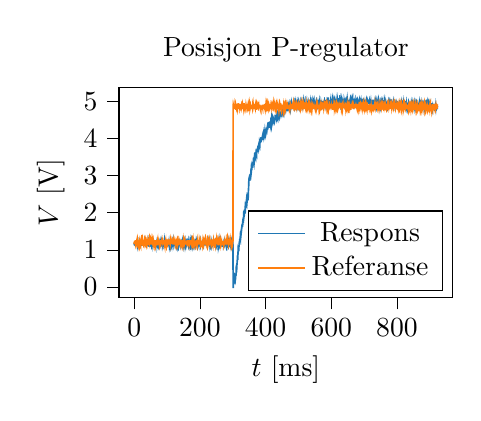
\begin{tikzpicture}

\definecolor{darkgray176}{RGB}{176,176,176}
\definecolor{darkorange25512714}{RGB}{255,127,14}
\definecolor{steelblue31119180}{RGB}{31,119,180}

\begin{axis}[
tick align=outside,
tick pos=left,
title={Posisjon P-regulator},
legend pos=south east,
height=\figH,
width=\figW,
x grid style={darkgray176},
xlabel={\(\displaystyle t\) [ms]},
xmin=-46.1769, xmax=969.714900000001,
xtick style={color=black},
xtick={-200,0,200,400,600,800,1000},
xticklabels={
  \(\displaystyle {\ensuremath{-}200}\),
  \(\displaystyle {0}\),
  \(\displaystyle {200}\),
  \(\displaystyle {400}\),
  \(\displaystyle {600}\),
  \(\displaystyle {800}\),
  \(\displaystyle {1000}\)
},
y grid style={darkgray176},
ylabel={\(\displaystyle V\) [V]},
ymin=-0.286132745, ymax=5.364255845,
ytick style={color=black},
ytick={-1,0,1,2,3,4,5,6},
yticklabels={
  \(\displaystyle {\ensuremath{-}1}\),
  \(\displaystyle {0}\),
  \(\displaystyle {1}\),
  \(\displaystyle {2}\),
  \(\displaystyle {3}\),
  \(\displaystyle {4}\),
  \(\displaystyle {5}\),
  \(\displaystyle {6}\)
}
]
\legend {Respons, Referanse}
\addplot [semithick, steelblue31119180]
table {%
0 1.14258
0.462000000000629 1.18164
0.924000000000369 1.12305
1.38600000000011 1.18164
1.84800000000074 1.18164
2.31000000000048 1.2207
2.77200000000022 1.16211
3.23400000000085 1.10352
3.69600000000059 1.2207
4.15800000000033 1.16211
4.62000000000007 1.20117
5.0820000000007 1.14258
5.54400000000044 1.14258
6.00600000000018 1.14258
6.46800000000081 1.14258
6.93000000000055 1.14258
7.39200000000029 1.14258
7.85400000000003 1.20117
8.31600000000066 1.12305
8.7780000000004 1.12305
9.24000000000014 1.20117
9.70200000000077 1.10352
10.1640000000005 1.2207
10.6260000000002 1.12305
11.0880000000009 1.14258
11.5500000000006 1.16211
12.0120000000004 1.2207
12.4740000000001 1.12305
12.9360000000007 1.20117
13.3980000000005 1.08398
13.8600000000002 1.20117
14.3220000000008 1.20117
14.7840000000006 1.12305
15.2460000000003 1.18164
15.7080000000001 1.16211
16.1700000000007 1.16211
16.6320000000004 1.16211
17.0940000000002 1.18164
17.5560000000008 1.14258
18.0180000000005 1.12305
18.4800000000003 1.14258
18.942 1.18164
19.4040000000006 1.2207
19.8660000000004 1.10352
20.3280000000001 1.20117
20.7900000000008 1.14258
21.2520000000005 1.14258
21.7140000000002 1.2207
22.1760000000009 1.2207
22.6380000000006 1.14258
23.1000000000003 1.10352
23.5620000000001 1.20117
24.0240000000007 1.20117
24.4860000000005 1.18164
24.9480000000002 1.18164
25.4100000000008 1.14258
25.8720000000006 1.14258
26.3340000000003 1.25977
26.796 1.2207
27.2580000000007 1.14258
27.7200000000004 1.25977
28.1820000000002 1.16211
28.6440000000008 1.12305
29.1060000000005 1.18164
29.5680000000003 1.14258
30.03 1.2207
30.4920000000006 1.16211
30.9540000000004 1.20117
31.4160000000001 1.14258
31.8780000000007 1.18164
32.3400000000005 1.14258
32.8020000000002 1.14258
33.2640000000008 1.20117
33.7260000000006 1.10352
34.1880000000003 1.16211
34.6500000000001 1.20117
35.1120000000007 1.10352
35.5740000000004 1.14258
36.0360000000002 1.14258
36.4980000000008 1.14258
36.9600000000005 1.06445
37.4220000000003 1.12305
37.884 1.20117
38.3460000000007 1.14258
38.8080000000004 1.20117
39.2700000000001 1.12305
39.7320000000008 1.16211
40.1940000000005 1.10352
40.6560000000002 1.16211
41.1180000000009 1.20117
41.5800000000006 1.2207
42.0420000000004 1.14258
42.5040000000001 1.18164
42.9660000000007 1.2207
43.4280000000005 1.10352
43.8900000000002 1.2207
44.3520000000008 1.20117
44.8140000000006 1.08398
45.2760000000003 1.14258
45.7380000000001 1.18164
46.2000000000007 1.16211
46.6620000000004 1.10352
47.1240000000002 1.10352
47.5860000000008 1.14258
48.0480000000005 1.2207
48.5100000000003 1.14258
48.972 1.14258
49.4340000000006 1.14258
49.8960000000004 1.20117
50.3580000000001 1.2207
50.8200000000008 1.20117
51.2820000000005 1.16211
51.7440000000002 1.14258
52.2060000000009 1.18164
52.6680000000006 1.18164
53.1300000000003 1.16211
53.5920000000001 1.18164
54.0540000000007 1.12305
54.5160000000005 1.20117
54.9780000000002 1.16211
55.4400000000008 1.20117
55.9020000000006 1.14258
56.3640000000003 1.18164
56.826 1.18164
57.2880000000007 1.18164
57.7500000000004 1.18164
58.2120000000002 1.16211
58.6740000000008 1.18164
59.1360000000005 1.12305
59.5980000000003 1.16211
60.06 1.14258
60.5220000000006 1.14258
60.9840000000004 1.10352
61.4460000000001 1.16211
61.9080000000007 1.20117
62.3700000000005 1.10352
62.8320000000002 1.14258
63.2940000000008 1.14258
63.7560000000006 1.20117
64.2180000000003 1.14258
64.6800000000001 1.14258
65.1420000000007 1.12305
65.6040000000004 1.10352
66.0660000000002 1.2207
66.5280000000008 1.14258
66.9900000000005 1.20117
67.4520000000003 1.14258
67.914 1.2207
68.3760000000007 1.08398
68.8380000000004 1.14258
69.3000000000001 1.18164
69.7620000000008 1.16211
70.2240000000005 1.20117
70.6860000000002 1.18164
71.1480000000009 1.16211
71.6100000000006 1.10352
72.0720000000004 1.20117
72.5340000000001 1.10352
72.9960000000007 1.2207
73.4580000000005 1.2207
73.9200000000002 1.14258
74.3820000000008 1.16211
74.8440000000006 1.14258
75.3060000000003 1.18164
75.7680000000001 1.25977
76.2300000000007 1.18164
76.6920000000004 1.16211
77.1540000000002 1.18164
77.6160000000008 1.14258
78.0780000000005 1.2207
78.5400000000003 1.14258
79.002 1.12305
79.4640000000007 1.14258
79.9260000000004 1.20117
80.3880000000001 1.2207
80.8500000000008 1.10352
81.3120000000005 1.16211
81.7740000000002 1.08398
82.2360000000009 1.14258
82.6980000000006 1.18164
83.1600000000003 1.2207
83.6220000000001 1.20117
84.0840000000007 1.2207
84.5460000000004 1.20117
85.0080000000002 1.20117
85.4700000000008 1.14258
85.9320000000006 1.20117
86.3940000000003 1.12305
86.8560000000001 1.14258
87.3180000000007 1.18164
87.7800000000004 1.16211
88.2420000000002 1.14258
88.7040000000008 1.18164
89.1660000000005 1.20117
89.6280000000003 1.20117
90.09 1.14258
90.5520000000006 1.18164
91.0140000000004 1.18164
91.4760000000001 1.18164
91.9380000000007 1.20117
92.4000000000005 1.24023
92.8620000000002 1.20117
93.3240000000009 1.14258
93.7860000000006 1.06445
94.2480000000003 1.16211
94.7100000000001 1.20117
95.1720000000007 1.12305
95.6340000000004 1.25977
96.0960000000002 1.2207
96.5580000000008 1.14258
97.0200000000006 1.14258
97.4820000000003 1.14258
97.944 1.16211
98.4060000000007 1.20117
98.8680000000004 1.20117
99.3300000000001 1.18164
99.7920000000008 1.20117
100.254000000001 1.18164
100.716 1.18164
101.178000000001 1.14258
101.640000000001 1.14258
102.102 1.14258
102.564 1.18164
103.026000000001 1.10352
103.488 1.14258
103.95 1.14258
104.412000000001 1.14258
104.874000000001 1.14258
105.336 1.16211
105.798 1.14258
106.260000000001 1.18164
106.722 1.14258
107.184 1.18164
107.646000000001 1.10352
108.108000000001 1.16211
108.57 1.10352
109.032 1.16211
109.494000000001 1.12305
109.956 1.14258
110.418 1.16211
110.880000000001 1.16211
111.342 1.10352
111.804 1.2207
112.266000000001 1.12305
112.728000000001 1.14258
113.19 1.16211
113.652 1.14258
114.114000000001 1.12305
114.576 1.20117
115.038 1.06445
115.500000000001 1.14258
115.962000000001 1.14258
116.424 1.20117
116.886 1.20117
117.348000000001 1.14258
117.81 1.20117
118.272 1.18164
118.734000000001 1.18164
119.196000000001 1.2207
119.658 1.18164
120.12 1.16211
120.582000000001 1.16211
121.044 1.12305
121.506 1.14258
121.968000000001 1.18164
122.43 1.18164
122.892 1.2207
123.354000000001 1.14258
123.816000000001 1.20117
124.278 1.10352
124.74 1.20117
125.202000000001 1.14258
125.664 1.18164
126.126 1.12305
126.588000000001 1.20117
127.050000000001 1.14258
127.512 1.2207
127.974 1.18164
128.436000000001 1.2207
128.898 1.16211
129.36 1.14258
129.822000000001 1.18164
130.284000000001 1.18164
130.746 1.10352
131.208000000001 1.14258
131.670000000001 1.14258
132.132 1.18164
132.594 1.16211
133.056000000001 1.2793
133.518 1.12305
133.98 1.14258
134.442000000001 1.12305
134.904000000001 1.18164
135.366 1.14258
135.828 1.2207
136.290000000001 1.14258
136.752 1.18164
137.214 1.10352
137.676000000001 1.14258
138.138000000001 1.14258
138.6 1.10352
139.062 1.16211
139.524000000001 1.14258
139.986 1.20117
140.448 1.20117
140.910000000001 1.12305
141.372 1.20117
141.834 1.14258
142.296000000001 1.14258
142.758000000001 1.18164
143.22 1.10352
143.682 1.16211
144.144000000001 1.14258
144.606 1.16211
145.068 1.16211
145.530000000001 1.08398
145.992000000001 1.20117
146.454 1.14258
146.916 1.18164
147.378000000001 1.14258
147.84 1.16211
148.302 1.20117
148.764000000001 1.18164
149.226000000001 1.20117
149.688 1.20117
150.15 1.2207
150.612000000001 1.14258
151.074 1.2207
151.536 1.12305
151.998000000001 1.14258
152.46 1.16211
152.922 1.20117
153.384000000001 1.14258
153.846000000001 1.18164
154.308 1.18164
154.77 1.14258
155.232000000001 1.18164
155.694 1.14258
156.156 1.2793
156.618000000001 1.2207
157.080000000001 1.14258
157.542 1.16211
158.004 1.12305
158.466000000001 1.18164
158.928 1.24023
159.39 1.16211
159.852000000001 1.18164
160.314000000001 1.20117
160.776 1.20117
161.238000000001 1.2207
161.700000000001 1.20117
162.162 1.10352
162.624 1.14258
163.086000000001 1.16211
163.548 1.16211
164.01 1.14258
164.472000000001 1.14258
164.934000000001 1.18164
165.396 1.14258
165.858 1.16211
166.320000000001 1.14258
166.782 1.2207
167.244 1.14258
167.706000000001 1.18164
168.168000000001 1.18164
168.63 1.20117
169.092 1.16211
169.554000000001 1.18164
170.016 1.14258
170.478 1.20117
170.940000000001 1.18164
171.402 1.14258
171.864 1.16211
172.326000000001 1.20117
172.788000000001 1.16211
173.25 1.20117
173.712 1.2207
174.174000000001 1.14258
174.636 1.18164
175.098 1.14258
175.560000000001 1.16211
176.022000000001 1.16211
176.484 1.14258
176.946 1.12305
177.408000000001 1.20117
177.87 1.18164
178.332 1.14258
178.794000000001 1.16211
179.256000000001 1.14258
179.718 1.20117
180.18 1.14258
180.642000000001 1.20117
181.104 1.14258
181.566 1.14258
182.028000000001 1.20117
182.49 1.18164
182.952 1.16211
183.414000000001 1.14258
183.876000000001 1.20117
184.338 1.16211
184.8 1.16211
185.262000000001 1.18164
185.724 1.16211
186.186 1.14258
186.648000000001 1.18164
187.110000000001 1.20117
187.572 1.16211
188.034 1.14258
188.496000000001 1.14258
188.958 1.16211
189.42 1.2207
189.882000000001 1.20117
190.344000000001 1.16211
190.806 1.16211
191.268 1.14258
191.730000000001 1.20117
192.192 1.14258
192.654 1.04492
193.116000000001 1.18164
193.578 1.16211
194.04 1.12305
194.502000000001 1.14258
194.964000000001 1.12305
195.426 1.14258
195.888 1.2207
196.350000000001 1.12305
196.812 1.2207
197.274 1.2207
197.736000000001 1.2207
198.198000000001 1.14258
198.66 1.2207
199.122 1.08398
199.584000000001 1.14258
200.046 1.2207
200.508 1.16211
200.970000000001 1.20117
201.432 1.12305
201.894 1.14258
202.356000000001 1.18164
202.818000000001 1.14258
203.28 1.16211
203.742 1.16211
204.204000000001 1.24023
204.666 1.14258
205.128 1.20117
205.590000000001 1.20117
206.052000000001 1.14258
206.514 1.2207
206.976 1.2207
207.438000000001 1.12305
207.9 1.18164
208.362 1.10352
208.824000000001 1.18164
209.286000000001 1.14258
209.748 1.14258
210.21 1.20117
210.672000000001 1.16211
211.134 1.18164
211.596 1.14258
212.058000000001 1.16211
212.52 1.14258
212.982 1.14258
213.444000000001 1.20117
213.906000000001 1.20117
214.368 1.14258
214.83 1.14258
215.292000000001 1.14258
215.754 1.18164
216.216 1.12305
216.678000000001 1.16211
217.140000000001 1.16211
217.602 1.14258
218.064 1.14258
218.526000000001 1.2207
218.988 1.20117
219.45 1.14258
219.912000000001 1.18164
220.374000000001 1.10352
220.836 1.18164
221.298 1.18164
221.760000000001 1.14258
222.222 1.12305
222.684 1.14258
223.146000000001 1.18164
223.608 1.18164
224.07 1.18164
224.532000000001 1.2207
224.994000000001 1.16211
225.456 1.14258
225.918 1.14258
226.380000000001 1.14258
226.842 1.18164
227.304 1.14258
227.766000000001 1.20117
228.228000000001 1.20117
228.69 1.16211
229.152 1.12305
229.614000000001 1.20117
230.076 1.16211
230.538 1.20117
231.000000000001 1.14258
231.462000000001 1.14258
231.924 1.16211
232.386000000001 1.2207
232.848000000001 1.18164
233.31 1.20117
233.772 1.14258
234.234000000001 1.16211
234.696 1.14258
235.158 1.2207
235.620000000001 1.20117
236.082000000001 1.14258
236.544 1.18164
237.006 1.20117
237.468000000001 1.20117
237.93 1.18164
238.392 1.2207
238.854000000001 1.14258
239.316000000001 1.14258
239.778 1.18164
240.24 1.20117
240.702000000001 1.12305
241.164 1.20117
241.626 1.12305
242.088000000001 1.20117
242.55 1.18164
243.012 1.14258
243.474000000001 1.20117
243.936000000001 1.20117
244.398 1.10352
244.86 1.16211
245.322000000001 1.18164
245.784 1.14258
246.246 1.06445
246.708000000001 1.14258
247.170000000001 1.14258
247.632 1.12305
248.094 1.16211
248.556000000001 1.14258
249.018 1.08398
249.48 1.16211
249.942000000001 1.14258
250.404000000001 1.18164
250.866 1.2207
251.328 1.10352
251.790000000001 1.10352
252.252 1.10352
252.714 1.12305
253.176000000001 1.16211
253.638 1.08398
254.1 1.12305
254.562000000001 1.20117
255.024000000001 1.14258
255.486 1.16211
255.948 1.20117
256.410000000001 1.2207
256.872 1.08398
257.334 1.10352
257.796000000001 1.14258
258.258000000001 1.20117
258.72 1.24023
259.182 1.20117
259.644000000001 1.18164
260.106 1.18164
260.568 1.18164
261.030000000001 1.14258
261.492000000001 1.16211
261.954 1.08398
262.416000000001 1.16211
262.878000000001 1.16211
263.34 1.2207
263.802 1.20117
264.264000000001 1.14258
264.726 1.20117
265.188 1.18164
265.650000000001 1.14258
266.112000000001 1.14258
266.574 1.14258
267.036 1.08398
267.498000000001 1.12305
267.96 1.20117
268.422 1.20117
268.884000000001 1.16211
269.346000000001 1.16211
269.808 1.10352
270.27 1.18164
270.732000000001 1.14258
271.194 1.20117
271.656 1.14258
272.118000000001 1.16211
272.58 1.18164
273.042 1.20117
273.504000000001 1.10352
273.966000000001 1.2793
274.428 1.16211
274.89 1.14258
275.352000000001 1.16211
275.814 1.12305
276.276 1.18164
276.738000000001 1.18164
277.200000000001 1.25977
277.662 1.20117
278.124 1.14258
278.586000000001 1.24023
279.048 1.14258
279.51 1.12305
279.972000000001 1.16211
280.434000000001 1.14258
280.896 1.24023
281.358 1.12305
281.820000000001 1.18164
282.282 1.14258
282.744 1.20117
283.206000000001 1.2207
283.668 1.2793
284.13 1.14258
284.592000000001 1.2207
285.054000000001 1.18164
285.516 1.2207
285.978 1.16211
286.440000000001 1.16211
286.902 1.14258
287.364 1.18164
287.826000000001 1.14258
288.288000000001 1.14258
288.75 1.16211
289.212 1.20117
289.674000000001 1.12305
290.136 1.18164
290.598 1.16211
291.060000000001 1.18164
291.522000000001 1.25977
291.984 1.20117
292.446000000001 1.16211
292.908000000001 1.14258
293.37 1.12305
293.832 1.16211
294.294000000001 1.14258
294.756 1.18164
295.218 1.14258
295.680000000001 1.2207
296.142000000001 1.16211
296.604 1.20117
297.066 1.2207
297.528000000001 1.14258
297.99 1.16211
298.452 1.12305
298.914000000001 1.12305
299.376000000001 1.14258
299.838 1.2207
300.3 1.10352
300.762000000001 1.14258
301.224 0.126953
301.686 -0.0292969
302.148000000001 0.107422
302.61 0.126953
303.072 0.126953
303.534000000001 0.0683594
303.996000000001 0.166016
304.458 0.146484
304.92 0.146484
305.382000000001 0.166016
305.844 0.224609
306.306 0.205078
306.768000000001 0.166016
307.230000000001 0.224609
307.692 0.205078
308.154 0.263672
308.616000000001 0.205078
309.078 0.322266
309.54 0.361328
310.002000000001 0.302734
310.464000000001 0.419922
310.926 0.400391
311.388 0.419922
311.850000000001 0.419922
312.312 0.556641
312.774 0.595703
313.236000000001 0.634766
313.698 0.712891
314.16 0.732422
314.622000000001 0.849609
315.084000000001 0.732422
315.546 0.849609
316.008 0.888672
316.470000000001 0.986328
316.932 0.966797
317.394 0.986328
317.856000000001 1.00586
318.318000000001 0.966797
318.78 1.10352
319.242 1.10352
319.704000000001 1.14258
320.166 1.20117
320.628 1.2207
321.090000000001 1.2207
321.552 1.2793
322.014 1.2793
322.476000000001 1.2793
322.938000000001 1.33789
323.4 1.31836
323.862 1.43555
324.324000000001 1.43555
324.786 1.47461
325.248 1.49414
325.710000000001 1.45508
326.172000000001 1.49414
326.634 1.51367
327.096 1.55273
327.558000000001 1.61133
328.02 1.63086
328.482 1.66992
328.944000000001 1.66992
329.406000000001 1.61133
329.868 1.68945
330.33 1.68945
330.792000000001 1.78711
331.254 1.80664
331.716 1.8457
332.178000000001 1.8457
332.64 1.78711
333.102 1.88477
333.564000000001 1.86523
334.026000000001 1.9043
334.488 1.9043
334.95 1.92383
335.412000000001 2.04102
335.874 2.08008
336.336 2.00195
336.798000000001 2.02148
337.260000000001 2.06055
337.722 2.09961
338.184 2.1582
338.646000000001 2.13867
339.108 2.2168
339.57 2.11914
340.032000000001 2.2168
340.494000000001 2.1582
340.956 2.19727
341.418 2.29492
341.880000000001 2.33398
342.342 2.29492
342.804 2.27539
343.266000000001 2.37305
343.728 2.35352
344.19 2.43164
344.652000000001 2.31445
345.114000000001 2.43164
345.576 2.35352
346.038 2.43164
346.500000000001 2.50977
346.962 2.5293
347.424 2.50977
347.886000000001 2.62695
348.348000000001 2.66602
348.81 2.80273
349.272 2.90039
349.734000000001 2.91992
350.196 2.90039
350.658 2.91992
351.120000000001 2.91992
351.582000000001 2.86133
352.044 2.91992
352.506000000001 2.97852
352.968000000001 3.03711
353.43 2.93945
353.892 3.01758
354.354000000001 2.97852
354.816 3.03711
355.278 3.01758
355.740000000001 3.05664
356.202000000001 3.0957
356.664 3.17383
357.126 3.1543
357.588000000001 3.19336
358.05 3.1543
358.512 3.25195
358.974000000001 3.27148
359.436000000001 3.27148
359.898 3.21289
360.36 3.27148
360.822000000001 3.29102
361.284 3.29102
361.746 3.34961
362.208000000001 3.34961
362.67 3.36914
363.132 3.44727
363.594000000001 3.4668
364.056000000001 3.4668
364.518 3.36914
364.98 3.4082
365.442000000001 3.36914
365.904 3.4082
366.366 3.42773
366.828000000001 3.4668
367.290000000001 3.50586
367.752 3.54492
368.214 3.62305
368.676000000001 3.56445
369.138 3.56445
369.6 3.52539
370.062000000001 3.50586
370.524000000001 3.56445
370.986 3.54492
371.448 3.54492
371.910000000001 3.62305
372.372 3.62305
372.834 3.60352
373.296000000001 3.70117
373.758 3.66211
374.22 3.7207
374.682000000001 3.66211
375.144000000001 3.7207
375.606 3.7207
376.068 3.64258
376.530000000001 3.79883
376.992 3.7207
377.454 3.7207
377.916000000001 3.79883
378.378000000001 3.79883
378.84 3.81836
379.302 3.79883
379.764000000001 3.74023
380.226 3.75977
380.688 3.87695
381.150000000001 3.79883
381.612000000001 3.87695
382.074 3.85742
382.536000000001 3.83789
382.998000000001 3.91602
383.46 3.87695
383.922 3.93555
384.384000000001 3.93555
384.846 3.97461
385.308 3.97461
385.770000000001 3.89648
386.232000000001 4.01367
386.694 4.01367
387.156 3.99414
387.618000000001 3.95508
388.08 4.01367
388.542 3.97461
389.004000000001 3.97461
389.466000000001 4.01367
389.928 4.0332
390.39 3.95508
390.852000000001 4.01367
391.314 4.01367
391.776 4.07227
392.238000000001 4.01367
392.700000000001 4.01367
393.162 4.05273
393.624000000001 4.0918
394.086000000001 4.05273
394.548 4.18945
395.01 4.11133
395.472000000001 4.05273
395.934 4.07227
396.396 4.15039
396.858000000001 4.16992
397.320000000001 4.15039
397.782 4.18945
398.244 4.15039
398.706000000001 4.13086
399.168 4.13086
399.63 4.18945
400.092000000001 4.15039
400.554000000001 4.22852
401.016 4.13086
401.478 4.15039
401.940000000001 4.22852
402.402 4.22852
402.864 4.24805
403.326000000001 4.26758
403.788 4.26758
404.25 4.24805
404.712000000001 4.28711
405.174000000001 4.30664
405.636 4.26758
406.098 4.22852
406.560000000001 4.32617
407.022 4.26758
407.484 4.32617
407.946000000001 4.36523
408.408000000001 4.36523
408.87 4.32617
409.332 4.44336
409.794000000001 4.4043
410.256 4.30664
410.718 4.30664
411.180000000001 4.32617
411.642000000001 4.32617
412.104 4.32617
412.566000000001 4.36523
413.028000000001 4.4043
413.49 4.46289
413.952 4.38477
414.414000000001 4.44336
414.876 4.3457
415.338 4.32617
415.800000000001 4.4043
416.262000000001 4.38477
416.724 4.36523
417.186 4.50195
417.648000000001 4.50195
418.11 4.54102
418.572 4.50195
419.034000000001 4.48242
419.496000000001 4.50195
419.958 4.52148
420.42 4.42383
420.882000000001 4.44336
421.344 4.42383
421.806 4.42383
422.268000000001 4.46289
422.73 4.46289
423.192 4.50195
423.654000000001 4.52148
424.116000000001 4.50195
424.578 4.56055
425.04 4.44336
425.502000000001 4.48242
425.964 4.48242
426.426 4.54102
426.888000000001 4.50195
427.350000000001 4.46289
427.812 4.56055
428.274 4.50195
428.736000000001 4.52148
429.198 4.58008
429.66 4.63867
430.122000000001 4.54102
430.584000000001 4.61914
431.046 4.58008
431.508 4.58008
431.970000000001 4.58008
432.432 4.56055
432.894 4.56055
433.356000000001 4.58008
433.818 4.54102
434.28 4.56055
434.742000000001 4.58008
435.204000000001 4.67773
435.666 4.59961
436.128 4.58008
436.590000000001 4.61914
437.052 4.6582
437.514 4.63867
437.976000000001 4.58008
438.438000000001 4.54102
438.9 4.63867
439.362 4.6582
439.824000000001 4.6582
440.286 4.61914
440.748 4.6582
441.210000000001 4.59961
441.672 4.67773
442.134 4.6582
442.596000000001 4.61914
443.058000000001 4.7168
443.52 4.6582
443.982 4.7168
444.444000000001 4.63867
444.906 4.6582
445.368 4.67773
445.830000000001 4.69727
446.292000000001 4.69727
446.754 4.69727
447.216 4.7168
447.678000000001 4.7168
448.14 4.75586
448.602 4.69727
449.064000000001 4.7168
449.526000000001 4.7168
449.988 4.69727
450.45 4.7168
450.912000000001 4.7168
451.374 4.81445
451.836 4.73633
452.298000000001 4.7168
452.760000000001 4.75586
453.222 4.77539
453.684000000001 4.7168
454.146000000001 4.73633
454.608 4.7168
455.07 4.77539
455.532000000001 4.87305
455.994 4.79492
456.456 4.75586
456.918000000001 4.79492
457.380000000001 4.75586
457.842 4.77539
458.304 4.7168
458.766000000001 4.77539
459.228 4.79492
459.69 4.73633
460.152000000001 4.73633
460.614000000001 4.83398
461.076 4.77539
461.538 4.75586
462.000000000001 4.77539
462.462 4.79492
462.924 4.73633
463.386000000001 4.79492
463.848 4.79492
464.31 4.79492
464.772000000001 4.85352
465.234000000001 4.81445
465.696 4.79492
466.158 4.79492
466.620000000001 4.73633
467.082 4.79492
467.544 4.75586
468.006000000001 4.75586
468.468000000001 4.83398
468.93 4.79492
469.392 4.87305
469.854000000001 4.85352
470.316 4.79492
470.778 4.85352
471.240000000001 4.75586
471.702000000001 4.81445
472.164 4.85352
472.626000000001 4.81445
473.088000000001 4.77539
473.55 4.85352
474.012 4.83398
474.474000000001 4.85352
474.936 4.87305
475.398 4.81445
475.860000000001 4.85352
476.322000000001 4.79492
476.784 4.81445
477.246 4.85352
477.708000000001 4.81445
478.17 4.81445
478.632 4.87305
479.094000000001 4.91211
479.556000000001 4.87305
480.018 4.83398
480.48 4.89258
480.942000000001 4.81445
481.404 4.91211
481.866 4.83398
482.328000000001 4.81445
482.79 4.81445
483.252 4.85352
483.714000000001 4.79492
484.176000000001 4.85352
484.638 4.93164
485.1 4.95117
485.562000000001 4.87305
486.024 4.91211
486.486 4.87305
486.948000000001 4.87305
487.410000000001 4.85352
487.872 4.89258
488.334 4.83398
488.796000000001 4.87305
489.258 4.83398
489.72 4.83398
490.182000000001 4.87305
490.644000000001 4.83398
491.106 4.89258
491.568 4.89258
492.030000000001 4.93164
492.492 4.89258
492.954 4.87305
493.416000000001 4.91211
493.878 4.93164
494.34 4.93164
494.802000000001 4.81445
495.264000000001 4.93164
495.726 4.87305
496.188 4.87305
496.650000000001 4.91211
497.112 4.89258
497.574 4.87305
498.036000000001 4.91211
498.498000000001 4.87305
498.96 4.89258
499.422 4.91211
499.884000000001 4.89258
500.346 4.93164
500.808 4.91211
501.270000000001 4.91211
501.732000000001 4.9707
502.194 4.95117
502.656000000001 5.00977
503.118000000001 4.93164
503.58 4.93164
504.042 4.93164
504.504000000001 4.87305
504.966 4.89258
505.428 4.87305
505.890000000001 4.87305
506.352000000001 4.89258
506.814 4.87305
507.276 4.91211
507.738000000001 4.83398
508.2 4.95117
508.662 4.93164
509.124000000001 4.95117
509.586000000001 4.89258
510.048 4.93164
510.51 4.87305
510.972000000001 4.91211
511.434 4.89258
511.896 4.95117
512.358000000001 4.95117
512.820000000001 4.87305
513.282 4.91211
513.744000000001 4.91211
514.206000000001 4.95117
514.668 4.95117
515.13 4.99023
515.592000000001 4.95117
516.054 4.81445
516.516 4.9707
516.978000000001 4.91211
517.440000000001 4.91211
517.902 4.93164
518.364 4.95117
518.826000000001 4.81445
519.288 4.95117
519.75 4.9707
520.212000000001 4.87305
520.674000000001 4.95117
521.136 4.95117
521.598 4.93164
522.060000000001 4.91211
522.522 4.95117
522.984 4.89258
523.446000000001 4.91211
523.908 4.91211
524.37 4.89258
524.832000000001 4.91211
525.294000000001 4.91211
525.756 4.95117
526.218 4.91211
526.680000000001 4.99023
527.142 4.83398
527.604 4.99023
528.066000000001 4.91211
528.528000000001 5.00977
528.99 4.93164
529.452 4.91211
529.914000000001 4.9707
530.376 4.89258
530.838 4.95117
531.300000000001 4.93164
531.762000000001 4.99023
532.224 4.95117
532.686 4.93164
533.148000000001 4.95117
533.61 4.93164
534.072 4.89258
534.534000000001 4.91211
534.996 5.00977
535.458 4.89258
535.920000000001 4.9707
536.382000000001 4.93164
536.844 4.9707
537.306 4.93164
537.768000000001 4.93164
538.23 4.85352
538.692 4.95117
539.154000000001 4.89258
539.616000000001 5.00977
540.078 4.93164
540.54 4.9707
541.002000000001 4.95117
541.464 4.99023
541.926 4.91211
542.388000000001 4.95117
542.85 4.89258
543.312 5.00977
543.774000000001 4.91211
544.236000000001 4.99023
544.698 4.9707
545.16 4.95117
545.622000000001 4.99023
546.084000000001 4.9707
546.546 4.95117
547.008000000001 4.9707
547.470000000001 4.99023
547.932 4.91211
548.394 4.87305
548.856000000001 4.95117
549.318 4.87305
549.78 4.95117
550.242000000001 4.99023
550.704000000001 4.93164
551.166 4.95117
551.628 4.99023
552.090000000001 4.93164
552.552 4.95117
553.014 4.93164
553.476000000001 4.91211
553.938 4.99023
554.4 5.00977
554.862000000001 4.99023
555.324000000001 4.95117
555.786 4.87305
556.248 4.95117
556.710000000001 4.93164
557.172 5.00977
557.634 4.89258
558.096000000001 4.93164
558.558000000001 4.91211
559.02 4.89258
559.482 4.91211
559.944000000001 4.87305
560.406 4.95117
560.868 4.95117
561.330000000001 4.87305
561.792 4.95117
562.254 4.91211
562.716 4.91211
563.178000000001 4.93164
563.64 4.9707
564.102 4.93164
564.564000000001 4.99023
565.026000000001 4.93164
565.488 4.99023
565.950000000001 4.89258
566.412000000001 5.0293
566.874 4.93164
567.336 4.93164
567.798000000001 4.87305
568.26 4.95117
568.722 4.91211
569.184000000001 4.9707
569.646000000001 4.95117
570.108 5.00977
570.57 4.91211
571.032000000001 5.00977
571.494 4.95117
571.956 4.93164
572.418000000001 4.99023
572.88 4.89258
573.342 4.95117
573.804000000001 5.00977
574.266000000001 4.93164
574.728 4.93164
575.19 4.95117
575.652000000001 4.9707
576.114 4.9707
576.576 4.9707
577.038000000001 4.93164
577.500000000001 4.95117
577.962 4.9707
578.424 4.93164
578.886000000001 5.0293
579.348 4.9707
579.81 4.95117
580.272000000001 4.95117
580.734 4.89258
581.196 4.95117
581.658 4.93164
582.120000000001 4.91211
582.582 5.00977
583.044 5.00977
583.506000000001 4.89258
583.968000000001 5.00977
584.43 4.9707
584.892000000001 4.95117
585.354000000001 4.91211
585.816 5.04883
586.278 4.93164
586.740000000001 4.95117
587.202 4.87305
587.664 4.95117
588.126000000001 4.93164
588.588000000001 4.91211
589.05 4.93164
589.512 5.00977
589.974000000001 5.00977
590.436 5.10742
590.898 5.04883
591.360000000001 5.00977
591.822000000001 4.9707
592.284 4.95117
592.746 4.93164
593.208000000001 4.87305
593.67 4.95117
594.132 5.00977
594.594000000001 4.9707
595.056 4.9707
595.518 4.9707
595.980000000001 4.9707
596.442000000001 4.99023
596.904 5.0293
597.366 4.95117
597.828000000001 4.99023
598.29 4.9707
598.752 5.00977
599.214000000001 4.9707
599.676 4.95117
600.138 4.91211
600.6 5.04883
601.062000000001 4.99023
601.524 5.00977
601.986 5.00977
602.448000000001 4.95117
602.910000000001 5.06836
603.372 4.9707
603.834000000001 4.93164
604.296000000001 5.00977
604.758 4.99023
605.22 5.04883
605.682000000001 4.93164
606.144 5.04883
606.606 5.0293
607.068000000001 4.95117
607.530000000001 4.95117
607.992 4.9707
608.454 4.99023
608.916000000001 5.00977
609.378 4.9707
609.84 5.04883
610.302000000001 4.99023
610.764000000001 5.00977
611.226 5.04883
611.688 4.95117
612.150000000001 5.00977
612.612 4.99023
613.074 4.9707
613.536000000001 4.99023
613.998000000001 5.04883
614.46 5.00977
614.922000000001 4.95117
615.384000000001 4.99023
615.846 5.00977
616.308 5.00977
616.770000000001 4.99023
617.232 5.0293
617.694 4.99023
618.156000000001 5.0293
618.618000000001 4.99023
619.08 5.00977
619.542 4.9707
620.004000000001 4.9707
620.466 5.08789
620.928 4.9707
621.390000000001 5.00977
621.852000000001 5.00977
622.314 4.93164
622.776 4.99023
623.238000000001 5.04883
623.7 4.9707
624.162 4.99023
624.624000000001 5.00977
625.086 4.95117
625.548 5.00977
626.010000000001 4.99023
626.472000000001 5.0293
626.934 4.9707
627.396 5.00977
627.858000000001 4.9707
628.32 5.00977
628.782 4.99023
629.244000000001 5.00977
629.706000000001 5.00977
630.168 5.0293
630.63 5.04883
631.092000000001 4.95117
631.554 4.9707
632.016 4.9707
632.478000000001 5.0293
632.940000000001 5.00977
633.402 4.99023
633.864000000001 5.00977
634.326000000001 4.99023
634.788 4.95117
635.25 4.9707
635.712000000001 5.06836
636.174 4.95117
636.636 4.9707
637.098000000001 4.99023
637.560000000001 4.99023
638.022 5.0293
638.484 4.9707
638.946000000001 4.95117
639.408 5.0293
639.87 5.00977
640.332000000001 4.99023
640.794000000001 5.04883
641.256 5.04883
641.718 4.95117
642.180000000001 4.99023
642.642 5.00977
643.104 4.99023
643.566000000001 4.99023
644.028 4.95117
644.49 5.00977
644.952000000001 4.95117
645.414000000001 4.99023
645.876 5.00977
646.338 4.9707
646.800000000001 4.9707
647.262 5.0293
647.724 4.99023
648.186000000001 5.00977
648.648000000001 5.04883
649.11 5.00977
649.572 4.9707
650.034000000001 4.93164
650.496 4.99023
650.958 4.99023
651.420000000001 5.0293
651.882000000001 4.95117
652.344 5.00977
652.806 4.9707
653.268000000001 4.9707
653.73 4.99023
654.192 4.99023
654.654000000001 4.99023
655.116 5.04883
655.578 4.99023
656.040000000001 4.95117
656.502000000001 5.00977
656.964 5.0293
657.426 4.9707
657.888000000001 4.95117
658.35 5.0293
658.812 5.0293
659.274000000001 4.9707
659.736000000001 5.0293
660.198 5.00977
660.66 4.95117
661.122000000001 4.99023
661.584 5.0293
662.046 5.04883
662.508000000001 4.95117
662.97 4.99023
663.432 4.9707
663.894000000001 5.0293
664.356000000001 5.0293
664.818 5.0293
665.28 5.04883
665.742000000001 4.9707
666.204 4.95117
666.666 4.99023
667.128000000001 4.9707
667.590000000001 4.95117
668.052 5.04883
668.514 4.9707
668.976000000001 4.95117
669.438 4.9707
669.9 4.95117
670.362000000001 4.9707
670.824000000001 5.00977
671.286 5.00977
671.748 5.00977
672.210000000001 5.0293
672.672 4.9707
673.134 4.99023
673.596000000001 4.9707
674.058 5.00977
674.52 5.00977
674.982000000001 4.99023
675.444000000001 4.99023
675.906 4.9707
676.368 4.99023
676.830000000001 4.9707
677.292 4.99023
677.754 4.9707
678.216000000001 4.95117
678.678000000001 4.95117
679.14 4.99023
679.602 4.9707
680.064000000001 5.04883
680.526 4.95117
680.988 4.99023
681.450000000001 4.9707
681.912 5.00977
682.374 5.00977
682.836 4.99023
683.298000000001 4.9707
683.76 4.95117
684.222 4.9707
684.684000000001 4.9707
685.146000000001 5.00977
685.608 5.0293
686.070000000001 4.99023
686.532000000001 4.99023
686.994 4.95117
687.456 4.9707
687.918000000001 5.0293
688.38 5.0293
688.842 4.9707
689.304000000001 4.99023
689.766000000001 5.00977
690.228 5.0293
690.69 4.99023
691.152000000001 4.9707
691.614 4.9707
692.076 4.9707
692.538000000001 4.95117
693 5.06836
693.462 4.9707
693.924000000001 4.95117
694.386000000001 4.93164
694.848 5.04883
695.31 4.95117
695.772000000001 4.91211
696.234 4.9707
696.696 4.99023
697.158000000001 4.9707
697.620000000001 4.95117
698.082 4.9707
698.544 4.9707
699.006000000001 4.99023
699.468 4.95117
699.93 4.9707
700.392000000001 5.00977
700.854 4.93164
701.316 5.04883
701.778 5.00977
702.240000000001 5.00977
702.702 4.95117
703.164 4.9707
703.626000000001 4.9707
704.088000000001 5.0293
704.55 4.95117
705.012000000001 4.95117
705.474000000001 4.93164
705.936 4.95117
706.398 4.93164
706.860000000001 4.93164
707.322 4.95117
707.784 5.00977
708.246000000001 4.99023
708.708000000001 5.04883
709.17 5.00977
709.632 4.9707
710.094000000001 4.99023
710.556 4.95117
711.018 4.9707
711.480000000001 5.00977
711.942 4.95117
712.404 4.95117
712.866 4.9707
713.328000000001 5.00977
713.79 4.93164
714.252 4.9707
714.714000000001 5.04883
715.176 4.99023
715.638 4.99023
716.100000000001 5.00977
716.562000000001 4.9707
717.024 4.9707
717.486 4.99023
717.948000000001 4.99023
718.41 4.95117
718.872 4.91211
719.334000000001 4.89258
719.796000000001 4.93164
720.258 4.93164
720.72 4.9707
721.182000000001 4.93164
721.644 4.99023
722.106 4.99023
722.568000000001 4.95117
723.030000000001 4.93164
723.492 4.9707
723.954000000001 4.9707
724.416000000001 4.9707
724.878 4.93164
725.34 4.99023
725.802000000001 4.93164
726.264 5.0293
726.726 4.93164
727.188000000001 5.04883
727.650000000001 4.91211
728.112 5.00977
728.574 4.95117
729.036000000001 4.95117
729.498 4.95117
729.96 4.95117
730.422000000001 4.9707
730.884000000001 5.0293
731.346 4.89258
731.808 4.95117
732.270000000001 4.99023
732.732 5.00977
733.194 4.95117
733.656000000001 4.91211
734.118000000001 4.99023
734.58 4.89258
735.042000000001 4.99023
735.504000000001 4.93164
735.966 4.91211
736.428 5.04883
736.890000000001 4.99023
737.352 4.91211
737.814 4.99023
738.276000000001 4.9707
738.738000000001 4.93164
739.2 4.9707
739.662 4.91211
740.124000000001 4.95117
740.586 4.9707
741.048 4.99023
741.510000000001 4.93164
741.972000000001 4.95117
742.434 4.95117
742.896 5.00977
743.358000000001 4.95117
743.82 4.93164
744.282 4.99023
744.744000000001 4.91211
745.206 5.00977
745.668 4.99023
746.130000000001 4.9707
746.592000000001 4.95117
747.054 4.93164
747.516 4.91211
747.978000000001 4.87305
748.44 4.91211
748.902 4.91211
749.364000000001 4.9707
749.826000000001 4.9707
750.288 4.93164
750.75 4.9707
751.212000000001 4.95117
751.674 4.93164
752.136 4.89258
752.598000000001 4.99023
753.060000000001 4.93164
753.522 4.89258
753.984000000001 4.9707
754.446000000001 4.95117
754.908 4.9707
755.37 4.99023
755.832000000001 4.95117
756.294 5.00977
756.756 4.91211
757.218000000001 4.95117
757.680000000001 4.95117
758.142 4.91211
758.604 4.93164
759.066000000001 4.93164
759.528 4.93164
759.99 4.93164
760.452000000001 4.95117
760.914000000001 4.99023
761.376 4.95117
761.838 4.93164
762.300000000001 4.93164
762.762 4.91211
763.224 4.91211
763.686000000001 4.95117
764.148 4.91211
764.61 4.99023
765.072000000001 4.95117
765.534000000001 4.93164
765.996 4.99023
766.458 4.91211
766.920000000001 4.95117
767.382 4.93164
767.844 4.91211
768.306000000001 4.93164
768.768000000001 4.93164
769.23 4.9707
769.692 4.9707
770.154000000001 4.95117
770.616 4.91211
771.078 4.87305
771.540000000001 4.89258
772.002000000001 4.99023
772.464 4.91211
772.926 4.93164
773.388000000001 5.0293
773.85 4.91211
774.312 4.93164
774.774000000001 4.9707
775.236 4.95117
775.698 4.99023
776.160000000001 4.93164
776.622000000001 4.83398
777.084 4.95117
777.546 4.93164
778.008000000001 4.9707
778.47 4.91211
778.932 4.95117
779.394000000001 4.89258
779.856000000001 4.95117
780.318 4.93164
780.78 4.91211
781.242000000001 4.93164
781.704 4.95117
782.166 4.93164
782.628000000001 4.95117
783.09 4.93164
783.552 4.91211
784.014000000001 4.93164
784.476000000001 4.89258
784.938 4.99023
785.4 4.93164
785.862000000001 4.93164
786.324000000001 4.87305
786.786 4.95117
787.248000000001 4.95117
787.710000000001 4.93164
788.172 4.93164
788.634 4.93164
789.096000000001 4.9707
789.558 4.87305
790.02 4.9707
790.482000000001 4.95117
790.944000000001 4.89258
791.406 4.99023
791.868 4.91211
792.330000000001 4.91211
792.792 4.93164
793.254 4.99023
793.716000000001 4.91211
794.178 4.87305
794.64 4.89258
795.102000000001 4.85352
795.564000000001 4.91211
796.026 4.89258
796.488 4.91211
796.950000000001 4.93164
797.412 4.9707
797.874 4.91211
798.336000000001 4.95117
798.798000000001 4.89258
799.26 4.93164
799.722 4.91211
800.184000000001 4.95117
800.646 4.89258
801.108 5.00977
801.570000000001 4.91211
802.032 4.95117
802.494 4.89258
802.956 4.9707
803.418000000001 4.91211
803.88 4.95117
804.342 4.89258
804.804000000001 4.93164
805.266000000001 4.93164
805.728 4.9707
806.190000000001 4.89258
806.652000000001 4.91211
807.114 4.87305
807.576 4.95117
808.038000000001 4.91211
808.5 4.93164
808.962 4.91211
809.424000000001 4.91211
809.886000000001 4.89258
810.348 4.91211
810.81 4.89258
811.272000000001 4.89258
811.734 4.91211
812.196 4.95117
812.658000000001 4.9707
813.12 4.91211
813.582 4.93164
814.044000000001 4.93164
814.506000000001 4.85352
814.968 4.95117
815.43 4.99023
815.892000000001 4.91211
816.354 4.93164
816.816 4.91211
817.278000000001 4.9707
817.740000000001 4.93164
818.202 4.93164
818.664 4.91211
819.126000000001 4.95117
819.588 4.91211
820.05 4.93164
820.512000000001 4.89258
820.974000000001 4.93164
821.436 4.95117
821.898 4.93164
822.360000000001 4.93164
822.822 4.87305
823.284 4.95117
823.746000000001 4.87305
824.208000000001 5.00977
824.67 4.93164
825.132000000001 4.83398
825.594000000001 4.93164
826.056 4.87305
826.518 4.93164
826.980000000001 4.87305
827.442 4.87305
827.904 4.87305
828.366000000001 4.93164
828.828000000001 4.89258
829.29 4.93164
829.752 4.89258
830.214000000001 4.87305
830.676 4.89258
831.138 4.89258
831.600000000001 4.95117
832.062000000001 4.85352
832.524 4.93164
832.986 4.83398
833.448000000001 4.85352
833.91 4.89258
834.372 4.89258
834.834000000001 4.83398
835.296000000001 4.89258
835.758 4.87305
836.220000000001 4.93164
836.682000000001 4.91211
837.144 4.87305
837.606 4.83398
838.068000000001 4.89258
838.53 4.93164
838.992 4.93164
839.454000000001 4.87305
839.916000000001 4.95117
840.378 4.95117
840.84 4.95117
841.302000000001 4.93164
841.764 4.91211
842.226 4.87305
842.688000000001 4.87305
843.150000000001 4.91211
843.612 4.87305
844.074000000001 4.87305
844.536000000001 4.91211
844.998 4.93164
845.46 4.95117
845.922000000001 4.89258
846.384 4.9707
846.846 4.87305
847.308000000001 4.83398
847.770000000001 4.93164
848.232 4.93164
848.694 4.85352
849.156000000001 4.89258
849.618 4.87305
850.08 4.87305
850.542000000001 4.93164
851.004000000001 4.89258
851.466 4.83398
851.928 4.91211
852.390000000001 4.87305
852.852 4.91211
853.314 4.87305
853.776000000001 4.87305
854.238000000001 4.89258
854.7 4.87305
855.162000000001 4.99023
855.624000000001 4.87305
856.086 4.87305
856.548 4.87305
857.010000000001 4.85352
857.472 4.87305
857.934 4.93164
858.396000000001 4.91211
858.858000000001 4.93164
859.32 4.89258
859.782 4.81445
860.244000000001 4.89258
860.706 4.93164
861.168 4.91211
861.630000000001 4.87305
862.092000000001 4.89258
862.554 4.93164
863.016 4.87305
863.478000000001 4.91211
863.94 4.95117
864.402 4.87305
864.864000000001 4.93164
865.326 4.85352
865.788 4.89258
866.250000000001 4.91211
866.712000000001 4.87305
867.174 4.89258
867.636 4.89258
868.098000000001 4.83398
868.56 4.87305
869.022 4.81445
869.484000000001 4.95117
869.946000000001 4.93164
870.408 4.87305
870.87 4.85352
871.332000000001 4.91211
871.794 4.93164
872.256 4.89258
872.718000000001 4.87305
873.180000000001 4.87305
873.642 4.85352
874.104000000001 4.87305
874.566000000001 4.87305
875.028 4.89258
875.49 4.85352
875.952000000001 4.93164
876.414 4.81445
876.876 4.93164
877.338000000001 4.91211
877.800000000001 4.87305
878.262 4.89258
878.724 4.85352
879.186000000001 4.93164
879.648 4.93164
880.11 4.99023
880.572000000001 4.85352
881.034000000001 4.89258
881.496 4.91211
881.958 4.87305
882.420000000001 4.83398
882.882 4.87305
883.344 4.85352
883.806000000001 4.87305
884.268 4.95117
884.73 4.85352
885.192000000001 4.87305
885.654000000001 4.89258
886.116 4.85352
886.578 4.87305
887.040000000001 4.89258
887.502 4.83398
887.964 4.85352
888.426000000001 4.89258
888.888000000001 4.87305
889.35 4.87305
889.812 4.89258
890.274000000001 4.83398
890.736 4.89258
891.198 4.87305
891.660000000001 4.93164
892.122000000001 4.83398
892.584 4.87305
893.046 4.91211
893.508000000001 4.87305
893.97 4.85352
894.432 4.87305
894.894000000001 4.93164
895.356 4.91211
895.818 4.93164
896.280000000001 4.87305
896.742000000001 4.87305
897.204 4.89258
897.666 4.91211
898.128000000001 4.87305
898.59 4.93164
899.052 4.87305
899.514000000001 4.89258
899.976000000001 4.87305
900.438 4.89258
900.9 4.91211
901.362000000001 4.85352
901.824 4.95117
902.286 4.87305
902.748000000001 4.85352
903.21 4.85352
903.672 4.81445
904.134 4.91211
904.596000000001 4.95117
905.058 4.87305
905.52 4.87305
905.982000000001 4.83398
906.444 4.83398
906.906 4.87305
907.368000000001 4.87305
907.830000000001 4.83398
908.292 4.87305
908.754 4.89258
909.216000000001 4.87305
909.678 4.85352
910.14 4.83398
910.602000000001 4.83398
911.064000000001 4.85352
911.526 4.91211
911.988 4.91211
912.450000000001 4.85352
912.912 4.85352
913.374 4.93164
913.836000000001 4.85352
914.298 4.73633
914.76 4.89258
915.222000000001 4.89258
915.684000000001 4.87305
916.146 4.85352
916.608 4.87305
917.070000000001 4.85352
917.532 4.83398
917.994 4.87305
918.456000000001 4.83398
918.918000000001 4.87305
919.38 4.93164
919.842 4.81445
920.304000000001 4.87305
920.766 4.87305
921.228 4.85352
921.690000000001 4.87305
922.152 4.87305
922.614 4.79492
923.076 4.87305
923.538000000001 4.87305
};
\addplot [semithick, darkorange25512714]
table {%
0 1.20117
0.462000000000629 1.16211
0.924000000000369 1.2207
1.38600000000011 1.16211
1.84800000000074 1.2207
2.31000000000048 1.2207
2.77200000000022 1.20117
3.23400000000085 1.18164
3.69600000000059 1.25977
4.15800000000033 1.18164
4.62000000000007 1.14258
5.0820000000007 1.2207
5.54400000000044 1.2207
6.00600000000018 1.20117
6.46800000000081 1.25977
6.93000000000055 1.20117
7.39200000000029 1.12305
7.85400000000003 1.24023
8.31600000000066 1.25977
8.7780000000004 1.16211
9.24000000000014 1.20117
9.70200000000077 1.2207
10.1640000000005 1.16211
10.6260000000002 1.14258
11.0880000000009 1.16211
11.5500000000006 1.18164
12.0120000000004 1.16211
12.4740000000001 1.24023
12.9360000000007 1.20117
13.3980000000005 1.18164
13.8600000000002 1.24023
14.3220000000008 1.20117
14.7840000000006 1.16211
15.2460000000003 1.20117
15.7080000000001 1.20117
16.1700000000007 1.24023
16.6320000000004 1.2207
17.0940000000002 1.18164
17.5560000000008 1.2207
18.0180000000005 1.10352
18.4800000000003 1.25977
18.942 1.20117
19.4040000000006 1.16211
19.8660000000004 1.14258
20.3280000000001 1.24023
20.7900000000008 1.25977
21.2520000000005 1.2207
21.7140000000002 1.12305
22.1760000000009 1.20117
22.6380000000006 1.16211
23.1000000000003 1.2207
23.5620000000001 1.2207
24.0240000000007 1.25977
24.4860000000005 1.24023
24.9480000000002 1.25977
25.4100000000008 1.18164
25.8720000000006 1.24023
26.3340000000003 1.2207
26.796 1.10352
27.2580000000007 1.24023
27.7200000000004 1.24023
28.1820000000002 1.16211
28.6440000000008 1.25977
29.1060000000005 1.20117
29.5680000000003 1.2207
30.03 1.2207
30.4920000000006 1.2207
30.9540000000004 1.24023
31.4160000000001 1.18164
31.8780000000007 1.20117
32.3400000000005 1.20117
32.8020000000002 1.20117
33.2640000000008 1.2207
33.7260000000006 1.20117
34.1880000000003 1.24023
34.6500000000001 1.18164
35.1120000000007 1.24023
35.5740000000004 1.2207
36.0360000000002 1.16211
36.4980000000008 1.2207
36.9600000000005 1.24023
37.4220000000003 1.2207
37.884 1.16211
38.3460000000007 1.18164
38.8080000000004 1.16211
39.2700000000001 1.20117
39.7320000000008 1.2207
40.1940000000005 1.2207
40.6560000000002 1.2207
41.1180000000009 1.16211
41.5800000000006 1.12305
42.0420000000004 1.2207
42.5040000000001 1.20117
42.9660000000007 1.20117
43.4280000000005 1.20117
43.8900000000002 1.2207
44.3520000000008 1.24023
44.8140000000006 1.25977
45.2760000000003 1.2793
45.7380000000001 1.16211
46.2000000000007 1.24023
46.6620000000004 1.25977
47.1240000000002 1.20117
47.5860000000008 1.2207
48.0480000000005 1.24023
48.5100000000003 1.18164
48.972 1.14258
49.4340000000006 1.20117
49.8960000000004 1.24023
50.3580000000001 1.25977
50.8200000000008 1.14258
51.2820000000005 1.18164
51.7440000000002 1.2793
52.2060000000009 1.16211
52.6680000000006 1.2207
53.1300000000003 1.2207
53.5920000000001 1.24023
54.0540000000007 1.2207
54.5160000000005 1.14258
54.9780000000002 1.24023
55.4400000000008 1.18164
55.9020000000006 1.2207
56.3640000000003 1.18164
56.826 1.16211
57.2880000000007 1.24023
57.7500000000004 1.25977
58.2120000000002 1.2207
58.6740000000008 1.16211
59.1360000000005 1.25977
59.5980000000003 1.16211
60.06 1.12305
60.5220000000006 1.24023
60.9840000000004 1.20117
61.4460000000001 1.16211
61.9080000000007 1.20117
62.3700000000005 1.25977
62.8320000000002 1.18164
63.2940000000008 1.20117
63.7560000000006 1.25977
64.2180000000003 1.18164
64.6800000000001 1.2207
65.1420000000007 1.2207
65.6040000000004 1.25977
66.0660000000002 1.14258
66.5280000000008 1.16211
66.9900000000005 1.20117
67.4520000000003 1.2207
67.914 1.2207
68.3760000000007 1.2207
68.8380000000004 1.18164
69.3000000000001 1.24023
69.7620000000008 1.12305
70.2240000000005 1.16211
70.6860000000002 1.24023
71.1480000000009 1.25977
71.6100000000006 1.16211
72.0720000000004 1.24023
72.5340000000001 1.16211
72.9960000000007 1.16211
73.4580000000005 1.2207
73.9200000000002 1.14258
74.3820000000008 1.2207
74.8440000000006 1.20117
75.3060000000003 1.25977
75.7680000000001 1.16211
76.2300000000007 1.14258
76.6920000000004 1.2207
77.1540000000002 1.2207
77.6160000000008 1.16211
78.0780000000005 1.16211
78.5400000000003 1.2207
79.002 1.2207
79.4640000000007 1.25977
79.9260000000004 1.20117
80.3880000000001 1.25977
80.8500000000008 1.20117
81.3120000000005 1.2207
81.7740000000002 1.2207
82.2360000000009 1.25977
82.6980000000006 1.18164
83.1600000000003 1.25977
83.6220000000001 1.16211
84.0840000000007 1.24023
84.5460000000004 1.25977
85.0080000000002 1.2207
85.4700000000008 1.25977
85.9320000000006 1.16211
86.3940000000003 1.16211
86.8560000000001 1.18164
87.3180000000007 1.20117
87.7800000000004 1.16211
88.2420000000002 1.16211
88.7040000000008 1.24023
89.1660000000005 1.20117
89.6280000000003 1.25977
90.09 1.20117
90.5520000000006 1.16211
91.0140000000004 1.24023
91.4760000000001 1.18164
91.9380000000007 1.16211
92.4000000000005 1.12305
92.8620000000002 1.10352
93.3240000000009 1.25977
93.7860000000006 1.2207
94.2480000000003 1.20117
94.7100000000001 1.2207
95.1720000000007 1.2207
95.6340000000004 1.24023
96.0960000000002 1.16211
96.5580000000008 1.14258
97.0200000000006 1.2207
97.4820000000003 1.16211
97.944 1.16211
98.4060000000007 1.2207
98.8680000000004 1.18164
99.3300000000001 1.2207
99.7920000000008 1.12305
100.254000000001 1.12305
100.716 1.14258
101.178000000001 1.16211
101.640000000001 1.2793
102.102 1.18164
102.564 1.25977
103.026000000001 1.20117
103.488 1.2207
103.95 1.20117
104.412000000001 1.16211
104.874000000001 1.16211
105.336 1.16211
105.798 1.24023
106.260000000001 1.18164
106.722 1.18164
107.184 1.2793
107.646000000001 1.2207
108.108000000001 1.25977
108.57 1.16211
109.032 1.16211
109.494000000001 1.2207
109.956 1.18164
110.418 1.2207
110.880000000001 1.18164
111.342 1.20117
111.804 1.24023
112.266000000001 1.16211
112.728000000001 1.20117
113.19 1.24023
113.652 1.2207
114.114000000001 1.16211
114.576 1.20117
115.038 1.2207
115.500000000001 1.2207
115.962000000001 1.16211
116.424 1.25977
116.886 1.16211
117.348000000001 1.20117
117.81 1.18164
118.272 1.16211
118.734000000001 1.16211
119.196000000001 1.16211
119.658 1.20117
120.12 1.16211
120.582000000001 1.25977
121.044 1.2207
121.506 1.16211
121.968000000001 1.25977
122.43 1.16211
122.892 1.2207
123.354000000001 1.20117
123.816000000001 1.14258
124.278 1.24023
124.74 1.20117
125.202000000001 1.24023
125.664 1.18164
126.126 1.20117
126.588000000001 1.16211
127.050000000001 1.14258
127.512 1.2207
127.974 1.2207
128.436000000001 1.2207
128.898 1.18164
129.36 1.20117
129.822000000001 1.2207
130.284000000001 1.16211
130.746 1.24023
131.208000000001 1.16211
131.670000000001 1.20117
132.132 1.2207
132.594 1.16211
133.056000000001 1.18164
133.518 1.20117
133.98 1.2793
134.442000000001 1.2207
134.904000000001 1.12305
135.366 1.18164
135.828 1.25977
136.290000000001 1.20117
136.752 1.24023
137.214 1.2207
137.676000000001 1.2207
138.138000000001 1.16211
138.6 1.20117
139.062 1.24023
139.524000000001 1.18164
139.986 1.24023
140.448 1.18164
140.910000000001 1.16211
141.372 1.2793
141.834 1.18164
142.296000000001 1.2207
142.758000000001 1.16211
143.22 1.20117
143.682 1.20117
144.144000000001 1.25977
144.606 1.18164
145.068 1.20117
145.530000000001 1.20117
145.992000000001 1.16211
146.454 1.14258
146.916 1.24023
147.378000000001 1.14258
147.84 1.18164
148.302 1.20117
148.764000000001 1.24023
149.226000000001 1.14258
149.688 1.20117
150.15 1.24023
150.612000000001 1.20117
151.074 1.20117
151.536 1.16211
151.998000000001 1.20117
152.46 1.2207
152.922 1.18164
153.384000000001 1.25977
153.846000000001 1.20117
154.308 1.2207
154.77 1.16211
155.232000000001 1.16211
155.694 1.2207
156.156 1.2207
156.618000000001 1.20117
157.080000000001 1.16211
157.542 1.16211
158.004 1.24023
158.466000000001 1.18164
158.928 1.18164
159.39 1.20117
159.852000000001 1.24023
160.314000000001 1.18164
160.776 1.16211
161.238000000001 1.18164
161.700000000001 1.25977
162.162 1.10352
162.624 1.16211
163.086000000001 1.20117
163.548 1.24023
164.01 1.16211
164.472000000001 1.16211
164.934000000001 1.18164
165.396 1.18164
165.858 1.18164
166.320000000001 1.24023
166.782 1.12305
167.244 1.25977
167.706000000001 1.2207
168.168000000001 1.14258
168.63 1.16211
169.092 1.2207
169.554000000001 1.2207
170.016 1.25977
170.478 1.14258
170.940000000001 1.20117
171.402 1.16211
171.864 1.24023
172.326000000001 1.24023
172.788000000001 1.2207
173.25 1.20117
173.712 1.2207
174.174000000001 1.2207
174.636 1.16211
175.098 1.14258
175.560000000001 1.20117
176.022000000001 1.2207
176.484 1.25977
176.946 1.24023
177.408000000001 1.2207
177.87 1.18164
178.332 1.16211
178.794000000001 1.2207
179.256000000001 1.20117
179.718 1.24023
180.18 1.20117
180.642000000001 1.16211
181.104 1.18164
181.566 1.14258
182.028000000001 1.2207
182.49 1.18164
182.952 1.20117
183.414000000001 1.18164
183.876000000001 1.16211
184.338 1.24023
184.8 1.18164
185.262000000001 1.16211
185.724 1.24023
186.186 1.16211
186.648000000001 1.16211
187.110000000001 1.20117
187.572 1.14258
188.034 1.20117
188.496000000001 1.16211
188.958 1.25977
189.42 1.18164
189.882000000001 1.16211
190.344000000001 1.25977
190.806 1.20117
191.268 1.16211
191.730000000001 1.18164
192.192 1.2207
192.654 1.18164
193.116000000001 1.2207
193.578 1.20117
194.04 1.20117
194.502000000001 1.16211
194.964000000001 1.16211
195.426 1.18164
195.888 1.18164
196.350000000001 1.25977
196.812 1.2207
197.274 1.2207
197.736000000001 1.2207
198.198000000001 1.16211
198.66 1.25977
199.122 1.24023
199.584000000001 1.2207
200.046 1.2793
200.508 1.20117
200.970000000001 1.20117
201.432 1.2207
201.894 1.24023
202.356000000001 1.20117
202.818000000001 1.16211
203.28 1.18164
203.742 1.2207
204.204000000001 1.2207
204.666 1.2207
205.128 1.18164
205.590000000001 1.16211
206.052000000001 1.18164
206.514 1.18164
206.976 1.2207
207.438000000001 1.2207
207.9 1.20117
208.362 1.16211
208.824000000001 1.20117
209.286000000001 1.16211
209.748 1.2207
210.21 1.2207
210.672000000001 1.16211
211.134 1.18164
211.596 1.16211
212.058000000001 1.20117
212.52 1.24023
212.982 1.2207
213.444000000001 1.14258
213.906000000001 1.20117
214.368 1.2207
214.83 1.24023
215.292000000001 1.16211
215.754 1.16211
216.216 1.24023
216.678000000001 1.25977
217.140000000001 1.18164
217.602 1.2207
218.064 1.20117
218.526000000001 1.18164
218.988 1.2207
219.45 1.16211
219.912000000001 1.2207
220.374000000001 1.12305
220.836 1.2207
221.298 1.18164
221.760000000001 1.24023
222.222 1.20117
222.684 1.24023
223.146000000001 1.2207
223.608 1.2207
224.07 1.25977
224.532000000001 1.24023
224.994000000001 1.14258
225.456 1.16211
225.918 1.2207
226.380000000001 1.16211
226.842 1.2207
227.304 1.24023
227.766000000001 1.14258
228.228000000001 1.2207
228.69 1.18164
229.152 1.25977
229.614000000001 1.2207
230.076 1.24023
230.538 1.18164
231.000000000001 1.16211
231.462000000001 1.16211
231.924 1.2207
232.386000000001 1.2207
232.848000000001 1.2207
233.31 1.18164
233.772 1.24023
234.234000000001 1.18164
234.696 1.20117
235.158 1.18164
235.620000000001 1.16211
236.082000000001 1.2207
236.544 1.16211
237.006 1.2207
237.468000000001 1.2793
237.93 1.24023
238.392 1.24023
238.854000000001 1.14258
239.316000000001 1.2207
239.778 1.16211
240.24 1.2207
240.702000000001 1.18164
241.164 1.2207
241.626 1.18164
242.088000000001 1.18164
242.55 1.20117
243.012 1.2207
243.474000000001 1.2207
243.936000000001 1.20117
244.398 1.24023
244.86 1.29883
245.322000000001 1.2207
245.784 1.24023
246.246 1.24023
246.708000000001 1.20117
247.170000000001 1.2207
247.632 1.20117
248.094 1.16211
248.556000000001 1.20117
249.018 1.2207
249.48 1.25977
249.942000000001 1.18164
250.404000000001 1.2207
250.866 1.25977
251.328 1.2207
251.790000000001 1.2207
252.252 1.24023
252.714 1.25977
253.176000000001 1.2207
253.638 1.18164
254.1 1.16211
254.562000000001 1.16211
255.024000000001 1.2207
255.486 1.14258
255.948 1.14258
256.410000000001 1.2207
256.872 1.24023
257.334 1.18164
257.796000000001 1.25977
258.258000000001 1.16211
258.72 1.2207
259.182 1.16211
259.644000000001 1.2207
260.106 1.20117
260.568 1.20117
261.030000000001 1.14258
261.492000000001 1.20117
261.954 1.18164
262.416000000001 1.2207
262.878000000001 1.18164
263.34 1.2207
263.802 1.20117
264.264000000001 1.25977
264.726 1.2207
265.188 1.2793
265.650000000001 1.20117
266.112000000001 1.2207
266.574 1.18164
267.036 1.12305
267.498000000001 1.2207
267.96 1.2207
268.422 1.14258
268.884000000001 1.2207
269.346000000001 1.2207
269.808 1.2207
270.27 1.20117
270.732000000001 1.18164
271.194 1.16211
271.656 1.2207
272.118000000001 1.18164
272.58 1.18164
273.042 1.2207
273.504000000001 1.14258
273.966000000001 1.16211
274.428 1.20117
274.89 1.2207
275.352000000001 1.24023
275.814 1.18164
276.276 1.16211
276.738000000001 1.16211
277.200000000001 1.2793
277.662 1.2207
278.124 1.25977
278.586000000001 1.25977
279.048 1.2207
279.51 1.18164
279.972000000001 1.25977
280.434000000001 1.2207
280.896 1.24023
281.358 1.25977
281.820000000001 1.16211
282.282 1.24023
282.744 1.2207
283.206000000001 1.14258
283.668 1.2207
284.13 1.2207
284.592000000001 1.25977
285.054000000001 1.2207
285.516 1.16211
285.978 1.2207
286.440000000001 1.25977
286.902 1.20117
287.364 1.2207
287.826000000001 1.2207
288.288000000001 1.2793
288.75 1.18164
289.212 1.20117
289.674000000001 1.16211
290.136 1.24023
290.598 1.2207
291.060000000001 1.16211
291.522000000001 1.16211
291.984 1.16211
292.446000000001 1.2207
292.908000000001 1.14258
293.37 1.20117
293.832 1.24023
294.294000000001 1.20117
294.756 1.16211
295.218 1.20117
295.680000000001 1.2207
296.142000000001 1.2207
296.604 1.18164
297.066 1.2207
297.528000000001 1.16211
297.99 1.18164
298.452 1.20117
298.914000000001 1.18164
299.376000000001 1.25977
299.838 1.2207
300.3 1.25977
300.762000000001 1.2207
301.224 4.85352
301.686 4.91211
302.148000000001 4.89258
302.61 4.81445
303.072 4.81445
303.534000000001 4.93164
303.996000000001 4.87305
304.458 4.91211
304.92 4.81445
305.382000000001 4.81445
305.844 4.81445
306.306 4.87305
306.768000000001 4.87305
307.230000000001 4.93164
307.692 4.91211
308.154 4.83398
308.616000000001 4.93164
309.078 4.83398
309.54 4.77539
310.002000000001 4.87305
310.464000000001 4.85352
310.926 4.93164
311.388 4.87305
311.850000000001 4.83398
312.312 4.93164
312.774 4.85352
313.236000000001 4.85352
313.698 4.81445
314.16 4.79492
314.622000000001 4.85352
315.084000000001 4.91211
315.546 4.87305
316.008 4.87305
316.470000000001 4.83398
316.932 4.93164
317.394 4.93164
317.856000000001 4.87305
318.318000000001 4.87305
318.78 4.91211
319.242 4.79492
319.704000000001 4.91211
320.166 4.85352
320.628 4.83398
321.090000000001 4.85352
321.552 4.87305
322.014 4.93164
322.476000000001 4.83398
322.938000000001 4.85352
323.4 4.89258
323.862 4.89258
324.324000000001 4.89258
324.786 4.83398
325.248 4.83398
325.710000000001 4.85352
326.172000000001 4.87305
326.634 4.83398
327.096 4.85352
327.558000000001 4.87305
328.02 4.81445
328.482 4.87305
328.944000000001 4.81445
329.406000000001 4.81445
329.868 4.89258
330.33 4.79492
330.792000000001 4.89258
331.254 4.87305
331.716 4.85352
332.178000000001 4.83398
332.64 4.87305
333.102 4.87305
333.564000000001 4.81445
334.026000000001 4.87305
334.488 4.95117
334.95 4.79492
335.412000000001 4.81445
335.874 4.91211
336.336 4.83398
336.798000000001 4.89258
337.260000000001 4.85352
337.722 4.83398
338.184 4.89258
338.646000000001 4.81445
339.108 4.85352
339.57 4.87305
340.032000000001 4.83398
340.494000000001 4.79492
340.956 4.89258
341.418 4.87305
341.880000000001 4.87305
342.342 4.87305
342.804 4.87305
343.266000000001 4.83398
343.728 4.85352
344.19 4.91211
344.652000000001 4.85352
345.114000000001 4.83398
345.576 4.87305
346.038 4.89258
346.500000000001 4.87305
346.962 4.85352
347.424 4.87305
347.886000000001 4.83398
348.348000000001 4.91211
348.81 4.89258
349.272 4.85352
349.734000000001 4.87305
350.196 4.89258
350.658 4.87305
351.120000000001 4.91211
351.582000000001 4.87305
352.044 4.87305
352.506000000001 4.79492
352.968000000001 4.81445
353.43 4.89258
353.892 4.91211
354.354000000001 4.89258
354.816 4.87305
355.278 4.81445
355.740000000001 4.87305
356.202000000001 4.79492
356.664 4.91211
357.126 4.79492
357.588000000001 4.83398
358.05 4.83398
358.512 4.83398
358.974000000001 4.89258
359.436000000001 4.83398
359.898 4.81445
360.36 4.87305
360.822000000001 4.81445
361.284 4.89258
361.746 4.87305
362.208000000001 4.91211
362.67 4.87305
363.132 4.87305
363.594000000001 4.87305
364.056000000001 4.93164
364.518 4.87305
364.98 4.91211
365.442000000001 4.91211
365.904 4.87305
366.366 4.79492
366.828000000001 4.89258
367.290000000001 4.81445
367.752 4.87305
368.214 4.83398
368.676000000001 4.81445
369.138 4.85352
369.6 4.81445
370.062000000001 4.81445
370.524000000001 4.87305
370.986 4.77539
371.448 4.85352
371.910000000001 4.87305
372.372 4.89258
372.834 4.85352
373.296000000001 4.91211
373.758 4.89258
374.22 4.87305
374.682000000001 4.89258
375.144000000001 4.89258
375.606 4.89258
376.068 4.89258
376.530000000001 4.83398
376.992 4.87305
377.454 4.85352
377.916000000001 4.87305
378.378000000001 4.85352
378.84 4.87305
379.302 4.89258
379.764000000001 4.85352
380.226 4.91211
380.688 4.83398
381.150000000001 4.87305
381.612000000001 4.87305
382.074 4.87305
382.536000000001 4.91211
382.998000000001 4.83398
383.46 4.81445
383.922 4.87305
384.384000000001 4.83398
384.846 4.85352
385.308 4.85352
385.770000000001 4.77539
386.232000000001 4.87305
386.694 4.83398
387.156 4.89258
387.618000000001 4.79492
388.08 4.87305
388.542 4.81445
389.004000000001 4.89258
389.466000000001 4.79492
389.928 4.81445
390.39 4.81445
390.852000000001 4.91211
391.314 4.83398
391.776 4.89258
392.238000000001 4.85352
392.700000000001 4.81445
393.162 4.89258
393.624000000001 4.85352
394.086000000001 4.79492
394.548 4.83398
395.01 4.87305
395.472000000001 4.91211
395.934 4.83398
396.396 4.85352
396.858000000001 4.87305
397.320000000001 4.93164
397.782 4.87305
398.244 4.87305
398.706000000001 4.85352
399.168 4.87305
399.63 4.87305
400.092000000001 4.83398
400.554000000001 4.87305
401.016 4.91211
401.478 4.87305
401.940000000001 4.87305
402.402 4.93164
402.864 4.85352
403.326000000001 4.83398
403.788 4.87305
404.25 4.83398
404.712000000001 4.83398
405.174000000001 4.83398
405.636 4.87305
406.098 4.83398
406.560000000001 4.73633
407.022 4.89258
407.484 4.87305
407.946000000001 4.89258
408.408000000001 4.83398
408.87 4.89258
409.332 4.85352
409.794000000001 4.81445
410.256 4.83398
410.718 4.85352
411.180000000001 4.87305
411.642000000001 4.87305
412.104 4.89258
412.566000000001 4.93164
413.028000000001 4.87305
413.49 4.89258
413.952 4.85352
414.414000000001 4.91211
414.876 4.83398
415.338 4.83398
415.800000000001 4.93164
416.262000000001 4.85352
416.724 4.83398
417.186 4.89258
417.648000000001 4.81445
418.11 4.81445
418.572 4.87305
419.034000000001 4.85352
419.496000000001 4.85352
419.958 4.87305
420.42 4.83398
420.882000000001 4.93164
421.344 4.83398
421.806 4.91211
422.268000000001 4.87305
422.73 4.89258
423.192 4.89258
423.654000000001 4.93164
424.116000000001 4.89258
424.578 4.85352
425.04 4.87305
425.502000000001 4.89258
425.964 4.87305
426.426 4.79492
426.888000000001 4.83398
427.350000000001 4.87305
427.812 4.83398
428.274 4.81445
428.736000000001 4.91211
429.198 4.87305
429.66 4.85352
430.122000000001 4.87305
430.584000000001 4.87305
431.046 4.89258
431.508 4.83398
431.970000000001 4.81445
432.432 4.87305
432.894 4.85352
433.356000000001 4.87305
433.818 4.83398
434.28 4.81445
434.742000000001 4.83398
435.204000000001 4.87305
435.666 4.93164
436.128 4.91211
436.590000000001 4.83398
437.052 4.91211
437.514 4.91211
437.976000000001 4.89258
438.438000000001 4.83398
438.9 4.89258
439.362 4.93164
439.824000000001 4.83398
440.286 4.79492
440.748 4.83398
441.210000000001 4.87305
441.672 4.83398
442.134 4.87305
442.596000000001 4.89258
443.058000000001 4.85352
443.52 4.87305
443.982 4.91211
444.444000000001 4.89258
444.906 4.87305
445.368 4.85352
445.830000000001 4.95117
446.292000000001 4.85352
446.754 4.79492
447.216 4.77539
447.678000000001 4.87305
448.14 4.87305
448.602 4.79492
449.064000000001 4.87305
449.526000000001 4.87305
449.988 4.87305
450.45 4.83398
450.912000000001 4.83398
451.374 4.85352
451.836 4.87305
452.298000000001 4.91211
452.760000000001 4.83398
453.222 4.79492
453.684000000001 4.83398
454.146000000001 4.83398
454.608 4.87305
455.07 4.83398
455.532000000001 4.79492
455.994 4.83398
456.456 4.85352
456.918000000001 4.87305
457.380000000001 4.81445
457.842 4.83398
458.304 4.91211
458.766000000001 4.87305
459.228 4.89258
459.69 4.85352
460.152000000001 4.77539
460.614000000001 4.79492
461.076 4.83398
461.538 4.87305
462.000000000001 4.83398
462.462 4.79492
462.924 4.93164
463.386000000001 4.81445
463.848 4.89258
464.31 4.81445
464.772000000001 4.81445
465.234000000001 4.89258
465.696 4.81445
466.158 4.89258
466.620000000001 4.87305
467.082 4.85352
467.544 4.85352
468.006000000001 4.87305
468.468000000001 4.85352
468.93 4.79492
469.392 4.87305
469.854000000001 4.81445
470.316 4.87305
470.778 4.87305
471.240000000001 4.85352
471.702000000001 4.85352
472.164 4.81445
472.626000000001 4.83398
473.088000000001 4.83398
473.55 4.85352
474.012 4.87305
474.474000000001 4.83398
474.936 4.87305
475.398 4.89258
475.860000000001 4.87305
476.322000000001 4.89258
476.784 4.87305
477.246 4.81445
477.708000000001 4.81445
478.17 4.83398
478.632 4.89258
479.094000000001 4.83398
479.556000000001 4.93164
480.018 4.85352
480.48 4.83398
480.942000000001 4.79492
481.404 4.85352
481.866 4.87305
482.328000000001 4.89258
482.79 4.79492
483.252 4.87305
483.714000000001 4.87305
484.176000000001 4.83398
484.638 4.83398
485.1 4.87305
485.562000000001 4.91211
486.024 4.87305
486.486 4.89258
486.948000000001 4.87305
487.410000000001 4.89258
487.872 4.85352
488.334 4.87305
488.796000000001 4.87305
489.258 4.87305
489.72 4.75586
490.182000000001 4.83398
490.644000000001 4.87305
491.106 4.89258
491.568 4.83398
492.030000000001 4.83398
492.492 4.89258
492.954 4.91211
493.416000000001 4.87305
493.878 4.85352
494.34 4.91211
494.802000000001 4.89258
495.264000000001 4.89258
495.726 4.87305
496.188 4.87305
496.650000000001 4.89258
497.112 4.87305
497.574 4.87305
498.036000000001 4.91211
498.498000000001 4.83398
498.96 4.87305
499.422 4.79492
499.884000000001 4.85352
500.346 4.91211
500.808 4.75586
501.270000000001 4.87305
501.732000000001 4.85352
502.194 4.81445
502.656000000001 4.87305
503.118000000001 4.87305
503.58 4.89258
504.042 4.83398
504.504000000001 4.81445
504.966 4.83398
505.428 4.81445
505.890000000001 4.87305
506.352000000001 4.89258
506.814 4.83398
507.276 4.83398
507.738000000001 4.89258
508.2 4.87305
508.662 4.91211
509.124000000001 4.87305
509.586000000001 4.87305
510.048 4.85352
510.51 4.85352
510.972000000001 4.87305
511.434 4.79492
511.896 4.87305
512.358000000001 4.93164
512.820000000001 4.87305
513.282 4.91211
513.744000000001 4.87305
514.206000000001 4.83398
514.668 4.85352
515.13 4.89258
515.592000000001 4.91211
516.054 4.83398
516.516 4.81445
516.978000000001 4.81445
517.440000000001 4.83398
517.902 4.87305
518.364 4.81445
518.826000000001 4.89258
519.288 4.89258
519.75 4.85352
520.212000000001 4.9707
520.674000000001 4.87305
521.136 4.85352
521.598 4.83398
522.060000000001 4.81445
522.522 4.79492
522.984 4.81445
523.446000000001 4.87305
523.908 4.91211
524.37 4.87305
524.832000000001 4.85352
525.294000000001 4.81445
525.756 4.83398
526.218 4.87305
526.680000000001 4.87305
527.142 4.79492
527.604 4.83398
528.066000000001 4.81445
528.528000000001 4.87305
528.99 4.87305
529.452 4.87305
529.914000000001 4.83398
530.376 4.85352
530.838 4.81445
531.300000000001 4.91211
531.762000000001 4.89258
532.224 4.91211
532.686 4.87305
533.148000000001 4.87305
533.61 4.87305
534.072 4.93164
534.534000000001 4.83398
534.996 4.85352
535.458 4.89258
535.920000000001 4.87305
536.382000000001 4.83398
536.844 4.85352
537.306 4.85352
537.768000000001 4.83398
538.23 4.85352
538.692 4.81445
539.154000000001 4.85352
539.616000000001 4.81445
540.078 4.83398
540.54 4.85352
541.002000000001 4.85352
541.464 4.81445
541.926 4.85352
542.388000000001 4.87305
542.85 4.83398
543.312 4.81445
543.774000000001 4.81445
544.236000000001 4.87305
544.698 4.91211
545.16 4.91211
545.622000000001 4.83398
546.084000000001 4.87305
546.546 4.81445
547.008000000001 4.87305
547.470000000001 4.89258
547.932 4.87305
548.394 4.87305
548.856000000001 4.87305
549.318 4.79492
549.78 4.87305
550.242000000001 4.83398
550.704000000001 4.81445
551.166 4.85352
551.628 4.85352
552.090000000001 4.81445
552.552 4.81445
553.014 4.85352
553.476000000001 4.91211
553.938 4.85352
554.4 4.91211
554.862000000001 4.93164
555.324000000001 4.81445
555.786 4.83398
556.248 4.87305
556.710000000001 4.87305
557.172 4.89258
557.634 4.85352
558.096000000001 4.85352
558.558000000001 4.91211
559.02 4.83398
559.482 4.83398
559.944000000001 4.87305
560.406 4.85352
560.868 4.83398
561.330000000001 4.81445
561.792 4.81445
562.254 4.85352
562.716 4.89258
563.178000000001 4.79492
563.64 4.81445
564.102 4.81445
564.564000000001 4.85352
565.026000000001 4.87305
565.488 4.79492
565.950000000001 4.81445
566.412000000001 4.83398
566.874 4.87305
567.336 4.85352
567.798000000001 4.87305
568.26 4.81445
568.722 4.87305
569.184000000001 4.87305
569.646000000001 4.75586
570.108 4.87305
570.57 4.85352
571.032000000001 4.85352
571.494 4.87305
571.956 4.89258
572.418000000001 4.87305
572.88 4.85352
573.342 4.79492
573.804000000001 4.89258
574.266000000001 4.85352
574.728 4.83398
575.19 4.81445
575.652000000001 4.81445
576.114 4.89258
576.576 4.87305
577.038000000001 4.87305
577.500000000001 4.81445
577.962 4.83398
578.424 4.91211
578.886000000001 4.87305
579.348 4.87305
579.81 4.91211
580.272000000001 4.89258
580.734 4.83398
581.196 4.87305
581.658 4.89258
582.120000000001 4.87305
582.582 4.81445
583.044 4.87305
583.506000000001 4.85352
583.968000000001 4.83398
584.43 4.91211
584.892000000001 4.87305
585.354000000001 4.81445
585.816 4.89258
586.278 4.87305
586.740000000001 4.83398
587.202 4.91211
587.664 4.89258
588.126000000001 4.89258
588.588000000001 4.85352
589.05 4.89258
589.512 4.87305
589.974000000001 4.87305
590.436 4.83398
590.898 4.81445
591.360000000001 4.87305
591.822000000001 4.79492
592.284 4.81445
592.746 4.83398
593.208000000001 4.87305
593.67 4.79492
594.132 4.89258
594.594000000001 4.87305
595.056 4.89258
595.518 4.87305
595.980000000001 4.81445
596.442000000001 4.91211
596.904 4.91211
597.366 4.83398
597.828000000001 4.87305
598.29 4.87305
598.752 4.87305
599.214000000001 4.85352
599.676 4.87305
600.138 4.87305
600.6 4.81445
601.062000000001 4.87305
601.524 4.85352
601.986 4.85352
602.448000000001 4.81445
602.910000000001 4.93164
603.372 4.87305
603.834000000001 4.85352
604.296000000001 4.85352
604.758 4.77539
605.22 4.91211
605.682000000001 4.87305
606.144 4.81445
606.606 4.81445
607.068000000001 4.83398
607.530000000001 4.87305
607.992 4.83398
608.454 4.81445
608.916000000001 4.81445
609.378 4.93164
609.84 4.79492
610.302000000001 4.81445
610.764000000001 4.83398
611.226 4.89258
611.688 4.87305
612.150000000001 4.83398
612.612 4.81445
613.074 4.87305
613.536000000001 4.85352
613.998000000001 4.81445
614.46 4.87305
614.922000000001 4.87305
615.384000000001 4.89258
615.846 4.83398
616.308 4.81445
616.770000000001 4.89258
617.232 4.87305
617.694 4.87305
618.156000000001 4.87305
618.618000000001 4.85352
619.08 4.93164
619.542 4.83398
620.004000000001 4.87305
620.466 4.85352
620.928 4.83398
621.390000000001 4.85352
621.852000000001 4.85352
622.314 4.87305
622.776 4.87305
623.238000000001 4.89258
623.7 4.85352
624.162 4.81445
624.624000000001 4.87305
625.086 4.87305
625.548 4.87305
626.010000000001 4.87305
626.472000000001 4.87305
626.934 4.89258
627.396 4.87305
627.858000000001 4.81445
628.32 4.93164
628.782 4.93164
629.244000000001 4.79492
629.706000000001 4.89258
630.168 4.85352
630.63 4.79492
631.092000000001 4.89258
631.554 4.79492
632.016 4.81445
632.478000000001 4.91211
632.940000000001 4.79492
633.402 4.77539
633.864000000001 4.87305
634.326000000001 4.85352
634.788 4.85352
635.25 4.89258
635.712000000001 4.91211
636.174 4.85352
636.636 4.85352
637.098000000001 4.85352
637.560000000001 4.83398
638.022 4.83398
638.484 4.87305
638.946000000001 4.87305
639.408 4.87305
639.87 4.89258
640.332000000001 4.89258
640.794000000001 4.87305
641.256 4.89258
641.718 4.87305
642.180000000001 4.85352
642.642 4.85352
643.104 4.87305
643.566000000001 4.85352
644.028 4.81445
644.49 4.85352
644.952000000001 4.87305
645.414000000001 4.93164
645.876 4.83398
646.338 4.85352
646.800000000001 4.87305
647.262 4.83398
647.724 4.85352
648.186000000001 4.89258
648.648000000001 4.79492
649.11 4.83398
649.572 4.81445
650.034000000001 4.87305
650.496 4.91211
650.958 4.87305
651.420000000001 4.87305
651.882000000001 4.85352
652.344 4.91211
652.806 4.85352
653.268000000001 4.87305
653.73 4.81445
654.192 4.81445
654.654000000001 4.83398
655.116 4.83398
655.578 4.83398
656.040000000001 4.85352
656.502000000001 4.81445
656.964 4.83398
657.426 4.91211
657.888000000001 4.87305
658.35 4.81445
658.812 4.79492
659.274000000001 4.79492
659.736000000001 4.91211
660.198 4.85352
660.66 4.81445
661.122000000001 4.93164
661.584 4.87305
662.046 4.81445
662.508000000001 4.89258
662.97 4.91211
663.432 4.89258
663.894000000001 4.89258
664.356000000001 4.81445
664.818 4.87305
665.28 4.81445
665.742000000001 4.87305
666.204 4.85352
666.666 4.85352
667.128000000001 4.87305
667.590000000001 4.81445
668.052 4.81445
668.514 4.83398
668.976000000001 4.87305
669.438 4.87305
669.9 4.87305
670.362000000001 4.89258
670.824000000001 4.89258
671.286 4.87305
671.748 4.87305
672.210000000001 4.81445
672.672 4.89258
673.134 4.93164
673.596000000001 4.87305
674.058 4.87305
674.52 4.87305
674.982000000001 4.89258
675.444000000001 4.87305
675.906 4.83398
676.368 4.93164
676.830000000001 4.81445
677.292 4.93164
677.754 4.83398
678.216000000001 4.81445
678.678000000001 4.87305
679.14 4.87305
679.602 4.91211
680.064000000001 4.83398
680.526 4.93164
680.988 4.81445
681.450000000001 4.81445
681.912 4.87305
682.374 4.83398
682.836 4.87305
683.298000000001 4.81445
683.76 4.85352
684.222 4.83398
684.684000000001 4.85352
685.146000000001 4.87305
685.608 4.85352
686.070000000001 4.85352
686.532000000001 4.87305
686.994 4.75586
687.456 4.93164
687.918000000001 4.83398
688.38 4.85352
688.842 4.79492
689.304000000001 4.87305
689.766000000001 4.91211
690.228 4.83398
690.69 4.87305
691.152000000001 4.91211
691.614 4.81445
692.076 4.85352
692.538000000001 4.83398
693 4.81445
693.462 4.93164
693.924000000001 4.87305
694.386000000001 4.87305
694.848 4.95117
695.31 4.95117
695.772000000001 4.83398
696.234 4.87305
696.696 4.85352
697.158000000001 4.89258
697.620000000001 4.85352
698.082 4.87305
698.544 4.87305
699.006000000001 4.75586
699.468 4.89258
699.93 4.83398
700.392000000001 4.81445
700.854 4.89258
701.316 4.87305
701.778 4.81445
702.240000000001 4.91211
702.702 4.83398
703.164 4.83398
703.626000000001 4.85352
704.088000000001 4.89258
704.55 4.85352
705.012000000001 4.87305
705.474000000001 4.83398
705.936 4.85352
706.398 4.85352
706.860000000001 4.81445
707.322 4.89258
707.784 4.87305
708.246000000001 4.79492
708.708000000001 4.77539
709.17 4.81445
709.632 4.85352
710.094000000001 4.87305
710.556 4.85352
711.018 4.87305
711.480000000001 4.85352
711.942 4.85352
712.404 4.83398
712.866 4.77539
713.328000000001 4.87305
713.79 4.91211
714.252 4.85352
714.714000000001 4.83398
715.176 4.89258
715.638 4.83398
716.100000000001 4.81445
716.562000000001 4.81445
717.024 4.77539
717.486 4.93164
717.948000000001 4.87305
718.41 4.85352
718.872 4.89258
719.334000000001 4.83398
719.796000000001 4.81445
720.258 4.85352
720.72 4.87305
721.182000000001 4.81445
721.644 4.85352
722.106 4.81445
722.568000000001 4.85352
723.030000000001 4.83398
723.492 4.89258
723.954000000001 4.85352
724.416000000001 4.85352
724.878 4.81445
725.34 4.91211
725.802000000001 4.87305
726.264 4.85352
726.726 4.91211
727.188000000001 4.87305
727.650000000001 4.87305
728.112 4.85352
728.574 4.81445
729.036000000001 4.89258
729.498 4.83398
729.96 4.81445
730.422000000001 4.83398
730.884000000001 4.85352
731.346 4.79492
731.808 4.85352
732.270000000001 4.89258
732.732 4.93164
733.194 4.89258
733.656000000001 4.81445
734.118000000001 4.87305
734.58 4.83398
735.042000000001 4.85352
735.504000000001 4.81445
735.966 4.81445
736.428 4.81445
736.890000000001 4.89258
737.352 4.89258
737.814 4.87305
738.276000000001 4.81445
738.738000000001 4.81445
739.2 4.81445
739.662 4.89258
740.124000000001 4.87305
740.586 4.85352
741.048 4.87305
741.510000000001 4.83398
741.972000000001 4.85352
742.434 4.93164
742.896 4.85352
743.358000000001 4.89258
743.82 4.83398
744.282 4.81445
744.744000000001 4.87305
745.206 4.89258
745.668 4.81445
746.130000000001 4.89258
746.592000000001 4.87305
747.054 4.85352
747.516 4.87305
747.978000000001 4.87305
748.44 4.75586
748.902 4.87305
749.364000000001 4.87305
749.826000000001 4.81445
750.288 4.87305
750.75 4.85352
751.212000000001 4.75586
751.674 4.87305
752.136 4.83398
752.598000000001 4.91211
753.060000000001 4.93164
753.522 4.85352
753.984000000001 4.87305
754.446000000001 4.85352
754.908 4.79492
755.37 4.89258
755.832000000001 4.87305
756.294 4.89258
756.756 4.85352
757.218000000001 4.91211
757.680000000001 4.87305
758.142 4.85352
758.604 4.87305
759.066000000001 4.87305
759.528 4.85352
759.99 4.83398
760.452000000001 4.87305
760.914000000001 4.85352
761.376 4.87305
761.838 4.83398
762.300000000001 4.91211
762.762 4.87305
763.224 4.79492
763.686000000001 4.85352
764.148 4.85352
764.61 4.83398
765.072000000001 4.75586
765.534000000001 4.89258
765.996 4.87305
766.458 4.85352
766.920000000001 4.91211
767.382 4.81445
767.844 4.85352
768.306000000001 4.87305
768.768000000001 4.87305
769.23 4.83398
769.692 4.85352
770.154000000001 4.83398
770.616 4.85352
771.078 4.89258
771.540000000001 4.81445
772.002000000001 4.89258
772.464 4.87305
772.926 4.89258
773.388000000001 4.81445
773.85 4.87305
774.312 4.91211
774.774000000001 4.83398
775.236 4.87305
775.698 4.83398
776.160000000001 4.85352
776.622000000001 4.85352
777.084 4.87305
777.546 4.87305
778.008000000001 4.91211
778.47 4.83398
778.932 4.91211
779.394000000001 4.87305
779.856000000001 4.81445
780.318 4.89258
780.78 4.87305
781.242000000001 4.79492
781.704 4.83398
782.166 4.87305
782.628000000001 4.81445
783.09 4.81445
783.552 4.89258
784.014000000001 4.87305
784.476000000001 4.81445
784.938 4.83398
785.4 4.83398
785.862000000001 4.89258
786.324000000001 4.87305
786.786 4.83398
787.248000000001 4.91211
787.710000000001 4.87305
788.172 4.87305
788.634 4.85352
789.096000000001 4.91211
789.558 4.93164
790.02 4.83398
790.482000000001 4.87305
790.944000000001 4.89258
791.406 4.81445
791.868 4.87305
792.330000000001 4.81445
792.792 4.87305
793.254 4.91211
793.716000000001 4.89258
794.178 4.85352
794.64 4.83398
795.102000000001 4.89258
795.564000000001 4.87305
796.026 4.85352
796.488 4.87305
796.950000000001 4.91211
797.412 4.81445
797.874 4.87305
798.336000000001 4.83398
798.798000000001 4.79492
799.26 4.87305
799.722 4.91211
800.184000000001 4.89258
800.646 4.81445
801.108 4.87305
801.570000000001 4.87305
802.032 4.77539
802.494 4.85352
802.956 4.83398
803.418000000001 4.93164
803.88 4.87305
804.342 4.83398
804.804000000001 4.91211
805.266000000001 4.93164
805.728 4.85352
806.190000000001 4.83398
806.652000000001 4.87305
807.114 4.93164
807.576 4.85352
808.038000000001 4.83398
808.5 4.89258
808.962 4.91211
809.424000000001 4.89258
809.886000000001 4.87305
810.348 4.89258
810.81 4.91211
811.272000000001 4.83398
811.734 4.83398
812.196 4.87305
812.658000000001 4.87305
813.12 4.83398
813.582 4.87305
814.044000000001 4.85352
814.506000000001 4.79492
814.968 4.81445
815.43 4.89258
815.892000000001 4.87305
816.354 4.87305
816.816 4.93164
817.278000000001 4.83398
817.740000000001 4.87305
818.202 4.79492
818.664 4.83398
819.126000000001 4.89258
819.588 4.77539
820.05 4.79492
820.512000000001 4.87305
820.974000000001 4.85352
821.436 4.89258
821.898 4.85352
822.360000000001 4.87305
822.822 4.77539
823.284 4.87305
823.746000000001 4.89258
824.208000000001 4.87305
824.67 4.85352
825.132000000001 4.85352
825.594000000001 4.83398
826.056 4.87305
826.518 4.79492
826.980000000001 4.93164
827.442 4.87305
827.904 4.81445
828.366000000001 4.87305
828.828000000001 4.85352
829.29 4.81445
829.752 4.87305
830.214000000001 4.79492
830.676 4.85352
831.138 4.87305
831.600000000001 4.91211
832.062000000001 4.79492
832.524 4.87305
832.986 4.87305
833.448000000001 4.81445
833.91 4.79492
834.372 4.91211
834.834000000001 4.79492
835.296000000001 4.87305
835.758 4.89258
836.220000000001 4.87305
836.682000000001 4.79492
837.144 4.83398
837.606 4.81445
838.068000000001 4.85352
838.53 4.89258
838.992 4.87305
839.454000000001 4.85352
839.916000000001 4.87305
840.378 4.83398
840.84 4.87305
841.302000000001 4.89258
841.764 4.87305
842.226 4.87305
842.688000000001 4.89258
843.150000000001 4.83398
843.612 4.89258
844.074000000001 4.85352
844.536000000001 4.87305
844.998 4.85352
845.46 4.87305
845.922000000001 4.79492
846.384 4.87305
846.846 4.79492
847.308000000001 4.81445
847.770000000001 4.87305
848.232 4.85352
848.694 4.85352
849.156000000001 4.81445
849.618 4.83398
850.08 4.83398
850.542000000001 4.87305
851.004000000001 4.83398
851.466 4.83398
851.928 4.85352
852.390000000001 4.85352
852.852 4.77539
853.314 4.83398
853.776000000001 4.83398
854.238000000001 4.91211
854.7 4.85352
855.162000000001 4.81445
855.624000000001 4.89258
856.086 4.87305
856.548 4.79492
857.010000000001 4.85352
857.472 4.81445
857.934 4.85352
858.396000000001 4.81445
858.858000000001 4.87305
859.32 4.83398
859.782 4.87305
860.244000000001 4.87305
860.706 4.81445
861.168 4.83398
861.630000000001 4.81445
862.092000000001 4.85352
862.554 4.81445
863.016 4.81445
863.478000000001 4.87305
863.94 4.81445
864.402 4.83398
864.864000000001 4.89258
865.326 4.85352
865.788 4.83398
866.250000000001 4.85352
866.712000000001 4.85352
867.174 4.87305
867.636 4.85352
868.098000000001 4.83398
868.56 4.85352
869.022 4.85352
869.484000000001 4.87305
869.946000000001 4.83398
870.408 4.87305
870.87 4.87305
871.332000000001 4.87305
871.794 4.87305
872.256 4.83398
872.718000000001 4.87305
873.180000000001 4.85352
873.642 4.81445
874.104000000001 4.87305
874.566000000001 4.83398
875.028 4.87305
875.49 4.83398
875.952000000001 4.89258
876.414 4.81445
876.876 4.87305
877.338000000001 4.83398
877.800000000001 4.81445
878.262 4.79492
878.724 4.85352
879.186000000001 4.83398
879.648 4.81445
880.11 4.81445
880.572000000001 4.87305
881.034000000001 4.85352
881.496 4.81445
881.958 4.79492
882.420000000001 4.79492
882.882 4.89258
883.344 4.81445
883.806000000001 4.87305
884.268 4.83398
884.73 4.93164
885.192000000001 4.91211
885.654000000001 4.77539
886.116 4.79492
886.578 4.77539
887.040000000001 4.83398
887.502 4.87305
887.964 4.85352
888.426000000001 4.85352
888.888000000001 4.87305
889.35 4.87305
889.812 4.87305
890.274000000001 4.83398
890.736 4.81445
891.198 4.91211
891.660000000001 4.83398
892.122000000001 4.81445
892.584 4.87305
893.046 4.85352
893.508000000001 4.89258
893.97 4.83398
894.432 4.91211
894.894000000001 4.83398
895.356 4.81445
895.818 4.83398
896.280000000001 4.87305
896.742000000001 4.79492
897.204 4.87305
897.666 4.87305
898.128000000001 4.91211
898.59 4.85352
899.052 4.87305
899.514000000001 4.85352
899.976000000001 4.81445
900.438 4.85352
900.9 4.91211
901.362000000001 4.89258
901.824 4.91211
902.286 4.81445
902.748000000001 4.85352
903.21 4.83398
903.672 4.89258
904.134 4.81445
904.596000000001 4.87305
905.058 4.81445
905.52 4.77539
905.982000000001 4.81445
906.444 4.87305
906.906 4.77539
907.368000000001 4.87305
907.830000000001 4.79492
908.292 4.81445
908.754 4.93164
909.216000000001 4.81445
909.678 4.85352
910.14 4.87305
910.602000000001 4.87305
911.064000000001 4.81445
911.526 4.91211
911.988 4.81445
912.450000000001 4.81445
912.912 4.89258
913.374 4.81445
913.836000000001 4.83398
914.298 4.89258
914.76 4.85352
915.222000000001 4.85352
915.684000000001 4.93164
916.146 4.87305
916.608 4.87305
917.070000000001 4.85352
917.532 4.87305
917.994 4.81445
918.456000000001 4.83398
918.918000000001 4.85352
919.38 4.81445
919.842 4.87305
920.304000000001 4.83398
920.766 4.79492
921.228 4.87305
921.690000000001 4.83398
922.152 4.83398
922.614 4.87305
923.076 4.91211
923.538000000001 4.91211
};
\end{axis}

\end{tikzpicture}

    \caption{Sprangresponsen til posisjonsregulatoren. Dataen er hentet fra \cite{EksempelData}.}
    \label{fig:posisjon_P_regulator}
\end{figure}

\begin{figure}[h!]
    \centering
    % This file was created with tikzplotlib v0.10.1.
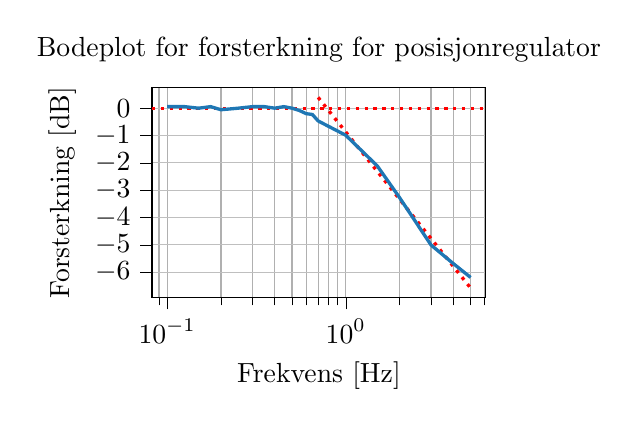
\begin{tikzpicture}

\definecolor{darkgray176}{RGB}{176,176,176}
\definecolor{orange}{RGB}{255,165,0}
\definecolor{steelblue31119180}{RGB}{31,119,180}

\begin{axis}[
grid=both,
tick align=outside,
tick pos=left,
title={Bodeplot for forsterkning for posisjonregulator},
x grid style={darkgray176},
height=\figH,
width=\figW,
xlabel={Frekvens [Hz]},
xmajorgrids,
xmin=0.0822340159426889, xmax=6.08020895329329,
xminorgrids,
xmode=log,
xtick style={color=black},
xtick={0.001,0.01,0.1,1,10,100},
xticklabels={
  \(\displaystyle {10^{-3}}\),
  \(\displaystyle {10^{-2}}\),
  \(\displaystyle {10^{-1}}\),
  \(\displaystyle {10^{0}}\),
  \(\displaystyle {10^{1}}\),
  \(\displaystyle {10^{2}}\)
},
ylabel={Forsterkning [dB]},
ymin=-6.92696915493292, ymax=0.742898747755512,
ytick style={color=black},
ytick={-7,-6,-5,-4,-3,-2,-1,0,1},
yticklabels={
  \(\displaystyle {\ensuremath{-}7}\),
  \(\displaystyle {\ensuremath{-}6}\),
  \(\displaystyle {\ensuremath{-}5}\),
  \(\displaystyle {\ensuremath{-}4}\),
  \(\displaystyle {\ensuremath{-}3}\),
  \(\displaystyle {\ensuremath{-}2}\),
  \(\displaystyle {\ensuremath{-}1}\),
  \(\displaystyle {0}\),
  \(\displaystyle {1}\)
}
]
\addplot [very thick, dotted, red]
table {%
0.0822340159426889 0
6.08020895329329 0
};
\addplot [very thick, dotted, red]
table {%
0.7 0.394268388542402
1.17777777777778 -1.45093493262608
1.65555555555556 -2.65850703298998
2.13333333333333 -3.55769144857336
2.61111111111111 -4.27438234056457
3.08888888888889 -4.87030247038411
3.56666666666667 -5.38034462173227
4.04444444444444 -5.8261713110089
4.52222222222222 -6.22215903826441
5 -6.57833879571981
};
\addplot [very thick, steelblue31119180]
table {%
0.1 0.0565858003772851
0.125 0.0565858003772851
0.15 0
0.175 0.0565858003772851
0.2 -0.0569568574565249
0.25 0
0.3 0.0565858003772851
0.35 0.0565858003772851
0.4 0
0.45 0.0565858003772851
0.5 0
0.55 -0.0855759595855004
0.6 -0.201004763143006
0.65 -0.230103248106495
0.7 -0.466468571652479
1 -0.99117558881648
1.5 -2.11020369539948
2 -3.27004263495321
3 -5.00385959148062
4 -5.68648604322257
5 -6.19260334851798
};
\end{axis}

\end{tikzpicture}

    \caption{Bodeplot for forstkerningen til systemet med posisjonsregulatoren. De røde stiplede linjene er pålagt grafikk, for å lettere finne knekkfrekvensen.}
    \label{fig:bodeplot}
\end{figure}

\begin{figure}[h!]
    \centering
    % This file was created with tikzplotlib v0.10.1.
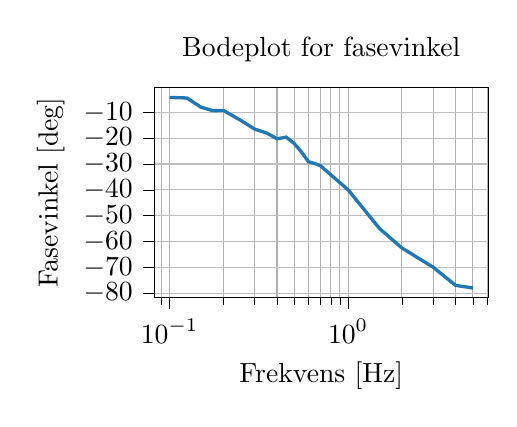
\begin{tikzpicture}

\definecolor{darkgray176}{RGB}{176,176,176}
\definecolor{steelblue31119180}{RGB}{31,119,180}

\begin{axis}[
grid=both,
tick align=outside,
tick pos=left,
title={Bodeplot for fasevinkel},
x grid style={darkgray176},
height=\figH,
width=\figW,
xlabel={Frekvens [Hz]},
xmajorgrids,
xmin=0.0822340159426889, xmax=6.08020895329329,
xminorgrids,
xmode=log,
xtick style={color=black},
xtick={0.001,0.01,0.1,1,10,100},
xticklabels={
  \(\displaystyle {10^{-3}}\),
  \(\displaystyle {10^{-2}}\),
  \(\displaystyle {10^{-1}}\),
  \(\displaystyle {10^{0}}\),
  \(\displaystyle {10^{1}}\),
  \(\displaystyle {10^{2}}\)
},
ylabel={Fasevinkel [deg]},
ymin=-81.689, ymax=-0.531,
ytick style={color=black},
ytick={-90,-80,-70,-60,-50,-40,-30,-20,-10,0},
yticklabels={
  \(\displaystyle {\ensuremath{-}90}\),
  \(\displaystyle {\ensuremath{-}80}\),
  \(\displaystyle {\ensuremath{-}70}\),
  \(\displaystyle {\ensuremath{-}60}\),
  \(\displaystyle {\ensuremath{-}50}\),
  \(\displaystyle {\ensuremath{-}40}\),
  \(\displaystyle {\ensuremath{-}30}\),
  \(\displaystyle {\ensuremath{-}20}\),
  \(\displaystyle {\ensuremath{-}10}\),
  \(\displaystyle {0}\)
}
]
\addplot [very thick, steelblue31119180]
table {%
0.1 -4.22
0.125 -4.44
0.15 -8
0.175 -9.37
0.2 -9.26
0.25 -13.09
0.3 -16.5
0.35 -18
0.4 -20.25
0.45 -19.6
0.5 -22.11
0.55 -25.5
0.6 -29.15
0.65 -29.8
0.7 -30.69
1 -40
1.5 -55
2 -62.5
3 -70
4 -77
5 -78
};
\end{axis}

\end{tikzpicture}

    \caption{Bodeplot for fasevinkelen til systemet med posisjonsregulatoren.}
    \label{fig:bodeplot_fase}
\end{figure}






\subsection{Diskusjon}

\autoref{fig:posisjon_P_regulator} viser at regulatoren når referanseverdien uten stasjonæravvik. Det er verdt å legge merke til pulsen i starten av transienten. 
Det kan være flere årsaker for at dette oppstår, deriblant induksjon fra pådragstrømmen til målestrømmen.

Det er også et lite oversving i posisjonsregulatoren, til tross for at posisjonsregulatoren er av første orden. Dette kan skje siden hele systemet er reulgert av en en kaskaderegulator av høyere orden.

Under tuning av reguleringen i hastighets- og posisjonsregulatoren var det vanskelig å finne et sett med parametere til potensiometerene for å få en god respons på posisjonsreguleringen. 
Ved de fleste kombinasjoner av parametere endte motoren opp med å vibrere med høy frekvens rundt referansepunktet. 
Dette kan ha blitt forårsaket av systemet er veldig sensitivt til støy eller at det har vært veldig mye støy i kretsen.
Reguleringen fungerte veldig bra ved bruk av kun proporsjonalvirkning som kommer av at det ikke er noen krefter som hindrer servomotoren i å holde en konstant posisjon.
Derfor ble reguleringen kanskje best ved et veldig lavt proporsjonal-ledd og lite til ingen integrasjonsvirkning.


Bode-plottet i \autoref{fig:bodeplot} har et knekkpunkt omtrent ved \SI{0.8}{\hertz}. Det vil si at motoren ikke klarer å følge referansen dersom den endrer seg fortere enn knekkfkrevensen. Det gjør at motoren ikke oscillerer over hele området til referansen, kun et mindre område. 

\autoref{fig:bodeplot_fase} viser et faseskifte ved høye frekvenser. Det vil si at motoren henger etter referansen, siden referansen endres så fort. Motoren henger etter ganske allerede fra \SI{0.1}{\hertz}, men er ikke spesielt merkbart før knekkfrekvensen.






















% Dersom dere ønsker å tegne kretsskjema med Tikz, finner dere et eksempel i filen
% \texttt{kretsskjema.tex} under \texttt{figurer}. Resultatet kan dere se i 
% Figur \ref{fig:kretsskjema}. Det er ikke nødvendig å bruke tikz for å tegne kretsskjema, dere kan også bruke andre (mer brukervennlige) programmer. Pass på at 
% det er lett å lese kretsskjemaet når dere har satt det inn i rapporten deres!

% \begin{figure}[t]
%     \centering
%     \def\x{4}
\def\y{4}
% Size of the bridge
\def\dx{1.5}
\def\dy{1.5}
\begin{circuitikz}[american voltages]
  \node at (\x+2*\dx,\y) {} ;
  % Voltage source
  \draw (0,0) to [V, l_=$V$,invert]
  (0, \y) to (\x, \y)
  % Left half bridge
  to [R, l_=$R_1$, -] (\x-\dx,\y-\dy) % Top left resistor
  to [R, l_=$R_2$, -] (\x,\y-2*\dy);  % Bottom left resistor
  % Right half bridge
  \draw (\x,\y)
  to [R, l_=$R_3$, -] (\x+\dx, \y-\dy) % Top right resistor
  to [R, l_=$R_T$, -] (\x,\y-2*\dy)  % Bottom left resistor
  % Draw connection to (-) terminal of voltage source
  to (\x, 0) to (0,0);

  % Draw amplifer
  \draw (\x-\dx, \y-\dy) to (\x-1.2*\dx, \y-\dy)
  %\draw (\x-1.5\dx, \y-\dy) 
  to (\x-1.2*\dx, \y-1)
  to[crossing] (\x-1.2*\dx, \y+1) to [short,-*](\x+2*\dx,\y+1);
  \draw (\x+\dx, \y-\dy) to (\x+1.2*\dx, \y-\dy)
  to (\x+1.2*\dx, \y-1)
  to [short,-*](\x+2*\dx,\y-1);
\end{circuitikz}
%     \caption{Eksempel på kretsskjema fra Eksamen i TTK4101 2021.}
%     \label{fig:kretsskjema}
% \end{figure}

% Dersom dere eksporterer plots som eps, bruker vi kommandoen \texttt{includegraphics}
% for å tegne figuren, som vist i kildekoden. Resultatet er vist i Figur 
% \ref{fig:eps_eksempel}.

% \begin{figure}[t]
% \centering
% 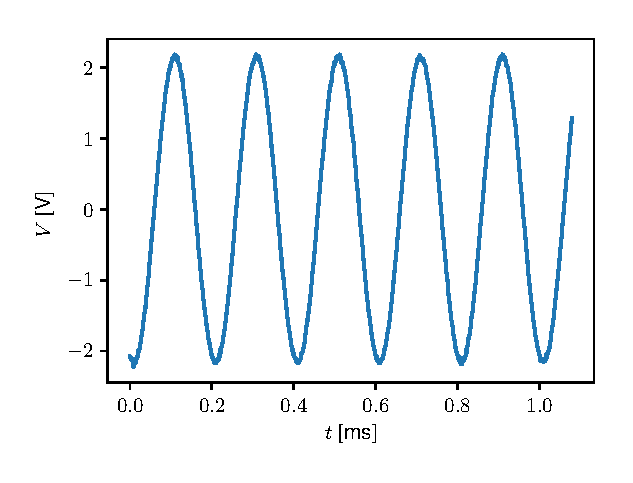
\includegraphics[width=0.4\textwidth]{figurer/eksempel_plott.eps}
% \caption{Eksempel på plott med eps-fil. Merk at fontstørrelsen er mindre enn i
% resten av dokumentet, ettersom den er styrt av figurstørrelsen når vi laget plottet.}
% \label{fig:eps_eksempel}
% \end{figure}

% Dersom dere eksporterer figurene deres som tikz, bruker vi kommandoen \texttt{\\input}
% for å vise figuren. Resultatet er vist i Figur \ref{fig:tikz_eksempel}.
% \setlength{\figW}{0.4\textwidth}
% \setlength{\figH}{0.35\textwidth}
% \begin{figure}[t]
%     \centering
%     % This file was created by tikzplotlib v0.9.8.
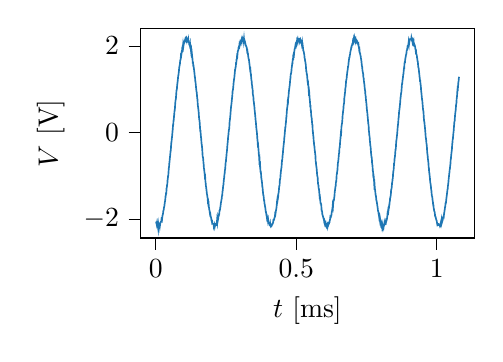
\begin{tikzpicture}

\definecolor{color0}{rgb}{0.12156862745098,0.466666666666667,0.705882352941177}

\begin{axis}[
height=\figH,
tick align=outside,
tick pos=left,
width=\figW,
x grid style={white!69.0196078431373!black},
xlabel={\(\displaystyle t\) [ms]},
xmin=-0.053988, xmax=1.133748,
xtick style={color=black},
y grid style={white!69.0196078431373!black},
ylabel={\(\displaystyle V\) [V]},
ymin=-2.441895, ymax=2.402835,
ytick style={color=black}
]
\addplot [semithick, color0]
table {%
0 -2.0752
0.000880000000000195 -2.0752
0.00176000000000017 -2.08496
0.00264000000000015 -2.09473
0.00352000000000013 -2.12402
0.00440000000000011 -2.09473
0.00528000000000008 -2.13379
0.00616000000000006 -2.11426
0.00704000000000004 -2.13379
0.00792000000000002 -2.18262
0.0088 -2.22168
0.00968000000000019 -2.13379
0.0105600000000002 -2.17285
0.0114400000000001 -2.14355
0.0123200000000001 -2.11426
0.0132000000000001 -2.10449
0.0140800000000001 -2.10449
0.0149600000000001 -2.16309
0.01584 -2.12402
0.01672 -2.08496
0.0176 -2.0752
0.0184800000000002 -2.06543
0.0193600000000002 -2.06543
0.0202400000000001 -2.06543
0.0211200000000001 -1.97754
0.0220000000000001 -1.97754
0.0228800000000001 -1.99707
0.0237600000000001 -1.94824
0.02464 -1.90918
0.02552 -1.89941
0.0264 -1.86035
0.0272800000000002 -1.81152
0.0281600000000002 -1.80176
0.0290400000000001 -1.7627
0.0299200000000001 -1.72363
0.0308000000000001 -1.7041
0.0316800000000001 -1.65527
0.0325600000000001 -1.61621
0.03344 -1.58691
0.03432 -1.53809
0.0352 -1.46973
0.0360800000000002 -1.45996
0.0369600000000002 -1.40137
0.0378400000000001 -1.40137
0.0387200000000001 -1.29395
0.0396000000000001 -1.27441
0.0404800000000001 -1.21582
0.04136 -1.19629
0.04224 -1.1084
0.04312 -1.06934
0.0440000000000002 -1.01074
0.0448800000000002 -0.991211
0.0457600000000002 -0.913086
0.0466400000000001 -0.825195
0.0475200000000001 -0.795898
0.0484000000000001 -0.717773
0.0492800000000001 -0.678711
0.0501600000000001 -0.610352
0.05104 -0.561523
0.05192 -0.50293
0.0528000000000002 -0.43457
0.0536800000000002 -0.424805
0.0545600000000002 -0.327148
0.0554400000000001 -0.249023
0.0563200000000001 -0.219727
0.0572000000000001 -0.151367
0.0580800000000001 -0.112305
0.05896 -0.0537109
0.05984 0.0244141
0.06072 0.0634766
0.0616000000000002 0.170898
0.0624800000000002 0.180664
0.0633600000000002 0.268555
0.0642400000000001 0.288086
0.0651200000000001 0.366211
0.0660000000000001 0.415039
0.0668800000000001 0.493164
0.06776 0.512695
0.06864 0.571289
0.06952 0.668945
0.0704000000000002 0.727539
0.0712800000000002 0.756836
0.0721600000000002 0.795898
0.0730400000000001 0.883789
0.0739200000000001 0.961914
0.0748000000000001 0.981445
0.0756800000000001 1.02051
0.07656 1.09863
0.07744 1.1377
0.07832 1.18652
0.0792000000000002 1.24512
0.0800800000000002 1.30371
0.0809600000000001 1.32324
0.0818400000000001 1.37207
0.0827200000000001 1.4209
0.0836000000000001 1.48926
0.0844800000000001 1.52832
0.08536 1.54785
0.08624 1.58691
0.08712 1.65527
0.0880000000000002 1.6748
0.0888800000000002 1.69434
0.0897600000000001 1.77246
0.0906400000000001 1.7627
0.0915200000000001 1.80176
0.0924000000000001 1.86035
0.0932800000000001 1.86035
0.09416 1.91895
0.09504 1.90918
0.09592 1.96777
0.0968000000000002 1.95801
0.0976800000000002 2.02637
0.0985600000000001 1.9873
0.0994400000000001 2.02637
0.10032 2.0459
0.1012 2.0752
0.10208 2.09473
0.10296 2.11426
0.10384 2.12402
0.10472 2.14355
0.1056 2.11426
0.10648 2.12402
0.10736 2.14355
0.10824 2.17285
0.10912 2.18262
0.11 2.14355
0.11088 2.17285
0.11176 2.17285
0.11264 2.14355
0.11352 2.12402
0.1144 2.10449
0.11528 2.11426
0.11616 2.14355
0.11704 2.09473
0.11792 2.0752
0.1188 2.06543
0.11968 2.02637
0.12056 2.02637
0.12144 2.00684
0.12232 2.03613
0.1232 1.94824
0.12408 1.93848
0.12496 1.91895
0.12584 1.87012
0.12672 1.89941
0.1276 1.82129
0.12848 1.84082
0.12936 1.78223
0.13024 1.7334
0.13112 1.68457
0.132 1.60645
0.13288 1.60645
0.13376 1.53809
0.13464 1.53809
0.13552 1.48926
0.1364 1.45996
0.13728 1.40137
0.13816 1.3623
0.13904 1.28418
0.13992 1.27441
0.1408 1.18652
0.14168 1.16699
0.14256 1.1084
0.14344 1.0498
0.14432 0.991211
0.1452 0.942383
0.14608 0.922852
0.14696 0.854492
0.14784 0.786133
0.14872 0.756836
0.1496 0.649414
0.15048 0.600586
0.15136 0.561523
0.15224 0.512695
0.15312 0.454102
0.154 0.366211
0.15488 0.297852
0.15576 0.27832
0.15664 0.219727
0.15752 0.131836
0.1584 0.0439453
0.15928 0.0439453
0.16016 -0.0341797
0.16104 -0.102539
0.16192 -0.141602
0.1628 -0.229492
0.16368 -0.27832
0.16456 -0.317383
0.16544 -0.375977
0.16632 -0.463867
0.1672 -0.561523
0.16808 -0.571289
0.16896 -0.610352
0.16984 -0.688477
0.17072 -0.737305
0.1716 -0.825195
0.17248 -0.854492
0.17336 -0.913086
0.17424 -0.961914
0.17512 -1.03027
0.176 -1.02051
0.17688 -1.12793
0.17776 -1.16699
0.17864 -1.23535
0.17952 -1.26465
0.1804 -1.31348
0.18128 -1.3623
0.18216 -1.4209
0.18304 -1.44043
0.18392 -1.48926
0.1848 -1.51855
0.18568 -1.59668
0.18656 -1.58691
0.18744 -1.65527
0.18832 -1.64551
0.1892 -1.72363
0.19008 -1.75293
0.19096 -1.79199
0.19184 -1.82129
0.19272 -1.86035
0.1936 -1.89941
0.19448 -1.88965
0.19536 -1.93848
0.19624 -1.95801
0.19712 -1.96777
0.198 -2.00684
0.19888 -2.0459
0.19976 -2.0459
0.20064 -2.08496
0.20152 -2.0752
0.2024 -2.11426
0.20328 -2.11426
0.20416 -2.11426
0.20504 -2.11426
0.20592 -2.12402
0.2068 -2.17285
0.20768 -2.15332
0.20856 -2.15332
0.20944 -2.13379
0.21032 -2.17285
0.2112 -2.14355
0.21208 -2.15332
0.21296 -2.14355
0.21384 -2.14355
0.21472 -2.11426
0.2156 -2.11426
0.21648 -2.12402
0.21736 -2.11426
0.21824 -2.0459
0.21912 -2.08496
0.22 -2.02637
0.22088 -1.97754
0.22176 -2.0166
0.22264 -1.9873
0.22352 -1.93848
0.2244 -1.92871
0.22528 -1.90918
0.22616 -1.88965
0.22704 -1.81152
0.22792 -1.81152
0.2288 -1.78223
0.22968 -1.74316
0.23056 -1.71387
0.23144 -1.66504
0.23232 -1.61621
0.2332 -1.59668
0.23408 -1.55762
0.23496 -1.52832
0.23584 -1.46973
0.23672 -1.45996
0.2376 -1.38184
0.23848 -1.34277
0.23936 -1.29395
0.24024 -1.23535
0.24112 -1.20605
0.242 -1.1377
0.24288 -1.0791
0.24376 -1.04004
0.24464 -0.97168
0.24552 -0.942383
0.2464 -0.874023
0.24728 -0.844727
0.24816 -0.766602
0.24904 -0.688477
0.24992 -0.678711
0.2508 -0.600586
0.25168 -0.551758
0.25256 -0.483398
0.25344 -0.43457
0.25432 -0.375977
0.2552 -0.297852
0.25608 -0.239258
0.25696 -0.180664
0.25784 -0.102539
0.25872 -0.0634766
0.2596 0.00488281
0.26048 0.0537109
0.26136 0.0732422
0.26224 0.141602
0.26312 0.249023
0.264 0.288086
0.26488 0.336914
0.26576 0.395508
0.26664 0.473633
0.26752 0.541992
0.2684 0.600586
0.26928 0.639648
0.27016 0.688477
0.27104 0.74707
0.27192 0.805664
0.2728 0.864258
0.27368 0.952148
0.27456 0.97168
0.27544 1.01074
0.27632 1.06934
0.2772 1.1377
0.27808 1.18652
0.27896 1.23535
0.27984 1.26465
0.28072 1.32324
0.2816 1.38184
0.28248 1.4502
0.28336 1.45996
0.28424 1.50879
0.28512 1.51855
0.286 1.60645
0.28688 1.60645
0.28776 1.68457
0.28864 1.69434
0.28952 1.7627
0.2904 1.75293
0.29128 1.82129
0.29216 1.87012
0.29304 1.88965
0.29392 1.89941
0.2948 1.95801
0.29568 1.96777
0.29656 1.9873
0.29744 1.97754
0.29832 2.0459
0.2992 2.03613
0.30008 2.06543
0.30096 2.0459
0.30184 2.06543
0.30272 2.11426
0.3036 2.11426
0.30448 2.13379
0.30536 2.14355
0.30624 2.16309
0.30712 2.11426
0.308 2.14355
0.30888 2.18262
0.30976 2.17285
0.31064 2.16309
0.31152 2.16309
0.3124 2.16309
0.31328 2.11426
0.31416 2.16309
0.31504 2.10449
0.31592 2.09473
0.3168 2.11426
0.31768 2.09473
0.31856 2.06543
0.31944 2.0459
0.32032 2.0166
0.3212 2.00684
0.32208 1.9873
0.32296 1.97754
0.32384 1.95801
0.32472 1.91895
0.3256 1.87012
0.32648 1.87988
0.32736 1.84082
0.32824 1.82129
0.32912 1.7627
0.33 1.72363
0.33088 1.69434
0.33176 1.68457
0.33264 1.63574
0.33352 1.58691
0.3344 1.53809
0.33528 1.48926
0.33616 1.44043
0.33704 1.4502
0.33792 1.35254
0.3388 1.35254
0.33968 1.27441
0.34056 1.21582
0.34144 1.18652
0.34232 1.1084
0.3432 1.0791
0.34408 1.01074
0.34496 1.00098
0.34584 0.874023
0.34672 0.854492
0.3476 0.825195
0.34848 0.727539
0.34936 0.698242
0.35024 0.639648
0.35112 0.600586
0.352 0.522461
0.35288 0.473633
0.35376 0.415039
0.35464 0.356445
0.35552 0.288086
0.3564 0.239258
0.35728 0.170898
0.35816 0.102539
0.35904 0.0537109
0.35992 0.0146484
0.3608 -0.0537109
0.36168 -0.141602
0.36256 -0.200195
0.36344 -0.288086
0.36432 -0.27832
0.3652 -0.34668
0.36608 -0.415039
0.36696 -0.50293
0.36784 -0.541992
0.36872 -0.639648
0.3696 -0.620117
0.37048 -0.737305
0.37136 -0.727539
0.37224 -0.844727
0.37312 -0.913086
0.374 -0.913086
0.37488 -0.952148
0.37576 -1.0498
0.37664 -1.0791
0.37752 -1.12793
0.3784 -1.15723
0.37928 -1.24512
0.38016 -1.26465
0.38104 -1.33301
0.38192 -1.3916
0.3828 -1.4502
0.38368 -1.45996
0.38456 -1.50879
0.38544 -1.56738
0.38632 -1.57715
0.3872 -1.64551
0.38808 -1.66504
0.38896 -1.7041
0.38984 -1.7334
0.39072 -1.77246
0.3916 -1.83105
0.39248 -1.84082
0.39336 -1.87988
0.39424 -1.90918
0.39512 -1.94824
0.396 -1.9873
0.39688 -1.96777
0.39776 -1.99707
0.39864 -2.0166
0.39952 -2.05566
0.4004 -2.02637
0.40128 -2.0752
0.40216 -2.08496
0.40304 -2.09473
0.40392 -2.10449
0.4048 -2.10449
0.40568 -2.14355
0.40656 -2.14355
0.40744 -2.11426
0.40832 -2.16309
0.4092 -2.17285
0.41008 -2.15332
0.41096 -2.17285
0.41184 -2.17285
0.41272 -2.14355
0.4136 -2.14355
0.41448 -2.13379
0.41536 -2.12402
0.41624 -2.11426
0.41712 -2.09473
0.418 -2.08496
0.41888 -2.02637
0.41976 -2.02637
0.42064 -2.02637
0.42152 -2.0166
0.4224 -1.97754
0.42328 -1.96777
0.42416 -1.94824
0.42504 -1.88965
0.42592 -1.89941
0.4268 -1.86035
0.42768 -1.82129
0.42856 -1.79199
0.42944 -1.7627
0.43032 -1.71387
0.4312 -1.64551
0.43208 -1.58691
0.43296 -1.54785
0.43384 -1.56738
0.43472 -1.52832
0.4356 -1.50879
0.43648 -1.4209
0.43736 -1.40137
0.43824 -1.35254
0.43912 -1.28418
0.44 -1.23535
0.44088 -1.22559
0.44176 -1.11816
0.44264 -1.0791
0.44352 -1.05957
0.4444 -0.981445
0.44528 -0.922852
0.44616 -0.874023
0.44704 -0.834961
0.44792 -0.795898
0.4488 -0.708008
0.44968 -0.649414
0.45056 -0.629883
0.45144 -0.541992
0.45232 -0.512695
0.4532 -0.43457
0.45408 -0.366211
0.45496 -0.317383
0.45584 -0.258789
0.45672 -0.219727
0.4576 -0.131836
0.45848 -0.0927734
0.45936 -0.0146484
0.46024 0.0439453
0.46112 0.112305
0.462 0.12207
0.46288 0.209961
0.46376 0.239258
0.46464 0.336914
0.46552 0.366211
0.4664 0.463867
0.46728 0.532227
0.46816 0.571289
0.46904 0.610352
0.46992 0.708008
0.4708 0.698242
0.47168 0.805664
0.47256 0.81543
0.47344 0.90332
0.47432 0.961914
0.4752 1.00098
0.47608 1.0498
0.47696 1.08887
0.47784 1.14746
0.47872 1.22559
0.4796 1.25488
0.48048 1.34277
0.48136 1.35254
0.48224 1.38184
0.48312 1.4209
0.484 1.48926
0.48488 1.52832
0.48576 1.58691
0.48664 1.58691
0.48752 1.6748
0.4884 1.6748
0.48928 1.74316
0.49016 1.7334
0.49104 1.79199
0.49192 1.78223
0.4928 1.84082
0.49368 1.88965
0.49456 1.92871
0.49544 1.93848
0.49632 1.96777
0.4972 2.00684
0.49808 2.0459
0.49896 2.06543
0.49984 2.0752
0.50072 2.0459
0.5016 2.08496
0.50248 2.08496
0.50336 2.14355
0.50424 2.13379
0.50512 2.15332
0.506 2.11426
0.50688 2.15332
0.50776 2.14355
0.50864 2.15332
0.50952 2.15332
0.5104 2.13379
0.51128 2.11426
0.51216 2.18262
0.51304 2.13379
0.51392 2.14355
0.5148 2.0752
0.51568 2.14355
0.51656 2.0752
0.51744 2.06543
0.51832 2.05566
0.5192 2.0752
0.52008 2.03613
0.52096 2.06543
0.52184 1.96777
0.52272 1.96777
0.5236 1.9873
0.52448 1.93848
0.52536 1.88965
0.52624 1.87988
0.52712 1.86035
0.528 1.82129
0.52888 1.79199
0.52976 1.72363
0.53064 1.7041
0.53152 1.66504
0.5324 1.63574
0.53328 1.59668
0.53416 1.56738
0.53504 1.47949
0.53592 1.41113
0.5368 1.40137
0.53768 1.34277
0.53856 1.33301
0.53944 1.26465
0.54032 1.18652
0.5412 1.14746
0.54208 1.15723
0.54296 1.08887
0.54384 1.04004
0.54472 0.952148
0.5456 0.97168
0.54648 0.922852
0.54736 0.825195
0.54824 0.756836
0.54912 0.708008
0.55 0.610352
0.55088 0.610352
0.55176 0.50293
0.55264 0.493164
0.55352 0.385742
0.5544 0.356445
0.55528 0.317383
0.55616 0.249023
0.55704 0.180664
0.55792 0.170898
0.5588 0.0341797
0.55968 0.00488281
0.56056 -0.0732422
0.56144 -0.102539
0.56232 -0.200195
0.5632 -0.239258
0.56408 -0.307617
0.56496 -0.327148
0.56584 -0.405273
0.56672 -0.444336
0.5676 -0.493164
0.56848 -0.541992
0.56936 -0.668945
0.57024 -0.698242
0.57112 -0.766602
0.572 -0.795898
0.57288 -0.844727
0.57376 -0.913086
0.57464 -0.991211
0.57552 -1.02051
0.5764 -1.04004
0.57728 -1.14746
0.57816 -1.20605
0.57904 -1.21582
0.57992 -1.29395
0.5808 -1.30371
0.58168 -1.35254
0.58256 -1.4209
0.58344 -1.48926
0.58432 -1.47949
0.5852 -1.52832
0.58608 -1.60645
0.58696 -1.64551
0.58784 -1.64551
0.58872 -1.65527
0.5896 -1.71387
0.59048 -1.81152
0.59136 -1.81152
0.59224 -1.83105
0.59312 -1.89941
0.594 -1.90918
0.59488 -1.92871
0.59576 -1.95801
0.59664 -1.96777
0.59752 -1.99707
0.5984 -2.0166
0.59928 -2.03613
0.60016 -2.08496
0.60104 -2.10449
0.60192 -2.06543
0.6028 -2.08496
0.60368 -2.11426
0.60456 -2.13379
0.60544 -2.11426
0.60632 -2.14355
0.6072 -2.15332
0.60808 -2.17285
0.60896 -2.15332
0.60984 -2.16309
0.61072 -2.14355
0.6116 -2.17285
0.61248 -2.13379
0.61336 -2.14355
0.61424 -2.11426
0.61512 -2.12402
0.616 -2.10449
0.61688 -2.10449
0.61776 -2.0752
0.61864 -2.0752
0.61952 -2.03613
0.6204 -2.0166
0.62128 -1.96777
0.62216 -1.97754
0.62304 -1.96777
0.62392 -1.92871
0.6248 -1.92871
0.62568 -1.89941
0.62656 -1.84082
0.62744 -1.82129
0.62832 -1.78223
0.6292 -1.75293
0.63008 -1.68457
0.63096 -1.71387
0.63184 -1.63574
0.63272 -1.58691
0.6336 -1.57715
0.63448 -1.55762
0.63536 -1.50879
0.63624 -1.46973
0.63712 -1.38184
0.638 -1.34277
0.63888 -1.30371
0.63976 -1.25488
0.64064 -1.23535
0.64152 -1.14746
0.6424 -1.1377
0.64328 -1.06934
0.64416 -0.97168
0.64504 -0.952148
0.64592 -0.90332
0.6468 -0.874023
0.64768 -0.776367
0.64856 -0.708008
0.64944 -0.678711
0.65032 -0.629883
0.6512 -0.561523
0.65208 -0.50293
0.65296 -0.473633
0.65384 -0.366211
0.65472 -0.356445
0.6556 -0.288086
0.65648 -0.209961
0.65736 -0.151367
0.65824 -0.0830078
0.65912 -0.0146484
0.66 -0.0244141
0.66088 0.112305
0.66176 0.161133
0.66264 0.19043
0.66352 0.229492
0.6644 0.297852
0.66528 0.395508
0.66616 0.43457
0.66704 0.493164
0.66792 0.532227
0.6688 0.620117
0.66968 0.649414
0.67056 0.688477
0.67144 0.805664
0.67232 0.834961
0.6732 0.893555
0.67408 0.932617
0.67496 1.02051
0.67584 1.04004
0.67672 1.1084
0.6776 1.18652
0.67848 1.21582
0.67936 1.23535
0.68024 1.30371
0.68112 1.35254
0.682 1.40137
0.68288 1.43066
0.68376 1.47949
0.68464 1.52832
0.68552 1.53809
0.6864 1.60645
0.68728 1.65527
0.68816 1.69434
0.68904 1.7334
0.68992 1.7334
0.6908 1.78223
0.69168 1.80176
0.69256 1.85059
0.69344 1.87988
0.69432 1.89941
0.6952 1.92871
0.69608 1.96777
0.69696 1.96777
0.69784 2.00684
0.69872 2.0166
0.6996 2.0459
0.70048 2.05566
0.70136 2.06543
0.70224 2.12402
0.70312 2.11426
0.704 2.09473
0.70488 2.14355
0.70576 2.11426
0.70664 2.12402
0.70752 2.17285
0.7084 2.14355
0.70928 2.12402
0.71016 2.14355
0.71104 2.11426
0.71192 2.13379
0.7128 2.09473
0.71368 2.11426
0.71456 2.11426
0.71544 2.12402
0.71632 2.11426
0.7172 2.10449
0.71808 2.0752
0.71896 2.05566
0.71984 2.0459
0.72072 2.02637
0.7216 2.03613
0.72248 1.97754
0.72336 1.96777
0.72424 1.90918
0.72512 1.91895
0.726 1.85059
0.72688 1.83105
0.72776 1.82129
0.72864 1.77246
0.72952 1.7627
0.7304 1.71387
0.73128 1.68457
0.73216 1.64551
0.73304 1.58691
0.73392 1.52832
0.7348 1.51855
0.73568 1.44043
0.73656 1.40137
0.73744 1.38184
0.73832 1.35254
0.7392 1.26465
0.74008 1.25488
0.74096 1.18652
0.74184 1.14746
0.74272 1.1084
0.7436 1.04004
0.74448 0.991211
0.74536 0.961914
0.74624 0.874023
0.74712 0.844727
0.748 0.776367
0.74888 0.717773
0.74976 0.678711
0.75064 0.610352
0.75152 0.532227
0.7524 0.483398
0.75328 0.444336
0.75416 0.375977
0.75504 0.317383
0.75592 0.249023
0.7568 0.19043
0.75768 0.161133
0.75856 0.0537109
0.75944 -0.00488281
0.76032 -0.0732422
0.7612 -0.0927734
0.76208 -0.180664
0.76296 -0.239258
0.76384 -0.307617
0.76472 -0.327148
0.7656 -0.405273
0.76648 -0.483398
0.76736 -0.532227
0.76824 -0.581055
0.76912 -0.59082
0.77 -0.698242
0.77088 -0.737305
0.77176 -0.786133
0.77264 -0.883789
0.77352 -0.90332
0.7744 -1.00098
0.77528 -0.991211
0.77616 -1.03027
0.77704 -1.11816
0.77792 -1.21582
0.7788 -1.19629
0.77968 -1.28418
0.78056 -1.32324
0.78144 -1.3623
0.78232 -1.43066
0.7832 -1.45996
0.78408 -1.47949
0.78496 -1.55762
0.78584 -1.57715
0.78672 -1.60645
0.7876 -1.63574
0.78848 -1.68457
0.78936 -1.71387
0.79024 -1.7627
0.79112 -1.81152
0.792 -1.82129
0.79288 -1.86035
0.79376 -1.89941
0.79464 -1.91895
0.79552 -1.96777
0.7964 -1.94824
0.79728 -2.00684
0.79816 -2.0459
0.79904 -2.0166
0.79992 -2.05566
0.8008 -2.09473
0.80168 -2.06543
0.80256 -2.0752
0.80344 -2.12402
0.80432 -2.10449
0.8052 -2.15332
0.80608 -2.11426
0.80696 -2.14355
0.80784 -2.18262
0.80872 -2.14355
0.8096 -2.15332
0.81048 -2.15332
0.81136 -2.18262
0.81224 -2.14355
0.81312 -2.14355
0.814 -2.09473
0.81488 -2.12402
0.81576 -2.12402
0.81664 -2.12402
0.81752 -2.10449
0.8184 -2.0752
0.81928 -2.08496
0.82016 -2.0459
0.82104 -1.97754
0.82192 -2.02637
0.8228 -2.00684
0.82368 -1.96777
0.82456 -1.91895
0.82544 -1.84082
0.82632 -1.84082
0.8272 -1.80176
0.82808 -1.82129
0.82896 -1.77246
0.82984 -1.7627
0.83072 -1.68457
0.8316 -1.68457
0.83248 -1.61621
0.83336 -1.59668
0.83424 -1.51855
0.83512 -1.50879
0.836 -1.46973
0.83688 -1.43066
0.83776 -1.34277
0.83864 -1.31348
0.83952 -1.29395
0.8404 -1.23535
0.84128 -1.16699
0.84216 -1.1377
0.84304 -1.0791
0.84392 -1.05957
0.8448 -0.961914
0.84568 -0.90332
0.84656 -0.874023
0.84744 -0.81543
0.84832 -0.717773
0.8492 -0.708008
0.85008 -0.610352
0.85096 -0.581055
0.85184 -0.532227
0.85272 -0.454102
0.8536 -0.395508
0.85448 -0.385742
0.85536 -0.27832
0.85624 -0.200195
0.85712 -0.170898
0.858 -0.112305
0.85888 -0.0634766
0.85976 -0.00488281
0.86064 0.0732422
0.86152 0.141602
0.8624 0.180664
0.86328 0.239258
0.86416 0.327148
0.86504 0.356445
0.86592 0.454102
0.8668 0.50293
0.86768 0.541992
0.86856 0.59082
0.86944 0.649414
0.87032 0.708008
0.8712 0.795898
0.87208 0.825195
0.87296 0.893555
0.87384 0.913086
0.87472 0.961914
0.8756 1.04004
0.87648 1.11816
0.87736 1.12793
0.87824 1.19629
0.87912 1.22559
0.88 1.27441
0.88088 1.33301
0.88176 1.35254
0.88264 1.4209
0.88352 1.47949
0.8844 1.47949
0.88528 1.58691
0.88616 1.61621
0.88704 1.61621
0.88792 1.68457
0.8888 1.71387
0.88968 1.74316
0.89056 1.78223
0.89144 1.80176
0.89232 1.83105
0.8932 1.88965
0.89408 1.89941
0.89496 1.91895
0.89584 1.95801
0.89672 1.99707
0.8976 1.99707
0.89848 2.00684
0.89936 2.03613
0.90024 2.08496
0.90112 2.0459
0.902 2.11426
0.90288 2.09473
0.90376 2.13379
0.90464 2.14355
0.90552 2.14355
0.9064 2.15332
0.90728 2.15332
0.90816 2.14355
0.90904 2.14355
0.90992 2.18262
0.9108 2.15332
0.91168 2.16309
0.91256 2.15332
0.91344 2.11426
0.91432 2.15332
0.9152 2.14355
0.91608 2.12402
0.91696 2.08496
0.91784 2.10449
0.91872 2.03613
0.9196 2.0166
0.92048 2.02637
0.92136 2.00684
0.92224 2.00684
0.92312 1.97754
0.924 1.93848
0.92488 1.90918
0.92576 1.86035
0.92664 1.87012
0.92752 1.81152
0.9284 1.79199
0.92928 1.78223
0.93016 1.72363
0.93104 1.69434
0.93192 1.64551
0.9328 1.63574
0.93368 1.56738
0.93456 1.50879
0.93544 1.48926
0.93632 1.45996
0.9372 1.3916
0.93808 1.35254
0.93896 1.28418
0.93984 1.25488
0.94072 1.18652
0.9416 1.18652
0.94248 1.1084
0.94336 1.08887
0.94424 1.00098
0.94512 0.932617
0.946 0.893555
0.94688 0.825195
0.94776 0.766602
0.94864 0.737305
0.94952 0.678711
0.9504 0.600586
0.95128 0.541992
0.95216 0.50293
0.95304 0.473633
0.95392 0.366211
0.9548 0.288086
0.95568 0.249023
0.95656 0.219727
0.95744 0.151367
0.95832 0.102539
0.9592 0.0341797
0.96008 -0.0341797
0.96096 -0.112305
0.96184 -0.141602
0.96272 -0.19043
0.9636 -0.258789
0.96448 -0.288086
0.96536 -0.356445
0.96624 -0.463867
0.96712 -0.50293
0.968 -0.551758
0.96888 -0.620117
0.96976 -0.65918
0.97064 -0.708008
0.97152 -0.805664
0.9724 -0.834961
0.97328 -0.922852
0.97416 -0.952148
0.97504 -1.01074
0.97592 -1.05957
0.9768 -1.1377
0.97768 -1.17676
0.97856 -1.20605
0.97944 -1.25488
0.98032 -1.32324
0.9812 -1.34277
0.98208 -1.4209
0.98296 -1.46973
0.98384 -1.47949
0.98472 -1.51855
0.9856 -1.57715
0.98648 -1.60645
0.98736 -1.6748
0.98824 -1.6748
0.98912 -1.74316
0.99 -1.7627
0.99088 -1.81152
0.99176 -1.82129
0.99264 -1.84082
0.99352 -1.87988
0.9944 -1.93848
0.99528 -1.93848
0.99616 -1.94824
0.99704 -1.9873
0.99792 -2.00684
0.9988 -2.02637
0.99968 -2.03613
1.00056 -2.06543
1.00144 -2.10449
1.00232 -2.13379
1.0032 -2.12402
1.00408 -2.11426
1.00496 -2.11426
1.00584 -2.13379
1.00672 -2.14355
1.0076 -2.14355
1.00848 -2.13379
1.00936 -2.13379
1.01024 -2.13379
1.01112 -2.15332
1.012 -2.13379
1.01288 -2.14355
1.01376 -2.12402
1.01464 -2.09473
1.01552 -2.12402
1.0164 -2.09473
1.01728 -2.0459
1.01816 -2.09473
1.01904 -2.0752
1.01992 -2.02637
1.0208 -2.03613
1.02168 -2.0166
1.02256 -1.96777
1.02344 -1.94824
1.02432 -1.93848
1.0252 -1.94824
1.02608 -1.88965
1.02696 -1.86035
1.02784 -1.81152
1.02872 -1.78223
1.0296 -1.7334
1.03048 -1.71387
1.03136 -1.64551
1.03224 -1.64551
1.03312 -1.61621
1.034 -1.55762
1.03488 -1.50879
1.03576 -1.46973
1.03664 -1.4209
1.03752 -1.37207
1.0384 -1.32324
1.03928 -1.30371
1.04016 -1.22559
1.04104 -1.19629
1.04192 -1.1377
1.0428 -1.06934
1.04368 -1.02051
1.04456 -0.961914
1.04544 -0.922852
1.04632 -0.854492
1.0472 -0.834961
1.04808 -0.766602
1.04896 -0.727539
1.04984 -0.629883
1.05072 -0.600586
1.0516 -0.532227
1.05248 -0.483398
1.05336 -0.43457
1.05424 -0.385742
1.05512 -0.288086
1.056 -0.239258
1.05688 -0.170898
1.05776 -0.141602
1.05864 -0.0732422
1.05952 -0.0146484
1.0604 0.0341797
1.06128 0.112305
1.06216 0.180664
1.06304 0.249023
1.06392 0.258789
1.0648 0.34668
1.06568 0.415039
1.06656 0.463867
1.06744 0.50293
1.06832 0.571289
1.0692 0.649414
1.07008 0.65918
1.07096 0.766602
1.07184 0.805664
1.07272 0.864258
1.0736 0.961914
1.07448 1.02051
1.07536 1.01074
1.07624 1.0791
1.07712 1.15723
1.078 1.18652
1.07888 1.25488
1.07976 1.28418
};
\end{axis}

\end{tikzpicture}

%     \caption{Eksempel på plott med tikz-kode. Merk at fontstørrelsen er lik resten av dokumentet, ettersom den er styrt av Latex-kompilatoren.}
%     \label{fig:tikz_eksempel}
% \end{figure}


\section{Konklusjon}\label{sec:konklusjon}

Etter implementasjonen av fire forskjellige delsystemer; en hastighetsmåler, hastighetsregulator, posisjonsmåler og posisjonsregulator, og disse ble koblet sammen, endte man opp med en fullstendig og fungerende servomotor. 
Motoren har en rask respons opp til knekkfrekvensen på {\SI{0.8}{\hertz}}.

% \input simply inserts the contents of the file, while \include forces a \newpage.
% See \input vs. \include: http://tex.stackexchange.com/questions/246/when-should-i-use-input-vs-include

% References
%\newpage
\addcontentsline{toc}{section}{Kilder}
\printbibliography{}
\label{sec:bibliography}

\end{document}
